\RequirePackage[l2tabu,orthodox]{nag} % Раскомментировав, можно в логе получать рекомендации относительно правильного использования пакетов и предупреждения об устаревших и нерекомендуемых пакетах
% Формат А4, 14pt (ГОСТ Р 7.0.11-2011, 5.3.6)
\documentclass[a4paper,14pt]{extreport}
%\usepackage{csquotes}
%%% Проверка используемого TeX-движка %%%
\usepackage{iftex}
\newif\ifxetexorluatex   % определяем новый условный оператор (http://tex.stackexchange.com/a/47579/79756)
\ifXeTeX
    \xetexorluatextrue
\else
    \ifLuaTeX
        \xetexorluatextrue
    \else
        \xetexorluatexfalse
    \fi
\fi

%%% Поля и разметка страницы %%%
\usepackage{pdflscape}                              % Для включения альбомных страниц
\usepackage{geometry}                               % Для последующего задания полей

%%% Математические пакеты %%%
\usepackage{amsthm,amsfonts,amsmath,amssymb,amscd}  % Математические дополнения от AMS
\usepackage{mathtools}                              % Добавляет окружение multlined

%%%% Установки для размера шрифта 14 pt %%%%
%% Формирование переменных и констант для сравнения (один раз для всех подключаемых файлов)%%
%% должно располагаться до вызова пакета fontspec или polyglossia, потому что они сбивают его работу
\newlength{\curtextsize}
\newlength{\bigtextsize}
\setlength{\bigtextsize}{13.9pt}

\makeatletter
%\show\f@size                                       % неплохо для отслеживания, но вызывает стопорение процесса, если документ компилируется без команды  -interaction=nonstopmode 
\setlength{\curtextsize}{\f@size pt}
\makeatother

%%% Кодировки и шрифты %%%
\ifxetexorluatex
    \usepackage{polyglossia}                        % Поддержка многоязычности (fontspec подгружается автоматически)
\else
    \RequirePDFTeX                                  % tests for PDFTEX use and throws an error if a different engine is being used
   %%% Решение проблемы копирования текста в буфер кракозябрами
%    \input glyphtounicode.tex
%    \input glyphtounicode-cmr.tex %from pdfx package
%    \pdfgentounicode=1
    \usepackage{cmap}                               % Улучшенный поиск русских слов в полученном pdf-файле
    \defaulthyphenchar=127                          % Если стоит до fontenc, то переносы не впишутся в выделяемый текст при копировании его в буфер обмена
    \usepackage[T2A]{fontenc}                       % Поддержка русских букв
    \usepackage[utf8]{inputenc}                     % Кодировка utf8
    \usepackage[english, russian]{babel}            % Языки: русский, английский
    \IfFileExists{pscyr.sty}{\usepackage{pscyr}}{}  % Красивые русские шрифты
\fi

%%% Оформление абзацев %%%
\usepackage{indentfirst}                            % Красная строка

%%% Цвета %%%
\usepackage[dvipsnames,usenames]{color}
\usepackage{colortbl}
%\usepackage[dvipsnames, table, hyperref, cmyk]{xcolor} % Вероятно, более новый вариант, вместо предыдущих двух строк. Конвертация всех цветов в cmyk заложена как удовлетворение возможного требования типографий. Возможно конвертирование и в rgb.

%%% Таблицы %%%
\usepackage{longtable}                              % Длинные таблицы
\usepackage{multirow,makecell,array}                % Улучшенное форматирование таблиц
\usepackage{booktabs}                               % Возможность оформления таблиц в классическом книжном стиле (при правильном использовании не противоречит ГОСТ)

%%% Общее форматирование
\usepackage{soulutf8}                               % Поддержка переносоустойчивых подчёркиваний и зачёркиваний
\usepackage{icomma}                                 % Запятая в десятичных дробях


%%% Гиперссылки %%%
\usepackage{hyperref}

%%% Изображения %%%
\usepackage{graphicx}                               % Подключаем пакет работы с графикой

%%% Списки %%%
\usepackage{enumitem}

%%% Подписи %%%
\usepackage{caption}                                % Для управления подписями (рисунков и таблиц) % Может управлять номерами рисунков и таблиц с caption %Иногда может управлять заголовками в списках рисунков и таблиц
\usepackage{subcaption}                             % Работа с подрисунками и подобным

%%% Интервалы %%%
\usepackage[onehalfspacing]{setspace}               % Опция запуска пакета правит не только интервалы в обычном тексте, но и формульные

%%% Счётчики %%%
\usepackage[figure,table]{totalcount}               % Счётчик рисунков и таблиц
\usepackage{totcount}                               % Пакет создания счётчиков на основе последнего номера подсчитываемого элемента (может требовать дважды компилировать документ)
\usepackage{totpages}                               % Счётчик страниц, совместимый с hyperref (ссылается на номер последней страницы). Желательно ставить последним пакетом в преамбуле

%%% Продвинутое управление групповыми ссылками (пока только формулами) %%%
\ifxetexorluatex
    \usepackage{cleveref}                           % cleveref корректно считывает язык из настроек polyglossia
\else
    \usepackage[russian]{cleveref}                  % cleveref имеет сложности со считыванием языка из babel. Такое решение русификации вывода выбрано вместо определения в documentclass из опасности что-то лишнее передать во все остальные пакеты, включая библиографию.
\fi
\creflabelformat{equation}{#2#1#3}                  % Формат по умолчанию ставил круглые скобки вокруг каждого номера ссылки, теперь просто номера ссылок без какого-либо дополнительного оформления
  % Пакеты общие для диссертации и автореферата
%%% Колонтитулы %%%
\usepackage{fancyhdr}

%%% Прикладные пакеты %%% 
\usepackage{calc}               % Пакет для расчётов параметров, например длины
%\usepackage{etoolbox}          % ради функции patchcmd для управления списком литературы

\usepackage {interfaces-base}   % Набор базовых интерфейсов к некоторым пакетам, конкретные реализации загружаются в стиле

%%% Заголовки %%%
\usepackage{titlesec}           % Пакет настройки шрифтов заголовков в тексте

%%% Оглавление %%%
\usepackage{tocloft}

%%% Счётчики %%%
\usepackage{chngcntr}           % оперативная перенастройка счётчиков         % Пакеты для диссертации
\usepackage{tabularx,tabulary}  %таблицы с автоматически подбирающейся шириной столбцов

% Листинги с исходным кодом программ
\usepackage{fancyvrb}
\usepackage{listings}
\usepackage{tikz}
% Плавающие окружения. во многом лучше пакета float
\usepackage{floatrow}

% Русская традиция начертания греческих букв
%\usepackage{upgreek} % прямые греческие ради русской традиции        % Пакеты для специфических пользовательских задач

%%%%%%%%%%%%%%%%%%%%%%%%%%%%%%%%%%%%%%%%%%%%%%%%%%%%%%
%%%% Файл упрощённых настроек шаблона диссертации %%%%
%%%%%%%%%%%%%%%%%%%%%%%%%%%%%%%%%%%%%%%%%%%%%%%%%%%%%%

%%%        Подключение пакетов                 %%%
\usepackage{ifthen}                 % добавляет ifthenelse
%%% Инициализирование переменных, не трогать!  %%%
\newcounter{intvl}
\newcounter{otstup}
\newcounter{contnumeq}
\newcounter{contnumfig}
\newcounter{contnumtab}
\newcounter{pgnum}
\newcounter{bibliosel}
\newcounter{chapstyle}
\newcounter{headingdelim}
\newcounter{headingalign}
\newcounter{headingsize}
\newcounter{tabcap}
\newcounter{tablaba}
\newcounter{tabtita}
%%%%%%%%%%%%%%%%%%%%%%%%%%%%%%%%%%%%%%%%%%%%%%%%%%

%%% Область упрощённого управления оформлением %%%

%% Интервал между заголовками и между заголовком и текстом
% Заголовки отделяют от текста сверху и снизу тремя интервалами (ГОСТ Р 7.0.11-2011, 5.3.5)
\setcounter{intvl}{3}               % Коэффициент кратности к размеру шрифта

%% Отступы у заголовков в тексте
\setcounter{otstup}{0}              % 0 --- без отступа; 1 --- абзацный отступ

%% Нумерация формул, таблиц и рисунков
\setcounter{contnumeq}{0}           % Нумерация формул: 0 --- пораздельно (во введении подряд, без номера раздела); 1 --- сквозная нумерация по всей диссертации
\setcounter{contnumfig}{0}          % Нумерация рисунков: 0 --- пораздельно (во введении подряд, без номера раздела); 1 --- сквозная нумерация по всей диссертации
\setcounter{contnumtab}{1}          % Нумерация таблиц: 0 --- пораздельно (во введении подряд, без номера раздела); 1 --- сквозная нумерация по всей диссертации

%% Оглавление
\setcounter{pgnum}{1}               % 0 --- номера страниц никак не обозначены; 1 --- Стр. над номерами страниц (дважды компилировать после изменения)

%% Библиография
\setcounter{bibliosel}{0}           % 0 --- встроенная реализация с загрузкой файла через движок bibtex8; 1 --- реализация пакетом biblatex через движок biber

%% Текст и форматирование заголовков
\setcounter{chapstyle}{1}           % 0 --- разделы только под номером; 1 --- разделы с названием "Глава" перед номером
\setcounter{headingdelim}{1}        % 0 --- номер отделен пропуском в 1em или \quad; 1 --- номера разделов и приложений отделены точкой с пробелом, подразделы пропуском без точки; 2 --- номера разделов, подразделов и приложений отделены точкой с пробелом.

%% Выравнивание заголовков в тексте
\setcounter{headingalign}{0}        % 0 --- по центру; 1 --- по левому краю

%% Размеры заголовков в тексте
\setcounter{headingsize}{0}         % 0 --- по ГОСТ, все всегда 14 пт; 1 --- пропорционально изменяющийся размер в зависимости от базового шрифта

%% Подпись таблиц
\setcounter{tabcap}{0}              % 0 --- по ГОСТ, номер таблицы и название разделены тире, выровнены по левому краю, при необходимости на нескольких строках; 1 --- подпись таблицы не по ГОСТ, на двух и более строках, дальнейшие настройки: 
%Выравнивание первой строки, с подписью и номером
\setcounter{tablaba}{2}             % 0 --- по левому краю; 1 --- по центру; 2 --- по правому краю
%Выравнивание строк с самим названием таблицы
\setcounter{tabtita}{1}             % 0 --- по левому краю; 1 --- по центру; 2 --- по правому краю

%%% Цвета гиперссылок %%%
% Latex color definitions: http://latexcolor.com/
\definecolor{linkcolor}{rgb}{0.9,0,0}
\definecolor{citecolor}{rgb}{0,0.6,0}
\definecolor{urlcolor}{rgb}{0,0,1}
%\definecolor{linkcolor}{rgb}{0,0,0} %black
%\definecolor{citecolor}{rgb}{0,0,0} %black
%\definecolor{urlcolor}{rgb}{0,0,0} %black               % Упрощённые настройки шаблона

%%% Переопределение именований, чтобы можно было и в преамбуле использовать %%%
\renewcommand{\chaptername}{Глава}
\renewcommand{\appendixname}{Приложение} % (ГОСТ Р 7.0.11-2011, 5.7)
       % Переопределение именований, чтобы можно было и в преамбуле использовать
% Новые переменные, которые могут использоваться во всём проекте
\newcommand{\authorbibtitle}{Публикации автора по теме диссертации}
\newcommand{\fullbibtitle}{Список литературы} % (ГОСТ Р 7.0.11-2011, 4)
  % Новые переменные, которые могут использоваться во всём проекте

%%% Основные сведения %%%
\newcommand{\thesisAuthor}             % Диссертация, ФИО автора
{%
    \texorpdfstring{% \texorpdfstring takes two arguments and uses the first for (La)TeX and the second for pdf
        \todo{Шигабеев Илья Маратович}% так будет отображаться на титульном листе или в тексте, где будет использоваться переменная
    }{%
        Фамилия, Имя Отчество% эта запись для свойств pdf-файла. В таком виде, если pdf будет обработан программами для сбора библиографических сведений, будет правильно представлена фамилия.
    }%
}
\newcommand{\thesisUdk}                % Диссертация, УДК
{\todo{xxx.xxx}}
\newcommand{\thesisTitle}              % Диссертация, название
{\texorpdfstring{\todo{\MakeUppercase{Создание системы компьютерного зрения для определения позы собак по видеопотоку}}}{Название диссертационной работы}}
\newcommand{\thesisSpecialtyNumber}    % Диссертация, специальность, номер
{\texorpdfstring{\todo{09.04.03}}{XX.XX.XX}}
\newcommand{\thesisSpecialtyTitle}     % Диссертация, специальность, название
{\texorpdfstring{\todo{Прикладная информатика}}{Название специальности}}
\newcommand{\thesisDegree}             % Диссертация, научная степень
{\todo{магистра}}
\newcommand{\thesisCity}               % Диссертация, город защиты
{\todo{Москва}}
\newcommand{\thesisYear}               % Диссертация, год защиты
{\todo{2020}}
\newcommand{\thesisOrganization}       % Диссертация, организация
{\todo{Национальный Исследовательский Технологический Унивеситет «МИСиС»}}

\newcommand{\thesisInOrganization}       % Диссертация, организация в предложном падеже: Работа выполнена в ...
{\todo{НИТУ МИСиС}}

\newcommand{\supervisorFio}            % Научный руководитель, ФИО
{\todo{Полевой Д. В.}}
\newcommand{\supervisorRegalia}        % Научный руководитель, регалии
{\todo{к.т.н.}}

\newcommand{\opponentOneFio}           % Оппонент 1, ФИО
{\todo{Фамилия Имя Отчество}}
\newcommand{\opponentOneRegalia}       % Оппонент 1, регалии
{\todo{доктор физико-математических наук, профессор}}
\newcommand{\opponentOneJobPlace}      % Оппонент 1, место работы
{\todo{Не очень длинное название для места работы}}
\newcommand{\opponentOneJobPost}       % Оппонент 1, должность
{\todo{старший научный сотрудник}}

\newcommand{\opponentTwoFio}           % Оппонент 2, ФИО
{\todo{Фамилия Имя Отчество}}
\newcommand{\opponentTwoRegalia}       % Оппонент 2, регалии
{\todo{кандидат физико-математических наук}}
\newcommand{\opponentTwoJobPlace}      % Оппонент 2, место работы
{\todo{Основное место работы c длинным длинным длинным длинным названием}}
\newcommand{\opponentTwoJobPost}       % Оппонент 2, должность
{\todo{старший научный сотрудник}}

\newcommand{\leadingOrganizationTitle} % Ведущая организация, дополнительные строки
{\todo{Федеральное государственное бюджетное образовательное учреждение высшего профессионального образования с~длинным длинным длинным длинным названием}}

\newcommand{\defenseDate}              % Защита, дата
{\todo{DD mmmmmmmm YYYY~г.~в~XX часов}}
\newcommand{\defenseCouncilNumber}     % Защита, номер диссертационного совета
{\todo{NN}}
\newcommand{\defenseCouncilTitle}      % Защита, учреждение диссертационного совета
{\todo{Название учреждения}}
\newcommand{\defenseCouncilAddress}    % Защита, адрес учреждение диссертационного совета
{\todo{Адрес}}

\newcommand{\defenseSecretaryFio}      % Секретарь диссертационного совета, ФИО
{\todo{Фамилия Имя Отчество}}
\newcommand{\defenseSecretaryRegalia}  % Секретарь диссертационного совета, регалии
{\todo{д-р~физ.-мат. наук}}            % Для сокращений есть ГОСТы, например: ГОСТ Р 7.0.12-2011 + http://base.garant.ru/179724/#block_30000

\newcommand{\synopsisLibrary}          % Автореферат, название библиотеки
{\todo{Название библиотеки}}
\newcommand{\synopsisDate}             % Автореферат, дата рассылки
{\todo{DD mmmmmmmm YYYY года}}

\newcommand{\keywords}%                 % Ключевые слова для метаданных PDF диссертации и автореферата
{}      % Основные сведения
%%% Макет страницы %%%
% Выставляем значения полей (ГОСТ 7.0.11-2011, 5.3.7)
\geometry{a4paper,top=2cm,bottom=2cm,left=2.5cm,right=1cm}

%%% Кодировки и шрифты %%%
\ifxetexorluatex
    \setmainlanguage[babelshorthands=true]{russian}  % Язык по-умолчанию русский с поддержкой приятных команд пакета babel
    \setotherlanguage{english}                       % Дополнительный язык = английский (в американской вариации по-умолчанию)
    \ifXeTeX
        \defaultfontfeatures{Ligatures=TeX,Mapping=tex-text}
    \else
        \defaultfontfeatures{Ligatures=TeX}
    \fi
    \setmainfont{Times New Roman}
    \newfontfamily\cyrillicfont{Times New Roman}
    \setsansfont{Arial}
    \newfontfamily\cyrillicfontsf{Arial}
    \setmonofont{Courier New}
    \newfontfamily\cyrillicfonttt{Courier New}
\else
    \IfFileExists{pscyr.sty}{\renewcommand{\rmdefault}{ftm}}{}
\fi

%%% Интервалы %%%
%linespread-реализация ближе к реализации полуторного интервала в ворде.
%setspace реализация заточена под шрифты 10, 11, 12pt, под остальные кегли хуже, но всё же ближе к типографской классике. 
%\linespread{1.3}                    % Полуторный интервал (ГОСТ Р 7.0.11-2011, 5.3.6)

%%% Выравнивание и переносы %%%
\sloppy                             % Избавляемся от переполнений
\clubpenalty=10000                  % Запрещаем разрыв страницы после первой строки абзаца
\widowpenalty=10000                 % Запрещаем разрыв страницы после последней строки абзаца

%%% Подписи %%%
\captionsetup{%
singlelinecheck=off,                % Многострочные подписи, например у таблиц
skip=2pt,                           % Вертикальная отбивка между подписью и содержимым рисунка или таблицы определяется ключом
justification=centering,            % Центрирование подписей, заданных командой \caption
}

%%% Рисунки %%%
\DeclareCaptionLabelSeparator*{emdash}{~--- }             % (ГОСТ 2.105, 4.3.1)
\captionsetup[figure]{labelsep=emdash,font=onehalfspacing,position=bottom}

%%% Таблицы %%%
\ifthenelse{\equal{\thetabcap}{0}}{%
    \newcommand{\tabcapalign}{\raggedright}  % по левому краю страницы или аналога parbox
}

\ifthenelse{\equal{\thetablaba}{0} \AND \equal{\thetabcap}{1}}{%
    \newcommand{\tabcapalign}{\raggedright}  % по левому краю страницы или аналога parbox
}

\ifthenelse{\equal{\thetablaba}{1} \AND \equal{\thetabcap}{1}}{%
    \newcommand{\tabcapalign}{\centering}    % по центру страницы или аналога parbox
}

\ifthenelse{\equal{\thetablaba}{2} \AND \equal{\thetabcap}{1}}{%
    \newcommand{\tabcapalign}{\raggedleft}   % по правому краю страницы или аналога parbox
}

\ifthenelse{\equal{\thetabtita}{0} \AND \equal{\thetabcap}{1}}{%
    \newcommand{\tabtitalign}{\raggedright}  % по левому краю страницы или аналога parbox
}

\ifthenelse{\equal{\thetabtita}{1} \AND \equal{\thetabcap}{1}}{%
    \newcommand{\tabtitalign}{\centering}    % по центру страницы или аналога parbox
}

\ifthenelse{\equal{\thetabtita}{2} \AND \equal{\thetabcap}{1}}{%
    \newcommand{\tabtitalign}{\raggedleft}   % по правому краю страницы или аналога parbox
}

\DeclareCaptionFormat{tablenocaption}{\tabcapalign #1\strut}        % Наименование таблицы отсутствует
\ifthenelse{\equal{\thetabcap}{0}}{%
    \DeclareCaptionFormat{tablecaption}{\tabcapalign #1#2#3}
    \captionsetup[table]{labelsep=emdash}                       % тире как разделитель идентификатора с номером от наименования
}{%
    \DeclareCaptionFormat{tablecaption}{\tabcapalign #1#2\par%  % Идентификатор таблицы на отдельной строке
        \tabtitalign{#3}}                                       % Наименование таблицы строкой ниже
    \captionsetup[table]{labelsep=space}                        % пробельный разделитель идентификатора с номером от наименования
}
\captionsetup[table]{format=tablecaption,singlelinecheck=off,font=onehalfspacing,position=top,skip=0pt}  % многострочные наименования и прочее
\DeclareCaptionLabelFormat{continued}{Продолжение таблицы~#2}

%%% Подписи подрисунков %%%
\renewcommand{\thesubfigure}{\asbuk{subfigure}}           % Буквенные номера подрисунков
\captionsetup[subfigure]{font={normalsize},               % Шрифт подписи названий подрисунков (не отличается от основного)
    labelformat=brace,                                    % Формат обозначения подрисунка
    justification=centering,                              % Выключка подписей (форматирование), один из вариантов            
}
%\DeclareCaptionFont{font12pt}{\fontsize{12pt}{13pt}\selectfont} % объявляем шрифт 12pt для использования в подписях, тут же надо интерлиньяж объявлять, если не наследуется
%\captionsetup[subfigure]{font={font12pt}}                 % Шрифт подписи названий подрисунков (всегда 12pt)

%%% Настройки гиперссылок %%%
\ifLuaTeX
    \hypersetup{
        unicode,                % Unicode encoded PDF strings
    }
\fi

\hypersetup{
    linktocpage=true,           % ссылки с номера страницы в оглавлении, списке таблиц и списке рисунков
%    linktoc=all,                % both the section and page part are links
%    pdfpagelabels=false,        % set PDF page labels (true|false)
    plainpages=false,           % Forces page anchors to be named by the Arabic form  of the page number, rather than the formatted form
    colorlinks,                 % ссылки отображаются раскрашенным текстом, а не раскрашенным прямоугольником, вокруг текста
    linkcolor={linkcolor},      % цвет ссылок типа ref, eqref и подобных
    citecolor={citecolor},      % цвет ссылок-цитат
    urlcolor={urlcolor},        % цвет гиперссылок
%    hidelinks,                  % Hide links (removing color and border)
    pdftitle={\thesisTitle},    % Заголовок
    pdfauthor={\thesisAuthor},  % Автор
    pdfsubject={\thesisSpecialtyNumber\ \thesisSpecialtyTitle},      % Тема
%    pdfcreator={Создатель},     % Создатель, Приложение
%    pdfproducer={Производитель},% Производитель, Производитель PDF
    pdfkeywords={\keywords},    % Ключевые слова
    pdflang={ru},
}

%%% Шаблон %%%
\DeclareRobustCommand{\todo}{\textcolor{black}}       % решаем проблему превращения названия цвета в результате \MakeUppercase, http://tex.stackexchange.com/a/187930/79756 , \DeclareRobustCommand protects \todo from expanding inside \MakeUppercase
\setlength{\parindent}{2.5em}                       % Абзацный отступ. Должен быть одинаковым по всему тексту и равен пяти знакам (ГОСТ Р 7.0.11-2011, 5.3.7).

%%% Списки %%%
% Используем дефис для ненумерованных списков (ГОСТ 2.105-95, 4.1.7)
\renewcommand{\labelitemi}{\normalfont\bfseries{--}} 
\setlist{nosep,%                                    % Единый стиль для всех списков (пакет enumitem), без дополнительных интервалов.
    labelindent=\parindent,leftmargin=*%            % Каждый пункт, подпункт и перечисление записывают с абзацного отступа (ГОСТ 2.105-95, 4.1.8)
}
    % Стили общие для диссертации и автореферата
%%% Изображения %%%
\graphicspath{{images/}{Dissertation/images/}}         % Пути к изображениям

\LoadInterface {titlesec}                   % Подгружаем интерфейсы для дополнительных опций управления некоторыми пакетами

%%% Блок управления параметрами для выравнивания заголовков в тексте %%%
\newlength{\otstuplen}
\setlength{\otstuplen}{\theotstup\parindent}
\ifthenelse{\equal{\theheadingalign}{0}}{% выравнивание заголовков в тексте
    \newcommand{\hdngalign}{\filcenter}                % по центру
    \newcommand{\hdngaligni}{\hfill\hspace{\otstuplen}}% по центру
}{%
    \newcommand{\hdngalign}{\filright}                 % по левому краю
    \newcommand{\hdngaligni}{\hspace{\otstuplen}}      % по левому краю
} % В обоих случаях вроде бы без переноса, как и надо (ГОСТ Р 7.0.11-2011, 5.3.5)

%%% Оглавление %%%
\renewcommand{\cftchapdotsep}{\cftdotsep}                % отбивка точками до номера страницы начала главы/раздела
\renewcommand{\cfttoctitlefont}{\hdngaligni\fontsize{14pt}{16pt}\selectfont\bfseries}% вместе со следующей строкой
\renewcommand{\cftaftertoctitle}{\hfill}                 % устанавливает заголовок по центру
\setlength{\cftbeforetoctitleskip}{-1.4\curtextsize}     % Поскольку этот заголовок всегда является первым на странице, то перед ним отделять пустым тройным интервалом не следует. Независимо от основного шрифта, в этом случае зануление (почти) происходит при -1.4\curtextsize.
\setlength{\cftaftertoctitleskip}{\theintvl\curtextsize} % Если считаем Оглавление заголовком, то выставляем после него тройной интервал через наше определённое значение

%% Переносить слова в заголовке не допускается (ГОСТ Р 7.0.11-2011, 5.3.5). Заголовки в оглавлении должны точно повторять заголовки в тексте (ГОСТ Р 7.0.11-2011, 5.2.3). Прямого указания на запрет переносов в оглавлении нет, но по той же логике невнесения искажений в смысл, лучше в оглавлении не переносить:
\cftsetrmarg{2.55em plus1fil}                       %To have the (sectional) titles in the ToC, etc., typeset ragged right with no hyphenation
\renewcommand{\cftchappagefont}{\normalfont}        % нежирные номера страниц у глав в оглавлении
\renewcommand{\cftchapleader}{\cftdotfill{\cftchapdotsep}}% нежирные точки до номеров страниц у глав в оглавлении
%\renewcommand{\cftchapfont}{}                       % нежирные названия глав в оглавлении

\ifthenelse{\theheadingdelim > 0}{%
    \renewcommand\cftchapaftersnum{.\ }   % добавляет точку с пробелом после номера раздела в оглавлении
}{%
\renewcommand\cftchapaftersnum{\quad}     % добавляет \quad после номера раздела в оглавлении
}
\ifthenelse{\theheadingdelim > 1}{%
    \renewcommand\cftsecaftersnum{.\ }    % добавляет точку с пробелом после номера подраздела в оглавлении
    \renewcommand\cftsubsecaftersnum{.\ } % добавляет точку с пробелом после номера подподраздела в оглавлении
}{%
\renewcommand\cftsecaftersnum{\quad}      % добавляет \quad после номера подраздела в оглавлении
\renewcommand\cftsubsecaftersnum{\quad}   % добавляет \quad после номера подподраздела в оглавлении
}

\ifthenelse{\equal{\thepgnum}{1}}{%
    \addtocontents{toc}{~\hfill{Стр.}\par}% добавить Стр. над номерами страниц
}

%%% Оформление названий глав %%%
%% настройки заголовка списка рисунков
\renewcommand{\cftloftitlefont}{\hdngaligni\fontsize{14pt}{16pt}\selectfont\bfseries}% вместе со следующей строкой
\renewcommand{\cftafterloftitle}{\hfill}                                             % устанавливает заголовок по центру
\setlength{\cftbeforeloftitleskip}{-1.5\curtextsize}     % Поскольку этот заголовок всегда является первым на странице, то перед ним отделять пустым тройным интервалом не следует. Независимо от основного шрифта, в этом случае зануление (почти) происходит при -1.5\curtextsize.
\setlength{\cftafterloftitleskip}{\theintvl\curtextsize} % выставляем после него тройной интервал через наше определённое значение

%% настройки заголовка списка таблиц
\renewcommand{\cftlottitlefont}{\hdngaligni\fontsize{14pt}{16pt}\selectfont\bfseries}% вместе со следующей строкой
\renewcommand{\cftafterlottitle}{\hfill}                                             % устанавливает заголовок по центру
\setlength{\cftbeforelottitleskip}{-1.5\curtextsize}     % Поскольку этот заголовок всегда является первым на странице, то перед ним отделять пустым тройным интервалом не следует. Независимо от основного шрифта, в этом случае зануление (почти) происходит при -1.5\curtextsize.
\setlength{\cftafterlottitleskip}{\theintvl\curtextsize} % выставляем после него тройной интервал через наше определённое значение

\ifnum\curtextsize>\bigtextsize     % Проверяем условие использования базового шрифта 14 pt
\setlength{\headheight}{17pt}       % Исправляем высоту заголовка
\else
\setlength{\headheight}{15pt}       % Исправляем высоту заголовка
\fi

%%% Колонтитулы %%%
% Порядковый номер страницы печатают на середине верхнего поля страницы (ГОСТ Р 7.0.11-2011, 5.3.8)
\makeatletter
\let\ps@plain\ps@fancy              % Подчиняем первые страницы каждой главы общим правилам
\makeatother
\pagestyle{fancy}                   % Меняем стиль оформления страниц
\fancyhf{}                          % Очищаем текущие значения
\fancyhead[C]{\thepage}             % Печатаем номер страницы на середине верхнего поля
\renewcommand{\headrulewidth}{0pt}  % Убираем разделительную линию

%%% Оформление заголовков глав, разделов, подразделов %%%
%% Работа должна быть выполнена ... размером шрифта 12-14 пунктов (ГОСТ Р 7.0.11-2011, 5.3.8). То есть не должно быть надписей шрифтом более 14. Так и поставим.
%% Эти установки будут давать одинаковый результат независимо от выбора базовым шрифтом 12 пт или 14 пт
\titleformat{\chapter}[block]                                % default display;  hang = with a hanging label. (Like the standard \section.); block = typesets the whole title in a block (a paragraph) without additional formatting. Useful in centered titles
        {\hdngalign\fontsize{14pt}{16pt}\selectfont\bfseries}% 
        %\fontsize{<size>}{<skip>} % второе число ставим 1.2*первое, чтобы адекватно отрабатывали команды по расчету полуторного интервала (домножая разные комбинации коэффициентов на этот)
        {\thechapter\cftchapaftersnum}                       % Заголовки в оглавлении должны точно повторять заголовки в тексте (ГОСТ Р 7.0.11-2011, 5.2.3).
        {0em}% отступ от номера до текста
        {}%

\titleformat{\section}[block]                                % default hang;  hang = with a hanging label. (Like the standard \section.); block = typesets the whole title in a block (a paragraph) without additional formatting. Useful in centered titles
        {\hdngalign\fontsize{14pt}{16pt}\selectfont\bfseries}% 
        %\fontsize{<size>}{<skip>} % второе число ставим 1.2*первое, чтобы адекватно отрабатывали команды по расчету полуторного интервала (домножая разные комбинации коэффициентов на этот)
        {\thesection\cftsecaftersnum}                        % Заголовки в оглавлении должны точно повторять заголовки в тексте (ГОСТ Р 7.0.11-2011, 5.2.3).
        {0em}% отступ от номера до текста
        {}%

\titleformat{\subsection}[block]                             % default hang;  hang = with a hanging label. (Like the standard \section.); block = typesets the whole title in a block (a paragraph) without additional formatting. Useful in centered titles
        {\hdngalign\fontsize{14pt}{16pt}\selectfont\bfseries}% 
        %\fontsize{<size>}{<skip>} % второе число ставим 1.2*первое, чтобы адекватно отрабатывали команды по расчету полуторного интервала (домножая разные комбинации коэффициентов на этот)
        {\thesubsection\cftsubsecaftersnum}                  % Заголовки в оглавлении должны точно повторять заголовки в тексте (ГОСТ Р 7.0.11-2011, 5.2.3).
        {0em}% отступ от номера до текста
        {}%

\ifthenelse{\equal{\thechapstyle}{1}}{%
    \sectionformat{\chapter}{% Параметры заголовков разделов в тексте
        label=\chaptername\ \thechapter\cftchapaftersnum,
        labelsep=0em,
    }
    %% Следующие две строки: будет вписано слово Глава перед каждым номером раздела в оглавлении   
    \renewcommand{\cftchappresnum}{\chaptername\ }
    \setlength{\cftchapnumwidth}{\widthof{\cftchapfont\cftchappresnum\thechapter\cftchapaftersnum}}
}%

%% Интервалы между заголовками
% На эти величины titlespacing множит через *
\beforetitleunit=\curtextsize% привязались к нашему размеру шрифта
\aftertitleunit=\curtextsize% привязались к нашему размеру шрифта

% Счётчик intvl и длина \otstup определены в файле setup
\titlespacing{\chapter}{\theotstup\parindent}{-1.7em}{*\theintvl}       % Заголовки отделяют от текста сверху и снизу тремя интервалами (ГОСТ Р 7.0.11-2011, 5.3.5). Поскольку название главы всегда является первым на странице, то перед ним отделять пустым тройным интервалом не следует. Независимо от основного шрифта, в этом случае зануление происходит при -1.7em.
\titlespacing{\section}{\theotstup\parindent}{*\theintvl}{*\theintvl}
\titlespacing{\subsection}{\theotstup\parindent}{*\theintvl}{*\theintvl}
\titlespacing{\subsubsection}{\theotstup\parindent}{*\theintvl}{*\theintvl}

%%% Блок дополнительного управления размерами заголовков
\ifthenelse{\equal{\theheadingsize}{1}}{% Пропорциональные заголовки и базовый шрифт 14 пт
    \renewcommand{\cfttoctitlefont}{\hdngaligni\Large\bfseries} % Исправляем размер заголовка оглавления
    \setlength{\cftbeforetoctitleskip}{-1.2\curtextsize}        % Исправляем вертикальный отступ перед заголовком оглавления
    \renewcommand{\cftloftitlefont}{\hdngaligni\Large\bfseries} % Исправляем размер заголовка списка рисунков
    \setlength{\cftbeforeloftitleskip}{-1.4\curtextsize}        % Исправляем вертикальный отступ перед заголовком списка рисунков
    \renewcommand{\cftlottitlefont}{\hdngaligni\Large\bfseries} % Исправляем размер заголовка списка таблиц 
    \setlength{\cftbeforelottitleskip}{-1.4\curtextsize}        % Исправляем вертикальный отступ перед заголовком списка таблиц
    \sectionformat{\chapter}{% Параметры заголовков разделов в тексте
        format=\hdngalign\Large\bfseries, % Исправляем размер заголовка
        top-=0.4em,                       % Исправляем вертикальный отступ перед заголовком
    }
    \sectionformat{\section}{% Параметры заголовков подразделов в тексте
        format=\hdngalign\large\bfseries, % Исправляем размер заголовка
    }
}

\ifthenelse{\equal{\theheadingsize}{1}\AND \curtextsize < \bigtextsize}{% Пропорциональные заголовки и базовый шрифт 14 пт
    \sectionformat{\chapter}{% Параметры заголовков разделов в тексте
        top-=0.2em, % Исправляем вертикальный отступ перед заголовком
    }
}

%%% Счётчики %%%

%% Упрощённые настройки шаблона диссертации: нумерация формул, таблиц, рисунков
\ifthenelse{\equal{\thecontnumeq}{1}}{%
    \counterwithout{equation}{chapter} % Убираем связанность номера формулы с номером главы/раздела
}
\ifthenelse{\equal{\thecontnumfig}{1}}{%
    \counterwithout{figure}{chapter}   % Убираем связанность номера рисунка с номером главы/раздела
}
\ifthenelse{\equal{\thecontnumtab}{1}}{%
    \counterwithout{table}{chapter}    % Убираем связанность номера таблицы с номером главы/раздела
}


%%http://www.linux.org.ru/forum/general/6993203#comment-6994589 (используется totcount)
\makeatletter
\def\formbytotal#1#2#3#4#5{%
    \newcount\@c
    \@c\totvalue{#1}\relax
    \newcount\@last
    \newcount\@pnul
    \@last\@c\relax
    \divide\@last 10
    \@pnul\@last\relax
    \divide\@pnul 10
    \multiply\@pnul-10
    \advance\@pnul\@last
    \multiply\@last-10
    \advance\@last\@c
    \total{#1}~#2%
    \ifnum\@pnul=1#5\else%
    \ifcase\@last#5\or#3\or#4\or#4\or#4\else#5\fi
    \fi
}
\makeatother

\AtBeginDocument{
%% регистрируем счётчики в системе totcounter
    \regtotcounter{totalcount@figure}
    \regtotcounter{totalcount@table}       % Если иным способом поставить в преамбуле то ошибка в числе таблиц
    \regtotcounter{TotPages}               % Если иным способом поставить в преамбуле то ошибка в числе страниц
}           % Стили для диссертации
% для вертикального центрирования ячеек в tabulary
\def\zz{\ifx\[$\else\aftergroup\zzz\fi}
\def\zzz{\setbox0\lastbox
\dimen0\dimexpr\extrarowheight + \ht0-\dp0\relax
\setbox0\hbox{\raise-.5\dimen0\box0}%
\ht0=\dimexpr\ht0+\extrarowheight\relax
\dp0=\dimexpr\dp0+\extrarowheight\relax 
\box0
}



\lstdefinelanguage{Renhanced}%
{keywords={abbreviate,abline,abs,acos,acosh,action,add1,add,%
        aggregate,alias,Alias,alist,all,anova,any,aov,aperm,append,apply,%
        approx,approxfun,apropos,Arg,args,array,arrows,as,asin,asinh,%
        atan,atan2,atanh,attach,attr,attributes,autoload,autoloader,ave,%
        axis,backsolve,barplot,basename,besselI,besselJ,besselK,besselY,%
        beta,binomial,body,box,boxplot,break,browser,bug,builtins,bxp,by,%
        c,C,call,Call,case,cat,category,cbind,ceiling,character,char,%
        charmatch,check,chol,chol2inv,choose,chull,class,close,cm,codes,%
        coef,coefficients,co,col,colnames,colors,colours,commandArgs,%
        comment,complete,complex,conflicts,Conj,contents,contour,%
        contrasts,contr,control,helmert,contrib,convolve,cooks,coords,%
        distance,coplot,cor,cos,cosh,count,fields,cov,covratio,wt,CRAN,%
        create,crossprod,cummax,cummin,cumprod,cumsum,curve,cut,cycle,D,%
        data,dataentry,date,dbeta,dbinom,dcauchy,dchisq,de,debug,%
        debugger,Defunct,default,delay,delete,deltat,demo,de,density,%
        deparse,dependencies,Deprecated,deriv,description,detach,%
        dev2bitmap,dev,cur,deviance,off,prev,,dexp,df,dfbetas,dffits,%
        dgamma,dgeom,dget,dhyper,diag,diff,digamma,dim,dimnames,dir,%
        dirname,dlnorm,dlogis,dnbinom,dnchisq,dnorm,do,dotplot,double,%
        download,dpois,dput,drop,drop1,dsignrank,dt,dummy,dump,dunif,%
        duplicated,dweibull,dwilcox,dyn,edit,eff,effects,eigen,else,%
        emacs,end,environment,env,erase,eval,equal,evalq,example,exists,%
        exit,exp,expand,expression,External,extract,extractAIC,factor,%
        fail,family,fft,file,filled,find,fitted,fivenum,fix,floor,for,%
        For,formals,format,formatC,formula,Fortran,forwardsolve,frame,%
        frequency,ftable,ftable2table,function,gamma,Gamma,gammaCody,%
        gaussian,gc,gcinfo,gctorture,get,getenv,geterrmessage,getOption,%
        getwd,gl,glm,globalenv,gnome,GNOME,graphics,gray,grep,grey,grid,%
        gsub,hasTsp,hat,heat,help,hist,home,hsv,httpclient,I,identify,if,%
        ifelse,Im,image,\%in\%,index,influence,measures,inherits,install,%
        installed,integer,interaction,interactive,Internal,intersect,%
        inverse,invisible,IQR,is,jitter,kappa,kronecker,labels,lapply,%
        layout,lbeta,lchoose,lcm,legend,length,levels,lgamma,library,%
        licence,license,lines,list,lm,load,local,locator,log,log10,log1p,%
        log2,logical,loglin,lower,lowess,ls,lsfit,lsf,ls,machine,Machine,%
        mad,mahalanobis,make,link,margin,match,Math,matlines,mat,matplot,%
        matpoints,matrix,max,mean,median,memory,menu,merge,methods,min,%
        missing,Mod,mode,model,response,mosaicplot,mtext,mvfft,na,nan,%
        names,omit,nargs,nchar,ncol,NCOL,new,next,NextMethod,nextn,%
        nlevels,nlm,noquote,NotYetImplemented,NotYetUsed,nrow,NROW,null,%
        numeric,\%o\%,objects,offset,old,on,Ops,optim,optimise,optimize,%
        options,or,order,ordered,outer,package,packages,page,pairlist,%
        pairs,palette,panel,par,parent,parse,paste,path,pbeta,pbinom,%
        pcauchy,pchisq,pentagamma,persp,pexp,pf,pgamma,pgeom,phyper,pico,%
        pictex,piechart,Platform,plnorm,plogis,plot,pmatch,pmax,pmin,%
        pnbinom,pnchisq,pnorm,points,poisson,poly,polygon,polyroot,pos,%
        postscript,power,ppoints,ppois,predict,preplot,pretty,Primitive,%
        print,prmatrix,proc,prod,profile,proj,prompt,prop,provide,%
        psignrank,ps,pt,ptukey,punif,pweibull,pwilcox,q,qbeta,qbinom,%
        qcauchy,qchisq,qexp,qf,qgamma,qgeom,qhyper,qlnorm,qlogis,qnbinom,%
        qnchisq,qnorm,qpois,qqline,qqnorm,qqplot,qr,Q,qty,qy,qsignrank,%
        qt,qtukey,quantile,quasi,quit,qunif,quote,qweibull,qwilcox,%
        rainbow,range,rank,rbeta,rbind,rbinom,rcauchy,rchisq,Re,read,csv,%
        csv2,fwf,readline,socket,real,Recall,rect,reformulate,regexpr,%
        relevel,remove,rep,repeat,replace,replications,report,require,%
        resid,residuals,restart,return,rev,rexp,rf,rgamma,rgb,rgeom,R,%
        rhyper,rle,rlnorm,rlogis,rm,rnbinom,RNGkind,rnorm,round,row,%
        rownames,rowsum,rpois,rsignrank,rstandard,rstudent,rt,rug,runif,%
        rweibull,rwilcox,sample,sapply,save,scale,scan,scan,screen,sd,se,%
        search,searchpaths,segments,seq,sequence,setdiff,setequal,set,%
        setwd,show,sign,signif,sin,single,sinh,sink,solve,sort,source,%
        spline,splinefun,split,sqrt,stars,start,stat,stem,step,stop,%
        storage,strstrheight,stripplot,strsplit,structure,strwidth,sub,%
        subset,substitute,substr,substring,sum,summary,sunflowerplot,svd,%
        sweep,switch,symbol,symbols,symnum,sys,status,system,t,table,%
        tabulate,tan,tanh,tapply,tempfile,terms,terrain,tetragamma,text,%
        time,title,topo,trace,traceback,transform,tri,trigamma,trunc,try,%
        ts,tsp,typeof,unclass,undebug,undoc,union,unique,uniroot,unix,%
        unlink,unlist,unname,untrace,update,upper,url,UseMethod,var,%
        variable,vector,Version,vi,warning,warnings,weighted,weights,%
        which,while,window,write,\%x\%,x11,X11,xedit,xemacs,xinch,xor,%
        xpdrows,xy,xyinch,yinch,zapsmall,zip},%
    otherkeywords={!,!=,~,$,*,\%,\&,\%/\%,\%*\%,\%\%,<-,<<-},%
    alsoother={._$},%
    sensitive,%
    morecomment=[l]\#,%
    morestring=[d]",%
    morestring=[d]'% 2001 Robert Denham
}%

%решаем проблему с кириллицей в комментариях (в pdflatex) https://tex.stackexchange.com/a/103712/79756
\lstset{extendedchars=true,literate={Ö}{{\"O}}1
    {Ä}{{\"A}}1
    {Ü}{{\"U}}1
    {ß}{{\ss}}1
    {ü}{{\"u}}1
    {ä}{{\"a}}1
    {ö}{{\"o}}1
    {~}{{\textasciitilde}}1
    {а}{{\selectfont\char224}}1
    {б}{{\selectfont\char225}}1
    {в}{{\selectfont\char226}}1
    {г}{{\selectfont\char227}}1
    {д}{{\selectfont\char228}}1
    {е}{{\selectfont\char229}}1
    {ё}{{\"e}}1
    {ж}{{\selectfont\char230}}1
    {з}{{\selectfont\char231}}1
    {и}{{\selectfont\char232}}1
    {й}{{\selectfont\char233}}1
    {к}{{\selectfont\char234}}1
    {л}{{\selectfont\char235}}1
    {м}{{\selectfont\char236}}1
    {н}{{\selectfont\char237}}1
    {о}{{\selectfont\char238}}1
    {п}{{\selectfont\char239}}1
    {р}{{\selectfont\char240}}1
    {с}{{\selectfont\char241}}1
    {т}{{\selectfont\char242}}1
    {у}{{\selectfont\char243}}1
    {ф}{{\selectfont\char244}}1
    {х}{{\selectfont\char245}}1
    {ц}{{\selectfont\char246}}1
    {ч}{{\selectfont\char247}}1
    {ш}{{\selectfont\char248}}1
    {щ}{{\selectfont\char249}}1
    {ъ}{{\selectfont\char250}}1
    {ы}{{\selectfont\char251}}1
    {ь}{{\selectfont\char252}}1
    {э}{{\selectfont\char253}}1
    {ю}{{\selectfont\char254}}1
    {я}{{\selectfont\char255}}1
    {А}{{\selectfont\char192}}1
    {Б}{{\selectfont\char193}}1
    {В}{{\selectfont\char194}}1
    {Г}{{\selectfont\char195}}1
    {Д}{{\selectfont\char196}}1
    {Е}{{\selectfont\char197}}1
    {Ё}{{\"E}}1
    {Ж}{{\selectfont\char198}}1
    {З}{{\selectfont\char199}}1
    {И}{{\selectfont\char200}}1
    {Й}{{\selectfont\char201}}1
    {К}{{\selectfont\char202}}1
    {Л}{{\selectfont\char203}}1
    {М}{{\selectfont\char204}}1
    {Н}{{\selectfont\char205}}1
    {О}{{\selectfont\char206}}1
    {П}{{\selectfont\char207}}1
    {Р}{{\selectfont\char208}}1
    {С}{{\selectfont\char209}}1
    {Т}{{\selectfont\char210}}1
    {У}{{\selectfont\char211}}1
    {Ф}{{\selectfont\char212}}1
    {Х}{{\selectfont\char213}}1
    {Ц}{{\selectfont\char214}}1
    {Ч}{{\selectfont\char215}}1
    {Ш}{{\selectfont\char216}}1
    {Щ}{{\selectfont\char217}}1
    {Ъ}{{\selectfont\char218}}1
    {Ы}{{\selectfont\char219}}1
    {Ь}{{\selectfont\char220}}1
    {Э}{{\selectfont\char221}}1
    {Ю}{{\selectfont\char222}}1
    {Я}{{\selectfont\char223}}1
    {і}{{\selectfont\char105}}1
    {ї}{{\selectfont\char168}}1
    {є}{{\selectfont\char185}}1
    {ґ}{{\selectfont\char160}}1
    {І}{{\selectfont\char73}}1
    {Ї}{{\selectfont\char136}}1
    {Є}{{\selectfont\char153}}1
    {Ґ}{{\selectfont\char128}}1
}

% Ширина текста минус ширина надписи 999
\newlength{\twless}
\newlength{\lmarg}
\setlength{\lmarg}{\widthof{999}}   % ширина надписи 999
\setlength{\twless}{\textwidth-\lmarg}


\lstset{ %
%    language=R,                     %  Язык указать здесь, если во всех листингах преимущественно один язык, в результате часть настроек может пойти только для этого языка
    numbers=left,                   % where to put the line-numbers
    numberstyle=\fontsize{12pt}{14pt}\selectfont\color{Gray},  % the style that is used for the line-numbers
    firstnumber=2,                  % в этой и следующей строках задаётся поведение нумерации 5, 10, 15...
    stepnumber=5,                   % the step between two line-numbers. If it's 1, each line will be numbered
    numbersep=5pt,                  % how far the line-numbers are from the code
    backgroundcolor=\color{white},  % choose the background color. You must add \usepackage{color}
    showspaces=false,               % show spaces adding particular underscores
    showstringspaces=false,         % underline spaces within strings
    showtabs=false,                 % show tabs within strings adding particular underscores
    frame=leftline,                 % adds a frame of different types around the code
    rulecolor=\color{black},        % if not set, the frame-color may be changed on line-breaks within not-black text (e.g. commens (green here))
    tabsize=2,                      % sets default tabsize to 2 spaces
    captionpos=t,                   % sets the caption-position to top
    breaklines=true,                % sets automatic line breaking
    breakatwhitespace=false,        % sets if automatic breaks should only happen at whitespace
%    title=\lstname,                 % show the filename of files included with \lstinputlisting;
    % also try caption instead of title
    basicstyle=\fontsize{12pt}{14pt}\selectfont\ttfamily,% the size of the fonts that are used for the code
%    keywordstyle=\color{blue},      % keyword style
    commentstyle=\color{ForestGreen}\emph,% comment style
    stringstyle=\color{Mahogany},   % string literal style
    escapeinside={\%*}{*)},         % if you want to add a comment within your code
    morekeywords={*,...},           % if you want to add more keywords to the set
    inputencoding=utf8,             % кодировка кода
    xleftmargin={\lmarg},           % Чтобы весь код и полоска с номерами строк была смещена влево, так чтобы цифры не вылезали за пределы текста слева
} 

%http://tex.stackexchange.com/questions/26872/smaller-frame-with-listings
% Окружение, чтобы листинг был компактнее обведен рамкой, если она задается, а не на всю ширину текста
\makeatletter
\newenvironment{SmallListing}[1][]
{\lstset{#1}\VerbatimEnvironment\begin{VerbatimOut}{VerbEnv.tmp}}
{\end{VerbatimOut}\settowidth\@tempdima{%
        \lstinputlisting{VerbEnv.tmp}}
    \minipage{\@tempdima}\lstinputlisting{VerbEnv.tmp}\endminipage}    
\makeatother


\DefineVerbatimEnvironment% с шрифтом 12 пт
{Verb}{Verbatim}
{fontsize=\fontsize{12pt}{14pt}\selectfont}

\RawFloats[figure,table]            % Отмена установок пакета floatrow для всех флотов (плавающих окружений) выбранных типов или подтипов. А то будто мы зря задавали настройки подписей рисунков и таблиц. 

\DeclareNewFloatType{ListingEnv}{
    placement=htb,
    within=chapter,
    fileext=lol,
    name=Листинг,
}

\captionsetup[ListingEnv]{
    format=tablecaption,
    labelsep=space,                 % Точка после номера листинга задается значением period
    singlelinecheck=off,
    font=onehalfspacing,
    position=top,
}


\floatsetup[ListingEnv]{
    style=plaintop,
    captionskip=4pt,
}

\captionsetup[lstlisting]{
    format=tablecaption,
    labelsep=space,                 % Точка после номера листинга задается значением period
    singlelinecheck=off,
    font=onehalfspacing,
    position=top,
}

\renewcommand{\lstlistingname}{Листинг}

%Общие счётчики окружений листингов
%http://tex.stackexchange.com/questions/145546/how-to-make-figure-and-listing-share-their-counter
% Если смешивать плавающие и не плавающие окружения, то могут быть проблемы с нумерацией
\makeatletter
\AtBeginDocument{%
    \let\c@ListingEnv\c@lstlisting
    \let\theListingEnv\thelstlisting
    \let\ftype@lstlisting\ftype@ListingEnv % give the floats the same precedence
}
\makeatother

% значок С++ — используйте команду \cpp
\newcommand{\cpp}{%
    C\nolinebreak\hspace{-.05em}%
    \raisebox{.2ex}{+}\nolinebreak\hspace{-.10em}%
    \raisebox{.2ex}{+}%
}


%%% Русская традиция начертания математических знаков
%\renewcommand{\le}{\ensuremath{\leqslant}}
%\renewcommand{\leq}{\ensuremath{\leqslant}}
%\renewcommand{\ge}{\ensuremath{\geqslant}}
%\renewcommand{\geq}{\ensuremath{\geqslant}}
%\renewcommand{\emptyset}{\varnothing}

%%% Русская традиция начертания греческих букв (греческие буквы вертикальные, через пакет upgreek)
%\renewcommand{\epsilon}{\ensuremath{\upvarepsilon}}   %  русская традиция записи
%\renewcommand{\phi}{\ensuremath{\upvarphi}}
%%\renewcommand{\kappa}{\ensuremath{\varkappa}}
%\renewcommand{\alpha}{\upalpha}
%\renewcommand{\beta}{\upbeta}
%\renewcommand{\gamma}{\upgamma}
%\renewcommand{\delta}{\updelta}
%\renewcommand{\varepsilon}{\upvarepsilon}
%\renewcommand{\zeta}{\upzeta}
%\renewcommand{\eta}{\upeta}
%\renewcommand{\theta}{\uptheta}
%\renewcommand{\vartheta}{\upvartheta}
%\renewcommand{\iota}{\upiota}
%\renewcommand{\kappa}{\upkappa}
%\renewcommand{\lambda}{\uplambda}
%\renewcommand{\mu}{\upmu}
%\renewcommand{\nu}{\upnu}
%\renewcommand{\xi}{\upxi}
%\renewcommand{\pi}{\uppi}
%\renewcommand{\varpi}{\upvarpi}
%\renewcommand{\rho}{\uprho}
%%\renewcommand{\varrho}{\upvarrho}
%\renewcommand{\sigma}{\upsigma}
%%\renewcommand{\varsigma}{\upvarsigma}
%\renewcommand{\tau}{\uptau}
%\renewcommand{\upsilon}{\upupsilon}
%\renewcommand{\varphi}{\upvarphi}
%\renewcommand{\chi}{\upchi}
%\renewcommand{\psi}{\uppsi}
%\renewcommand{\omega}{\upomega}

% Точки в оглавлении
\renewcommand{\cftdot}{}

% полуторный интервал
\renewcommand{\baselinestretch}{1.5}           % Стили для специфических пользовательских задач
%%% Библиография. Общие настройки для двух способов её подключения %%%


%%% Выбор реализации %%%
\ifthenelse{\equal{\thebibliosel}{0}}{%
    %%% Реализация библиографии встроенными средствами посредством движка bibtex8 %%%

%%% Пакеты %%%
\usepackage{cite}                                   % Красивые ссылки на литературу


%%% Стили %%%
\bibliographystyle{BibTeX-Styles/utf8gost71u}    % Оформляем библиографию по ГОСТ 7.1 (ГОСТ Р 7.0.11-2011, 5.6.7)

\makeatletter
\renewcommand{\@biblabel}[1]{#1.}   % Заменяем библиографию с квадратных скобок на точку
\makeatother
%% Управление отступами между записями
%% требует etoolbox 
%% http://tex.stackexchange.com/a/105642
%\patchcmd\thebibliography
% {\labelsep}
% {\labelsep\itemsep=5pt\parsep=0pt\relax}
% {}
% {\typeout{Couldn't patch the command}}

%%% Список литературы с красной строки (без висячего отступа) %%%
\patchcmd{\thebibliography} %может потребовать включения пакета etoolbox
 {\advance\leftmargin\labelsep}
 {\leftmargin=0pt%
  \setlength{\labelsep}{\widthof{\ }}% Управляет длиной отступа после точки
  \itemindent=\parindent%
  \addtolength{\itemindent}{\labelwidth}% Сдвигаем правее на величину номера с точкой
  \advance\itemindent\labelsep%
 }
 {}{}

%%% Цитирование %%%
\renewcommand\citepunct{;\penalty\citepunctpenalty%
    \hskip.13emplus.1emminus.1em\relax}                % Разделение ; при перечислении ссылок (ГОСТ Р 7.0.5-2008)


%%% Создание команд для вывода списка литературы %%%
\newcommand*{\insertbibliofull}{
\bibliography{biblio/othercites,biblio/authorpapersVAK,biblio/authorpapers,biblio/authorconferences}         % Подключаем BibTeX-базы % После запятых не должно быть лишних пробелов — он "думает", что это тоже имя пути
}

\newcommand*{\insertbiblioauthor}{
\bibliography{biblio/authorpapersVAK,biblio/authorpapers,biblio/authorconferences}         % Подключаем BibTeX-базы % После запятых не должно быть лишних пробелов — он "думает", что это тоже имя пути
}

\newcommand*{\insertbiblioother}{
\bibliography{biblio/othercites}         % Подключаем BibTeX-базы
}


%% Счётчик использованных ссылок на литературу, обрабатывающий с учётом неоднократных ссылок
%% Требуется дважды компилировать, поскольку ему нужно считать актуальный внешний файл со списком литературы
\newtotcounter{citenum}
\def\oldcite{}
\let\oldcite=\bibcite
\def\bibcite{\stepcounter{citenum}\oldcite}
  % Встроенная реализация с загрузкой файла через движок bibtex8
}{
    %%% Реализация библиографии пакетами biblatex и biblatex-gost с использованием движка biber %%%

%\usepackage{csquotes} % biblatex рекомендует его подключать. Пакет для оформления сложных блоков цитирования.

%%% Загрузка пакета с основными настройками %%%
\usepackage[%
backend=biber,% движок
bibencoding=utf8,% кодировка bib файла
sorting=none,% настройка сортировки списка литературы
style=gost-numeric,% стиль цитирования и библиографии (по ГОСТ)
language=autobib,% получение языка из babel/polyglossia, default: autobib % если ставить autocite или auto, то цитаты в тексте с указанием страницы, получат указание страницы на языке оригинала
autolang=other,% многоязычная библиография
clearlang=true,% внутренний сброс поля language, если он совпадает с языком из babel/polyglossia
defernumbers=true,% нумерация проставляется после двух компиляций, зато позволяет выцеплять библиографию по ключевым словам и нумеровать не из большего списка
sortcites=true,% сортировать номера затекстовых ссылок при цитировании (если в квадратных скобках несколько ссылок, то отображаться будут отсортированно, а не абы как)
%doi=false,% Показывать или нет ссылки на DOI
%isbn=false,% Показывать или нет ISBN
]{biblatex}



%http://tex.stackexchange.com/a/141831/79756
%There is a way to automatically map the language field to the langid field. The following lines in the preamble should be enough to do that.
%This command will copy the language field into the langid field and will then delete the contents of the language field. The language field will only be deleted if it was successfully copied into the langid field.
\DeclareSourcemap{ %модификация bib файла перед тем, как им займётся biblatex 
    \maps{
        \map{% перекидываем значения полей language в поля langid, которыми пользуется biblatex
            \step[fieldsource=language, fieldset=langid, origfieldval, final]
            \step[fieldset=language, null]
        }
        \map{% перекидываем значения полей numpages в поля pagetotal, которыми пользуется biblatex
            \step[fieldsource=numpages, fieldset=pagetotal, origfieldval, final]
            \step[fieldset=pagestotal, null]
        }
        \map{% если в поле medium написано "Электронный ресурс", то устанавливаем поле media. которым пользуется biblatex в значение eresource
            \step[fieldsource=medium,
            match=\regexp{Электронный\s+ресурс},
            final]
            \step[fieldset=media, fieldvalue=eresource]
        }
        \map[overwrite]{% стираем значения всех полей issn
            \step[fieldset=issn, null]
        }
        \map[overwrite]{% стираем значения всех полей abstract, поскольку ими не пользуемся, а там бывают "неприятные" латеху символы
            \step[fieldsource=abstract]
            \step[fieldset=abstract,null]
        }
        \map[overwrite]{ % переделка формата записи даты
            \step[fieldsource=urldate,
            match=\regexp{([0-9]{2})\.([0-9]{2})\.([0-9]{4})},
            replace={$3-$2-$1$4}, % $4 вставлен исключительно ради нормальной работы программ подсветки синтаксиса, которые некорректно обрабатывают $ в таких конструкциях
            final]
        }
        \map[overwrite]{ % добавляем ключевые слова, чтобы различать источники
            \perdatasource{biblio/othercites.bib}
            \step[fieldset=keywords, fieldvalue={biblioother,bibliofull}]
        }
        \map[overwrite]{ % добавляем ключевые слова, чтобы различать источники
            \perdatasource{biblio/authorpapersVAK.bib}
            \step[fieldset=keywords, fieldvalue={biblioauthorvak,biblioauthor,bibliofull}]
        }
        \map[overwrite]{ % добавляем ключевые слова, чтобы различать источники
            \perdatasource{biblio/authorpapers.bib}
            \step[fieldset=keywords, fieldvalue={biblioauthornotvak,biblioauthor,bibliofull}]
        }
        \map[overwrite]{ % добавляем ключевые слова, чтобы различать источники
            \perdatasource{biblio/authorconferences.bib}
            \step[fieldset=keywords, fieldvalue={biblioauthorconf,biblioauthor,bibliofull}]
        }
%        \map[overwrite]{% стираем значения всех полей series
%            \step[fieldset=series, null]
%        }
        \map[overwrite]{% перекидываем значения полей howpublished в поля organization для типа online
            \step[typesource=online, fieldsource=howpublished, fieldset=organization, origfieldval, final]
            \step[fieldset=howpublished, null]
        }
        % Так отключаем [Электронный ресурс]
%        \map[overwrite]{% стираем значения всех полей media=eresource
%            \step[fieldsource=media,
%            match={eresource},
%            final]
%            \step[fieldset=media, null]
%        }
    }
}

%%% Правка записей типа thesis, чтобы дважды не писался автор
%\DeclareBibliographyDriver{thesis}{%
%  \usebibmacro{bibindex}%
%  \usebibmacro{begentry}%
%  \usebibmacro{heading}%
%  \newunit
%  \usebibmacro{author}%
%  \setunit*{\labelnamepunct}%
%  \usebibmacro{thesistitle}%
%  \setunit{\respdelim}%
%  %\printnames[last-first:full]{author}%Вот эту строчку нужно убрать, чтобы автор диссертации не дублировался
%  \newunit\newblock
%  \printlist[semicolondelim]{specdata}%
%  \newunit
%  \usebibmacro{institution+location+date}%
%  \newunit\newblock
%  \usebibmacro{chapter+pages}%
%  \newunit
%  \printfield{pagetotal}%
%  \newunit\newblock
%  \usebibmacro{doi+eprint+url+note}%
%  \newunit\newblock
%  \usebibmacro{addendum+pubstate}%
%  \setunit{\bibpagerefpunct}\newblock
%  \usebibmacro{pageref}%
%  \newunit\newblock
%  \usebibmacro{related:init}%
%  \usebibmacro{related}%
%  \usebibmacro{finentry}}


%\newbibmacro{string+doi}[1]{% новая макрокоманда на простановку ссылки на doi
%    \iffieldundef{doi}{#1}{\href{http://dx.doi.org/\thefield{doi}}{#1}}}
%
%\renewcommand*{\mkgostheading}[1]{\usebibmacro{string+doi}{#1}} % ссылка на doi с авторов. стоящих впереди записи
\renewcommand*{\mkgostheading}[1]{#1} % только лишь убираем курсив с авторов
\DeclareFieldFormat{labelnumberwidth}{#1 } % без точки после номера 
%\DeclareFieldFormat{title}{\usebibmacro{string+doi}{#1}} % ссылка на doi с названия работы
%\DeclareFieldFormat{journaltitle}{\usebibmacro{string+doi}{#1}} % ссылка на doi с названия журнала
% Убрать тире из разделителей элементов в библиографии:
\renewcommand*{\newblockpunct}{%
    \addperiod\space\bibsentence}%block punct.,\bibsentence is for vol,etc.

%%% Возвращаем запись «Режим доступа» %%%
%\DefineBibliographyStrings{english}{%
%    urlfrom = {Mode of access}
%}
% \DeclareFieldFormat{url}{\bibstring{urlfrom}\addcolon\space\url{#1}}
\DeclareFieldFormat{urldate}{(дата обращения #1)}

%%% Set low penalties for breaks at uppercase letters and lowercase letters
%\setcounter{biburllcpenalty}{500} %управляет разрывами ссылок после маленьких букв RTFM biburllcpenalty
%\setcounter{biburlucpenalty}{3000} %управляет разрывами ссылок после больших букв, RTFM biburlucpenalty
\setlength\bibitemsep{0pt}
%%% Список литературы с красной строки (без висячего отступа) %%%
\defbibenvironment{bibliography} % переопределяем окружение библиографии из gost-numeric.bbx пакета biblatex-gost
 {\list
    {\printtext[labelnumberwidth]{%
	\printfield{prefixnumber}%
	\printfield{labelnumber}}}
    {%
     \setlength{\labelwidth}{\labelnumberwidth}%
     \setlength{\leftmargin}{0pt}% default is \labelwidth
     \setlength{\labelsep}{\widthof{\ }}% Управляет длиной отступа после точки % default is \biblabelsep
     \setlength{\parsep}{\bibitemsep}% Управление дополнительным вертикальным разрывом между записями. \bibitemsep по умолчанию соответствует \itemsep списков в документе.
     \setlength{\itemindent}{\bibhang}% Пользуемся тем, что \bibhang по умолчанию принимает значение \parindent (абзацного отступа), который переназначен в styles.tex
     \addtolength{\itemindent}{\labelwidth}% Сдвигаем правее на величину номера с точкой
     \addtolength{\itemindent}{\labelsep}% Сдвигаем ещё правее на отступ после точки
     \setlength{\itemsep}{\bibparsep}%
    }%
     \renewcommand*{\makelabel}[1]{\hss##1}%
 }
 {\endlist}
 {\item}

%%% Подключение файлов bib %%%
\addbibresource{biblio/othercites.bib}
\addbibresource{biblio/authorpapersVAK.bib}
\addbibresource{biblio/authorpapers.bib}
\addbibresource{biblio/authorconferences.bib}


%% Счётчик использованных ссылок на литературу, обрабатывающий с учётом неоднократных ссылок
%http://tex.stackexchange.com/a/66851/79756
%\newcounter{citenum}
\newtotcounter{citenum}
\makeatletter
\defbibenvironment{counter} %Env of bibliography
  {\setcounter{citenum}{0}%
  \renewcommand{\blx@driver}[1]{}%
  } %what is doing at the beginining of bibliography. In your case it's : a. Reset counter b. Say to print nothing when a entry is tested.
  {} %Здесь то, что будет выводиться командой \printbibliography. \thecitenum сюда писать не надо
  {\stepcounter{citenum}} %What is printing / executed at each entry.
\makeatother
\defbibheading{counter}{}



\newtotcounter{citeauthorvak}
\makeatletter
\defbibenvironment{countauthorvak} %Env of bibliography
{\setcounter{citeauthorvak}{0}%
    \renewcommand{\blx@driver}[1]{}%
} %what is doing at the beginining of bibliography. In your case it's : a. Reset counter b. Say to print nothing when a entry is tested.
{} %Здесь то, что будет выводиться командой \printbibliography. Обойдёмся без \theciteauthorvak в нашей реализации
{\stepcounter{citeauthorvak}} %What is printing / executed at each entry.
\makeatother
\defbibheading{countauthorvak}{}

\newtotcounter{citeauthornotvak}
\makeatletter
\defbibenvironment{countauthornotvak} %Env of bibliography
{\setcounter{citeauthornotvak}{0}%
    \renewcommand{\blx@driver}[1]{}%
} %what is doing at the beginining of bibliography. In your case it's : a. Reset counter b. Say to print nothing when a entry is tested.
{} %Здесь то, что будет выводиться командой \printbibliography. Обойдёмся без \theciteauthornotvak в нашей реализации
{\stepcounter{citeauthornotvak}} %What is printing / executed at each entry.
\makeatother
\defbibheading{countauthornotvak}{}

\newtotcounter{citeauthorconf}
\makeatletter
\defbibenvironment{countauthorconf} %Env of bibliography
{\setcounter{citeauthorconf}{0}%
    \renewcommand{\blx@driver}[1]{}%
} %what is doing at the beginining of bibliography. In your case it's : a. Reset counter b. Say to print nothing when a entry is tested.
{} %Здесь то, что будет выводиться командой \printbibliography. Обойдёмся без \theciteauthorconf в нашей реализации
{\stepcounter{citeauthorconf}} %What is printing / executed at each entry.
\makeatother
\defbibheading{countauthorconf}{}

\newtotcounter{citeauthor}
\makeatletter
\defbibenvironment{countauthor} %Env of bibliography
{\setcounter{citeauthor}{0}%
    \renewcommand{\blx@driver}[1]{}%
} %what is doing at the beginining of bibliography. In your case it's : a. Reset counter b. Say to print nothing when a entry is tested.
{} %Здесь то, что будет выводиться командой \printbibliography. Обойдёмся без \theciteauthor в нашей реализации
{\stepcounter{citeauthor}} %What is printing / executed at each entry.
\makeatother
\defbibheading{countauthor}{}





%%% Создание команд для вывода списка литературы %%%
\newcommand*{\insertbibliofull}{
\printbibliography[keyword=bibliofull,section=0]
\printbibliography[heading=counter,env=counter,keyword=bibliofull,section=0]
}

\newcommand*{\insertbiblioauthor}{
\printbibliography[keyword=biblioauthor,section=1,title=\authorbibtitle]
\printbibliography[heading=counter,env=counter,keyword=biblioauthor,section=1]
}

\newcommand*{\insertbiblioother}{
\printbibliography[keyword=biblioother]
\printbibliography[heading=counter,env=counter,keyword=biblioother]
}

    % Реализация пакетом biblatex через движок biber
}
% Настройки библиографии из внешнего файла (там же выбор: встроенная или на основе biblatex)

%%% Управление компиляцией отдельных частей диссертации %%%
% Необходимо сначала иметь полностью скомпилированный документ, чтобы все
% промежуточные файлы были в наличии
% Затем, для вывода отдельных частей можно воспользоваться командой \includeonly
% Ниже примеры использования команды:
%
%\includeonly{part2}
%\includeonly{contents,appendix,conclusion}
%
% Если все команды закомментированы, то документ будет выведен в PDF файл полностью    % Управление компиляцией отдельных частей диссертации

%%% Переопределение именований %%%
\renewcommand{\alsoname}{см. также}
\renewcommand{\seename}{см.}
\renewcommand{\headtoname}{вх.}
\renewcommand{\ccname}{исх.}
\renewcommand{\enclname}{вкл.}
\renewcommand{\pagename}{Стр.}
\renewcommand{\partname}{Часть}
\renewcommand{\abstractname}{Аннотация}
\renewcommand{\contentsname}{Оглавление} % (ГОСТ Р 7.0.11-2011, 4)
\renewcommand{\figurename}{Рисунок} % (ГОСТ Р 7.0.11-2011, 5.3.9)
\renewcommand{\tablename}{Таблица} % (ГОСТ Р 7.0.11-2011, 5.3.10)
\renewcommand{\indexname}{Предметный указатель}
\renewcommand{\listfigurename}{Список рисунков}
\renewcommand{\listtablename}{Список таблиц}
\renewcommand{\refname}{\fullbibtitle}
\renewcommand{\bibname}{\fullbibtitle}
                   % Переопределение именований
\begin{document}


% Структура диссертации (ГОСТ Р 7.0.11-2011, 4)
% Титульный лист (ГОСТ Р 7.0.11-2001, 5.1)
\thispagestyle{empty}%

\begin{center}%
    \MakeUppercase{\thesisOrganization}
\end{center}%
%

\vspace{0pt plus1fill} %число перед fill = кратность относительно некоторого расстояния fill, кусками которого заполнены пустые места
\begin{center}%
    
    Институт ИТАСУ
    
    Кафедра Инженерной Кибернетики
    
    Направление \thesisSpecialtyNumber~---~\thesisSpecialtyTitle

\end{center}

\vspace{0pt plus4fill} 

\begin{center}%
    {\large Выпускная квалификационная работа \thesisDegree}
    
    \vspace{0pt plus2fill}
    
    \textbf {\large \thesisTitle}
    
\end{center}

\vspace{0pt plus4fill}

\begin{flushleft}%
    \linespread{2}\selectfont\emph{Студент:}   
    \thesisAuthor
    
    \linespread{2}\selectfont\emph{Научный руководитель:} 
    \supervisorRegalia~  
    \supervisorFio
    
    \vspace{0pt plus3fill}
    
    \linespread{2}\selectfont\textbf{Работа рассмотрена кафедрой и допущена к защите в ГЭК}
    
    \linespread{2}\selectfont\emph{Заведующий кафедрой:}\hrulefill
    
    \linespread{2}\selectfont\emph{Директор института:}\hrulefill

\end{flushleft}%
%

\vspace{0pt plus1fill}


\begin{center}%
    {\thesisCity~--- \thesisYear}
\end{center}%
\newpage
           % Титульный лист
% Оглавление (ГОСТ Р 7.0.11-2011, 5.2)
% \renewcommand{\cftdot}{} 
\tableofcontents
        % Оглавление
\chapter*{Введение}							% Заголовок
\addcontentsline{toc}{chapter}{Введение}	% Добавляем его в оглавление

Между собаками и людьми постоянно происходит коммуникация. Несмотря на то, что собаки не умеют говорить, как это делают люди, собаки используют другой способ коммуникации - их собственное тело. Человек передаёт информацию главным образом с помощью голоса и только дополняет её языком тела. А собаки, наоборот. Понимать язык собак несложно, в нём нет сложных языковых конструкций. И люди научились выделять некоторые из собачьих жестов, которые называются сигналами. 

Иметь стойкую коммуникацию с животным крайне важно. Известно множество случаев, когда собаки спасал своего хозяина катастрофы. Чаще всего это пожары, цунами и утечки газа. Это обусловлено тем, что ухо собаки способно воспринимать более широкий спектр звуковых частот. А нос собак гораздо более чувствительный и распознаёт больше различных ароматов.

В то же время, отсутствие коммуникации с животным может сильно навредить животным. Ежегодно 10\% собак, взятых из приютов, возвращаются обратно. Чаще всего это происходит из-за неправильно налаженной коммуникации.\cite{reasons_dogs_return_to_shelters} Последствия её могут включать повышенную агрессию животного, непослушание и порчу имущества. Также животные могут подать сигнал о том, что они больны, и тогда есть риск потерять жизнь животного, если такой сигнал не распознать. 

Компьютерных решений по распознаванию сигналов собак ещё не существует. В магазине приложений для iPhone имеется только одно приложение на похожую тему. Это приложение распознаёт породу собаки. 

Причина, по которой существует продукт по распознаванию собачьих пород - это наличие хороших данных. В 2011 году, Фей Фей ли и её помощники из Стенфордского университета \cite{KhoslaYaoJayadevaprakashFeiFei_FGVC2011} создали набор данных, благодаря которому эту задачу возможно решать. Вся индустрия машинного обучения и искусственного интеллекта сильно нуждается в хороших данных для решения проблем. И эта работа нацелена, как раз, на создание таких данных. 

В этой работе был создан набор данных для распознавания простейших поз собаки - поз, когда собака стоит, сидит и лежит. В нём содержится 4500 изображений, по 1500 на класс. Этого достаточно, чтобы обучить некоторые популярные архитектуры нейронных сетей. Также в работе описаны приёмы для обучения даже достаточно глубоких архитектур нейронных сетей, которые обычно требуют значительно большего объёма данных.
    % Введение
\chapter{Литературный обзор} \label{chapt1}

Для того, чтобы отслеживать активность любого объекта, можно представить, что в каждый момент времени у этого объекта существует состояние. На шкале времени состояние объекта может меняться, таким образом мы поймём, что объект был неподвижен или наоборот, совершал активность. В нашем случае - смену состояния.

Состояние объекта можно описать непрерывными функциями - как, например, координаты тела в пространстве. А можно дискретными, когда количество состояний ограничено. Пример - собака смотрит в камеру, в сторону, вверх, как показано на изображении \ref{img:front_side_view_dog}.

% два изображения: машина на координатной оси, человек на 2 кадрах расположен анфас, в профиль
% картинка с Pose estimation и 3D pose estimation
\begin{figure}[ht] 
  \center
  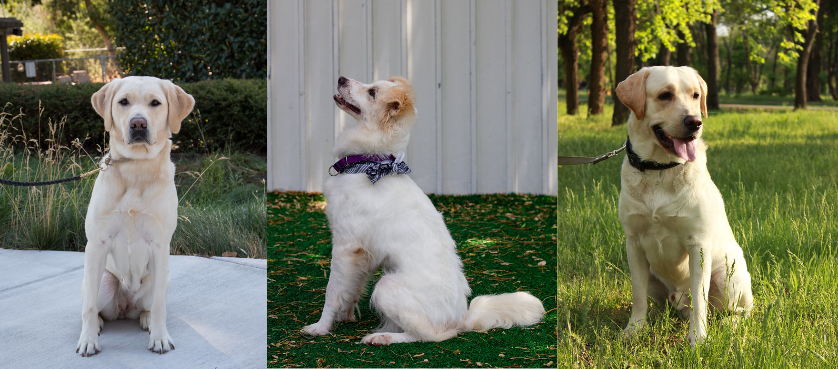
\includegraphics [width=\textwidth] {front_side_view_dog}
  \caption{Cобака в профиль, анфас и 3/4} 
  \label{img:front_side_view_dog}  
\end{figure}

Для отслеживания базовой активности собак нам подойдут оба эти варианта. Возможно отслеживать координаты каждой конечности собаки - лап, хвоста, туловища, головы. Такая задача в иностранной литературе будет называться Pose Estimation. Она подразумевает определение координат конечностей на кадре. 

Так как конечная цель этой работы - классифицировать простые активности собаки, например, когда собака сидит, стоит или лежит - задачу Pose Estimation решать необязательно, но она может значительно упростить дальнейшую классификацию, так как позволит отбросить избыточную визуальную информацию, которую мы имеем на фотографии и оставить только информацию о расположении конечностей относительно друг друга.


\section{Эмоции собак} \label{emotions}
%Section start
% Изначальная миссия этого исследования, выходящего за рамки данной работы, анализировать эмоции собаки. Но для понимания даже базовых эмоций требуется уметь считывать базовые сигналы как поджатый, или наоборот, торчащий хвост. Либо оскал,  

Большинство людей интуитивно понимает основные значения телодвижений собаки и может определить, когда их собака счастлива, напугана или зла. Тем не менее язык тела человека и язык тела собаки очень различаются. Поза, выражение морды и телодвижения, которые мы интерпретируем как определенные эмоции, для вашей собаки могут означать нечто иное. По сути, язык тела собаки состоит из множества различных элементов, которые включают:

\begin{itemize}
    \item Выражение морды.
    \item Положение ушей.
    \item Положение и движение хвоста.
\end{itemize}

Эти аспекты всегда следует интерпретировать вместе, так как это единственный способ точно «расшифровать» эмоции вашей собаки.


\subsubsection{Хвост и уши собаки: выражение эмоций}

Собака сообщает о своих эмоциях и намерениях определенными телодвижениями, будь то общее поведение животного или движения определенной части тела. Однако хвост и уши собаки — это две части тела, на которые следует обращать особое внимание для понимания языка тела животного.\cite{DogSignals}

\subsection{Собачий хвост}

%фотография с разными хвостами: круглый, короткий, длинный. Например, хаски, корги и хз
Как это часто бывает с животными, хвост каждой отдельной собаки говорит о чем-то своем. У некоторых собак хвосты большие и пушистые, у других — хвосты скручены в кольцо и лежат на спине, у третьих — хвосты куцые и мало о чем могут рассказать. Собаки таких пород, как уиппет, ирландский волкодав или борзая, обычно держат хвосты между ног, а значит, они не станут выражать волнение, пряча свои хвосты, как это делают собаки большинства пород. При интерпретации сигналов, подаваемых хвостом, важно всегда учитывать контекст, а также характер и породу отдельной собаки!

\subsubsection{Виляние хвостом}
Одним из самых широко известных является факт, что, виляя хвостом, собака выражает свою радость. Однако в действительности виляние хвостом — не всегда верный признак радости животного. Такое поведение лишь означает, что собака заинтересована во взаимодействии, и только в сочетании с другими элементами языка тела виляние хвостом может быть интерпретировано как радость или беспокойство.

Скорость, с которой собака виляет хвостом, также может послужить ключом к разгадке ее эмоций. Например, быстрое и бодрое виляние обычно является хорошим, дружелюбным жестом, в то время как медленное виляние может быть признаком того, что собака насторожена и взволнована.

\subsubsection{Виляние напряженным хвостом}
Если ваш пес напряжен и скованно виляет хвостом из стороны в сторону, это может быть признаком агрессивного поведения или беспокойства. Иногда это называют «хвост флажком» (не путать с английским термином «флагинг», означающим другое движение хвостом), и он является показателем течки у сук.

\subsubsection{Хвост, зажатый между ног}

%фотка спрятанного хвоста
\begin{figure}[ht] 
  \center
  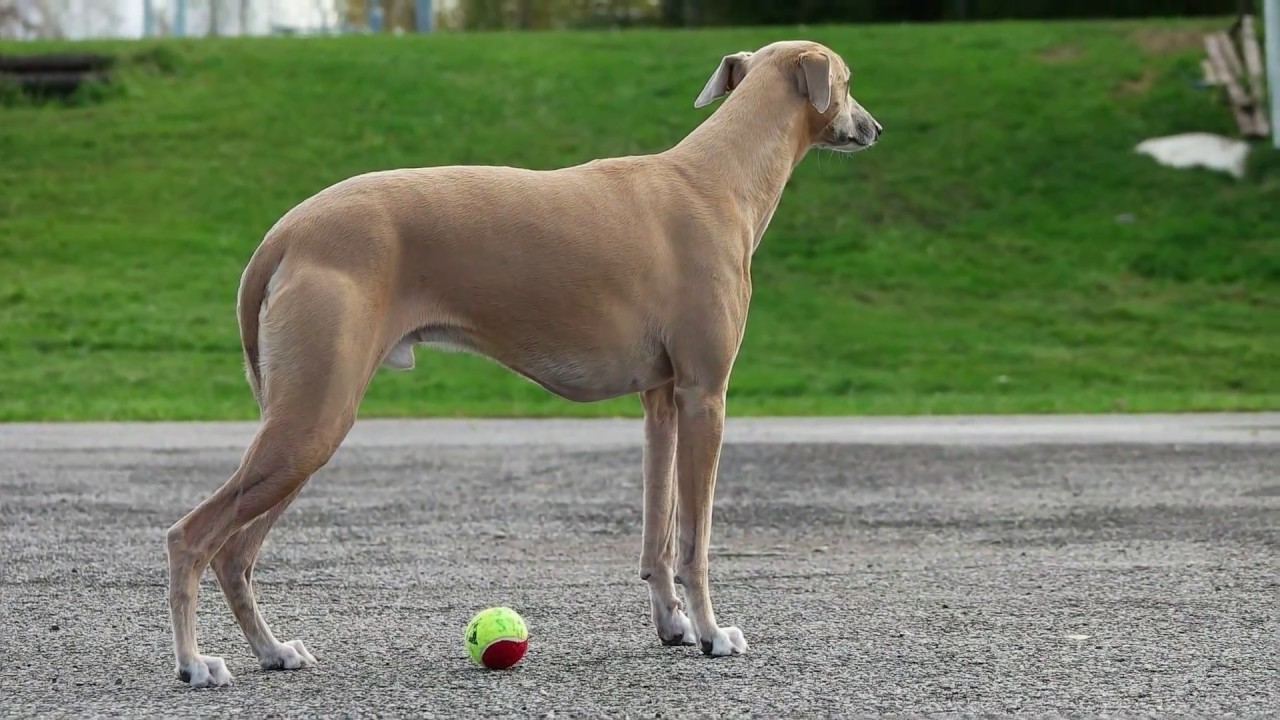
\includegraphics [width=\textwidth/2] {tail-between-legs}
  \caption{Хвост, зажатый между ног} 
  \label{img:tail-between-legs}  
\end{figure}

Если хвост собаки зажат между задними лапами, это означает, что она обеспокоена или напугана. В зависимости от внешних обстоятельств, позы и языка тела собаки, такое поведение может перерасти в оборонительную агрессию, поэтому в подобной ситуации важно подходить к собаке спокойно и осторожно.

Тревожные и пугливые собаки прячут хвост между ног, когда они находятся в незнакомой для них среде или встречают новых людей или животных. Обычно это признак их неуверенности и беззащитности. Послушная собака чаще держит хвост между ног, особенно когда она общается с другими собаками или хочет показать готовность подчиняться, например, в ситуации, когда ее привели к ветеринару на обследование, или после того, как она в чём-то провинилась.

\subsection{Собачьи уши}
\begin{figure}[ht] 
  \center
  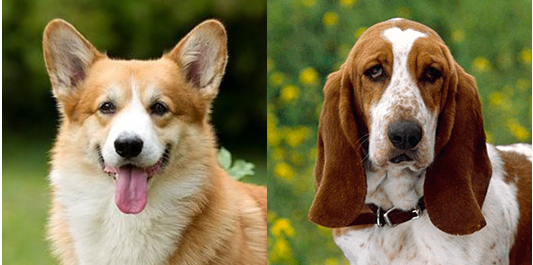
\includegraphics [width=\textwidth/2] {ears-different}
  \caption{У некоторых пород уши острые, у других свисающие} 
  \label{img:ears-different}  
\end{figure}
%кроп ушей острых у корги и бассет-хаунда
Как и в случае с хвостами, форма и тип ушей собаки имеют большое значение в том, как она будет их держать при общении. Не стоит ожидать от собак, например, породы бассет-хаунд, что они будут держать свои уши в вертикальном положении, как это делают породы собак с оттопыренными ушами. В то же время, независимо от формы, размера и типа ушей собаки, можно многое узнать о ее эмоциях и намерениях, научившись распознавать значение положения ушей питомца.

\subsubsection{Уши, направленные назад}
%найти такую фотку
Если уши собаки слегка направлены назад и при этом она радостно виляет хвостом, значит, собака настроена дружелюбно. Однако, если уши плоские и прижаты к спине или по бокам головы, собака определенно сигнализирует о страхе. В зависимости от языка тела собаки с прижатыми ушами ее поведение можно интерпретировать как выражение покорности или наоборот, предупреждение о возможном нападении.

\subsubsection{Заостренные уши}
Всякий раз, когда собака испытывает любопытство или настороженность, она поднимает уши вверх, после чего нередко задирает голову. Более того, собаки слегка направляют уши в сторону объекта или человека, который пробудил в них любопытство.

\subsection{Чтение языка тела собаки}

Язык тела собаки нельзя понять правильно, если при его интерпретации также не учитывать контекст и другие сигналы собаки. Например, оскал может означать радость, подчинение или агрессию — все зависит от остальных элементов языка тела.

Вот некоторые распространённые сигналы, которые обычно передают собаки.

\subsubsection{Выражения морды}

\textbf{Зевание}. Оказывает успокаивающее действие. Если собака не собирается вздремнуть, зевота может указывать на то, что она испытывает стресс или хочет избавиться от переживаний.

\textbf{Взгляд, опущенный вниз}. Собаки не особо любят прямой зрительный контакт, однако если они прожили с людьми долгое время, то начинают понимать, что взгляд не обязательно означает вызов. Отводя глаза, собака, в соответствии с собачьими привычками, просто пытается быть вежливой.

\textbf{Широко раскрытые глаза}. Когда собака отводит взгляд в сторону, концентрируя его на ком-то или чем-то, и виднеются белки (склеры) ее глаз, это признак встревоженности и беспокойства. 

\textbf{Открытый рот}. Такой растерянный вид означает, что пес доволен и расслаблен. Однако, если рот собаки открыт, когда рядом кто-то ест, это может быть просьба поделиться едой.
\begin{figure}[ht] 
  \center
  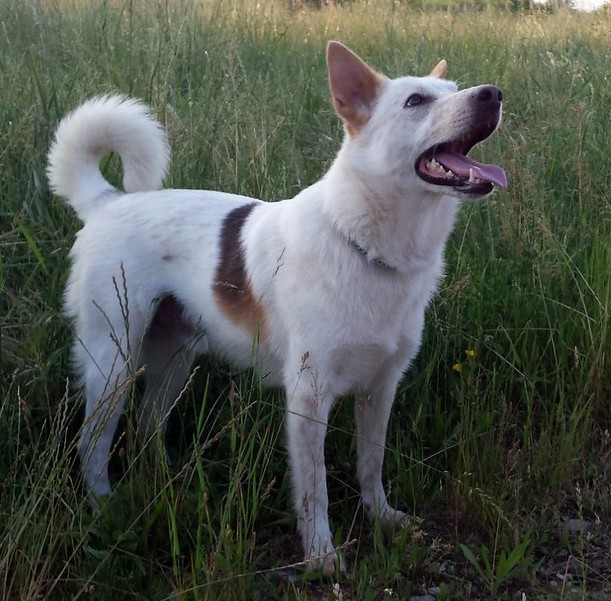
\includegraphics [width=\textwidth/2] {open-mouth}
  \caption{Открытый рот} 
  \label{img:open-mouth}  
\end{figure}
% две фотки тут

\textbf{Оскал / обнаженные зубы}. Этот сигнал может интерпретироваться по-разному в зависимости от ситуации. Он может быть проявлением покорности собаки или, если сопровождается рычанием, поднятой шерстью и защитной стойкой, признаком агрессивных намерений.

\textbf{Облизывание губ}. Если собака постоянно облизывает губы, не глядя при этом на еду, то таким образом она пытается передать чувство страха, стресса или нервозности. Собака может быть напугана или чувствует себя неуютно. В подобной ситуации это также может быть выражено другими сигналами, такими как учащенное дыхание, зажатый между ног хвост или широко раскрытые глаза.

\subsubsection{Положение тела собаки}
% на каждую секцию по фотке
\textbf{Расслабленное}. Расслабленность собаки можно определить, посмотрев на ее тело. Положение ее хвоста будет естественным, положение тела — непринужденным, а уши будут расслаблены или слегка направлены вверх. Собака не станет пристально смотреть или опускать глаза, а ее пасть будет расслаблена в уголках, челюсти сомкнуты или слегка приоткрыты.

\textbf{Возбужденное}. Собака быстро приближается к человеку или объекту, часто переходит на бег, прыжки и демонстрирует игривое настроение. При этом ее уши насторожены и подняты вверх, а хвост не успокаивается. Если пес чем-то особенно взволнован, он может также начать лаять или скулить.

\begin{figure}[ht] 
  \center
  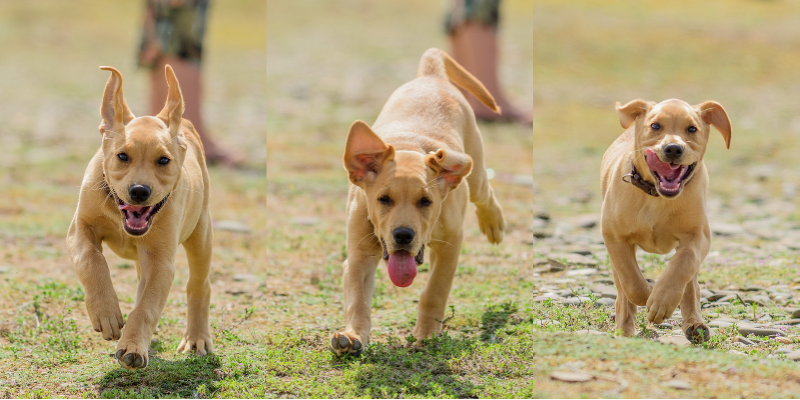
\includegraphics [width=\textwidth*2/3] {dog-run}
  \caption{Собака бежит в игривом настроении} 
  \label{img:dog-run}  
\end{figure}

\textbf{Напуганное}. Есть много способов, с помощью которых собака сообщает о страхе, и все они зависят от характера вашего питомца. Когда собаке страшно, она может нападать, прятаться и проявлять покорное поведение, а также искать утешения у своего хозяина. Большинство собак дрожит, прижимает тело к земле и зажимает хвост между ног.

\textbf{Игривое}. Собаку, которая хочет повеселиться, легко заметить. Типичная игривая стойка, когда передняя часть тела опущена на землю, а задние лапы выпрямлены, является недвусмысленным приглашением к игре как для хозяина, так и для другой собаки.

\textbf{Напряженное}. Если собака чувствует себя неуютно, она подаст об этом знак, напрягая и слегка опуская свое тело, а также направляя уши назад. У некоторых собак напряженная поза сопровождается зеванием или учащенным дыханием.

\textbf{Агрессивное}. Когда собака готовится к нападению, весь язык ее тела демонстрирует такое намерение. Агрессивные собаки имеют сосредоточенный или суженный взгляд, их тело напряжено, шерсть на затылке стоит дыбом, зубы обнажены в оскале, и можно услышать рычание. Тревожный лай и низкое рычание часто сопровождают агрессивное поведение собаки.

\section{Машинное обучение} \label{ML}
Машинное обучение предполагает построение математических моделей, помогающих понять данные. "Обучение" вступает в игру, когда мы даем этим моделям настраиваемые параметры, которые могут быть адаптированы к наблюдаемым данным; таким образом, программу можно считать " обученной" на основе данных. После того, как эти модели подогнаны под ранее наблюдаемые данные, их можно использовать для прогнозирования и понимания аспектов вновь наблюдаемых данных.

\subsubsection{Категории машинного обучения}\label{ml}
На самом фундаментальном уровне машинное обучение можно разделить на два основных типа: обучение с учителем и без него.

%здесь график с методами машинного обучения

Обучение с учителем включает в себя некое моделирование взаимосвязи между измеряемыми характеристиками данных и некоторой маркировкой, связанной с данными; после определения этой модели она может быть использована для нанесения меток на новые, неизвестные данные. Далее это подразделяется на задачи классификации и регрессионные задачи: в классификации метки являются дискретными категориями, а в регрессии - непрерывными величинами. 

% side by side регрессия и классификация

Обучение без учителя включает в себя моделирование свойств данных без привязки к какой-либо метке, и часто описывается как "позволить данным говорить самим за себя". Эти модели включают такие задачи, как кластеризация и уменьшение размерности. Алгоритмы кластеризации идентифицируют различные группы данных, в то время как алгоритмы уменьшения размерности ищут более сжатые представления данных.

% кластеризация

Кроме того, существуют так называемые методы с частичным привлечением учителя, которые находятся где-то между обучением под наблюдением и обучением без наблюдения. Методы с частичным привлечением учителя часто бывают полезны, когда метки имеются лишь для части данных.


\subsection{Нейронные сети} \label{neuralnets}
Попытки воспроизвести способность биологических нервных систем обучаться и исправлять ошибки привели к созданию искусственных нейронных сетей. Искусственные нейронные сети представляют собой семейство моделей, построенных по принципу организации и функционирования биологических нейронных сетей — сетей нервных клеток живого организма.


Понятие искусственной нейронной сети было предложено ещё в 1943 году У. Маккалоком и У. Питтсом в статье \cite{neural_nets}. В частности, ими была предложена модель искусственного нейрона.
Чтобы отразить суть биологических нейронных систем, искусственный нейрон строится следующим образом. Он получает входные сигналы (исходные данные либо выходные сигналы других нейронов нейронной сети) через несколько входных каналов. Каждый входной сигнал проходит через соединение, имеющее определенный вес. С каждым нейроном связано определенное пороговое значение. Вычисляется взвешенная сумма входов, из нее вычитается пороговое значение и в результате получается величина активации нейрона . Сигнал активации преобразуется с помощью функции активации и в результате получается выходной сигнал нейрона.
На Рис.\ref{neuron} приведен пример искусственного нейрона.

\begin{figure}[h]
    \centering
    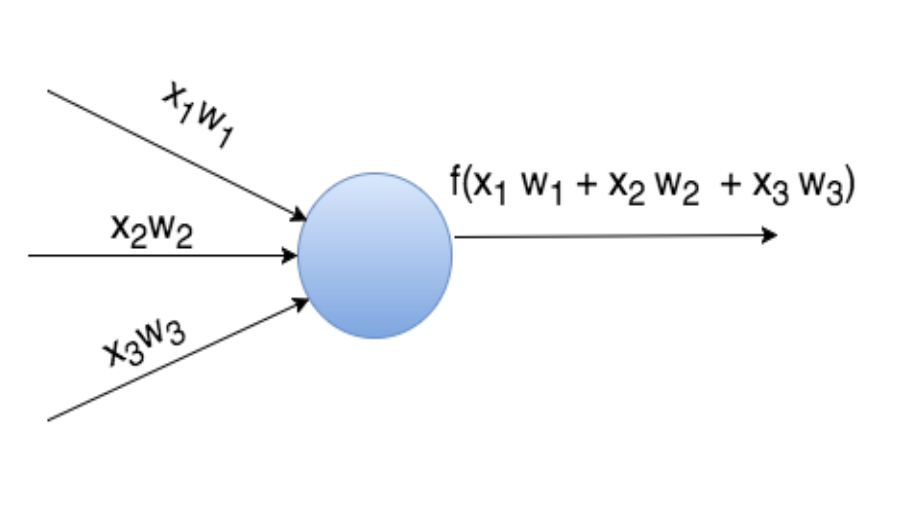
\includegraphics [width=\textwidth*2/3] {images/neuron.png}
    \caption{Искусственный нейрон}
    \label{fig:neuron}
\end{figure}

$x_i$ - входной сигнал
$w_i$ - вес входного сигнала $f(*)$- функция активации

\subsubsection{Функции активации}
В данном разделе описаны используемые в работе функций активаций для нейонных сетей.
\begin{itemize}
    \item Сигмоидная: $f(x) = \dfrac{1}{1-e^{-x}}$
    \item Линейная: $f(x) = x$
    \item Положительно линейная (ReLU): $f(x) = max(0, x)$
    \item  Софтмакс (Softmax): $f(x)j = \dfrac{e^{s_j}}{\sum^K_{k=1}e^{s_k}}$, для $j = 1, .., K$
\end{itemize}

\subsubsection{Функция потерь}
Введем обозначения: $X$— множество описаний объектов, $Y$ — множество допустимых ответов. Предполагается, что существует неизвестная целевая зависимость — отображение $y* : X \rightarrow Y$ , значения которой известны только на объектах конечной обучающей выборки 
$X^m = \begin{matrix}\{ (x_1, y_1), & ..., & (x_m, y_m)  \}\end{matrix}$.

Вводится функция потерь $L(y, y')$, характеризующая величину отклонения ответа $y$ от правильного ответа $y' = y^*(x)$ на произвольном объекте $x \in X$. Тогда эмпирический риск \cite{classification} — функционал качества, характеризующий среднюю ошибку на обучающей выборке:
\[
    Q(a,X^m)= \dfrac{1}{m} \sum^m_{i=1} L(y_i,y^*(x_i))
\]
В процессе обучения нейронная сеть настраивает веса $W$, минимизируя эмпирический риск.

При решении задачи многоклассовой классификации на выходе нейронной сети необходимо получить вероятность принадлежности объекта каждому из классов. В этом случае в качестве функции потерь обычно используется перекрёстная энтропия или кросс-энтропия

\[
L(y, y^*(x_i)) = -\sum^K_{j=1}y^*_{ij} \log y_{ij}
\]
где $K$ - количество меток классов в задаче.
 
\subsection{Свёрточные нейронные сети} \label{convnets}
С появлением больших объемов данных и больших вычислительных возможностей стали активно использоваться нейронные сети. Особую популярность получили сверточные нейронные сети, архитектура которых была предложена Яном Лекуном \cite{LeCun1998GradientbasedLA} и нацелена на эффективное распознавание изображений. Свое название архитектура сети получила из-за наличия операции свёртки, суть которой в том, что каждый фрагмент изображения умножается на матрицу (ядро) свёртки поэлементно, а результат суммируется и записывается в аналогичную позицию выходного изображения. 

В архитектуру сети заложены априорные знания из предметной области компьютерного зрения: пиксель изображения сильнее связан с соседним (локальная корреляция) и объект на изображении может встретиться в любой части изображения.

Особое внимание свёрточные нейронные сети получили после конкурса ImageNet\cite{imagenet}, который состоялся в октябре 2012 года и был посвящен классификации объектов на фотографиях. В конкурсе требовалось распознавание образов в 1000 категорий. Победитель данного конкурса - Алекс Крижевский, используя свёрточную нейронную сеть, значительно превзошел остальных участников\cite{alexnet}.

\subsection{Архитектура свёрточной нейронной сети} \label{cnnarch}
Сверточная нейронная сеть обычно представляет собой чередование сверточных слоев (convolution layers), субдискретизирующих слоев (subsampling layers), при наличии полносвязных слоев (fully-connected layer) на выходе. Все три вида слоев могут чередоваться в произвольном порядке \cite{LeCun1998GradientbasedLA}.

В сверточном слое нейроны, которые используют одни и те же веса, объединяются в карты признаков (feature maps), а каждый нейрон карты признаков связан с частью нейронов предыдущего слоя. При вычислении сети получается, что каждый нейрон выполняет свертку некоторой области предыдущего слоя (определяемой множеством нейронов, связанных с данным нейроном).

Пример архитектуры сверточной нейронной сети представлен на Рис. \ref{fig:convnet}.
\begin{figure}[h]
    \centering
    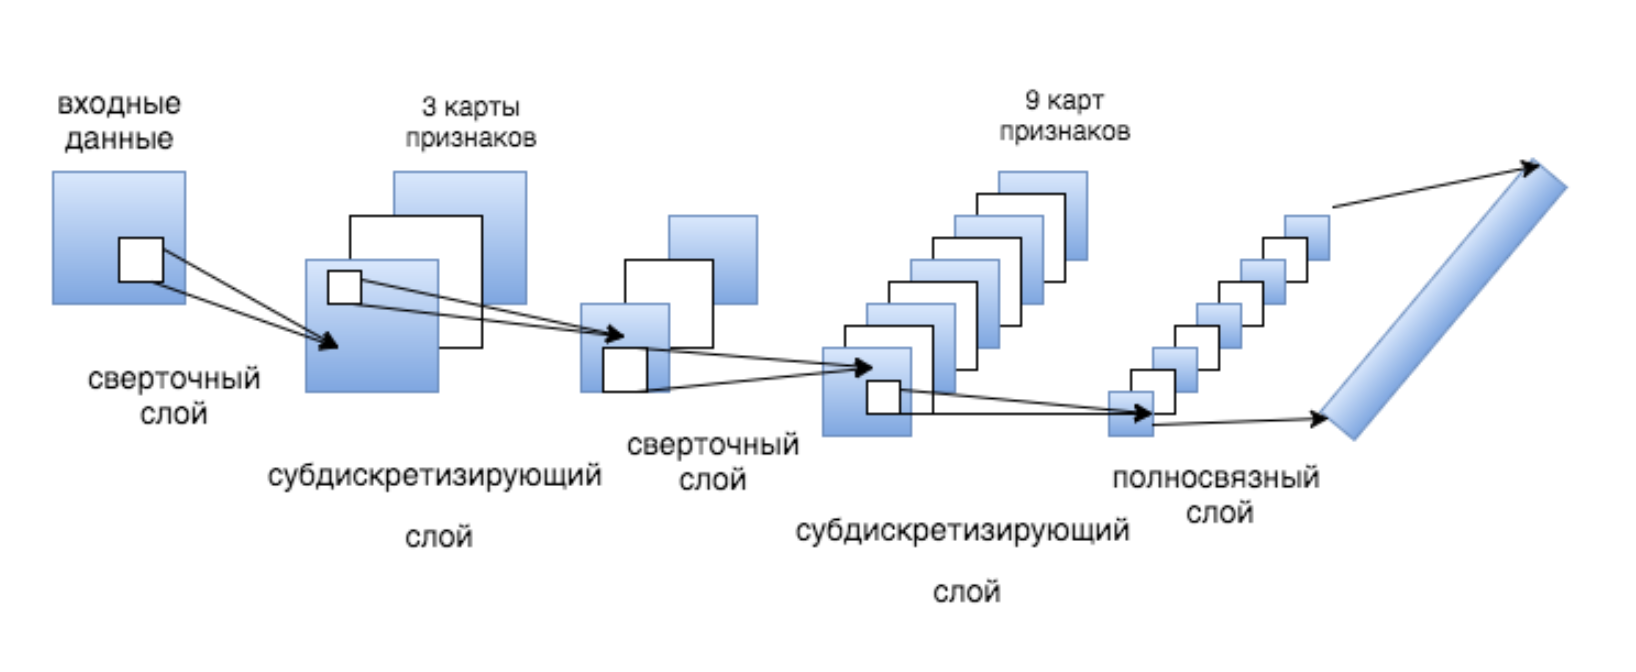
\includegraphics [width=\textwidth*2/3] {images/convnet.png}
    \caption{ Архитектура сверточной нейронной сети}
    \label{fig:convnet}
\end{figure}

\subsubsection{Полносвязный слой} \label{fc_layers}
Слой в котором каждый нейрон соединен со всеми нейронами на предыдущем уровне, причем каждая связь имеет свой весовой коэффициент. На Рис.\ref{fig:fc_layer} показан пример полносвязного слоя.

\begin{figure}[h]
    \centering
    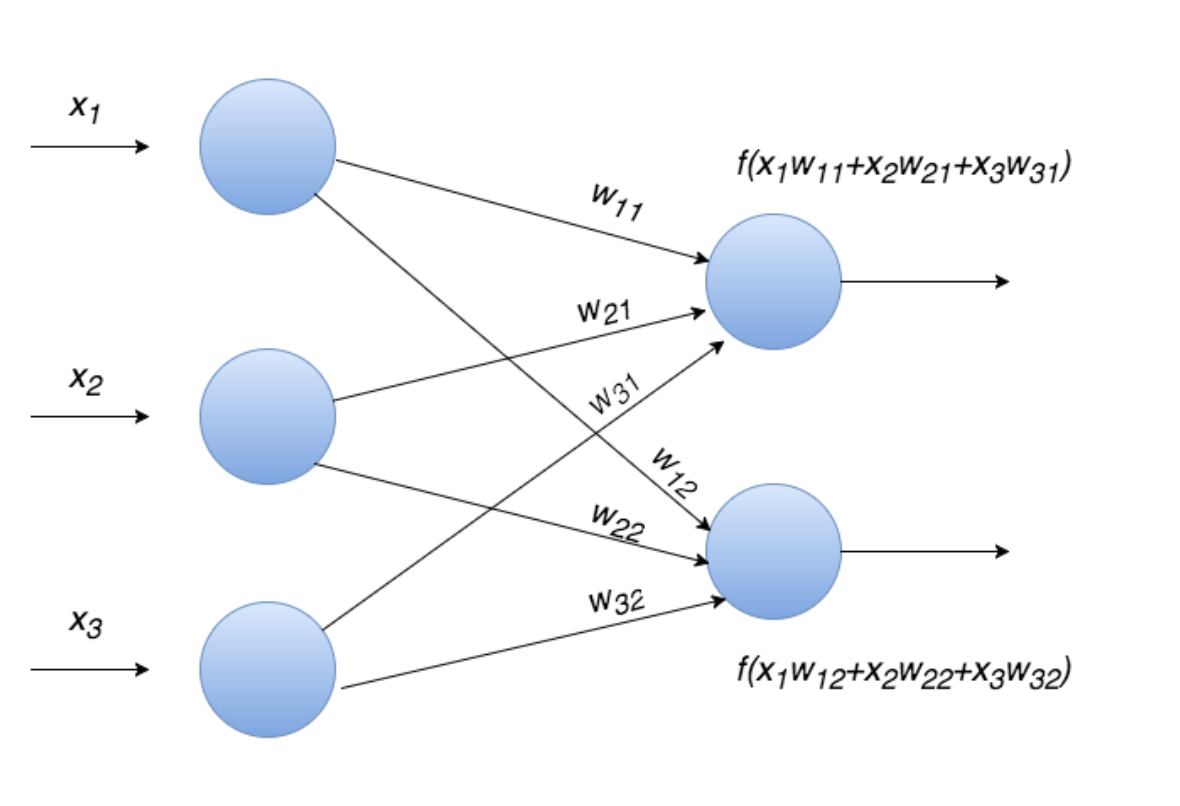
\includegraphics [width=\textwidth*2/3] {images/fc_layer.png}
    \caption{Полносвязный слой}
    \label{fig:fc_layer}
\end{figure}

\begin{itemize}
    \item $w_{i,j}$ — весовые коэффициенты
    \item $f(*)$ — функция активации
\end{itemize}

\subsubsection{Свёрточный слой} \label{conv_layers}
В отличие от полносвязного, в свёрточном слое нейрон соединен лишь с ограниченным количеством нейронов предыдущего уровня, т. е. сверточный слой аналогичен применению операции свертки, где используется лишь матрица весов небольшого размера (ядро свертки), которую «двигают» по всему обрабатываемому слою.

Еще одна особенность свёрточного слоя в том, что он немного уменьшает изображение за счет краевых эффектов.

На Рис. \ref{fig:conv_layer} показан пример сверточного слоя с ядром свертки размера $3 \times 3$.
\begin{figure}[h]
    \centering
    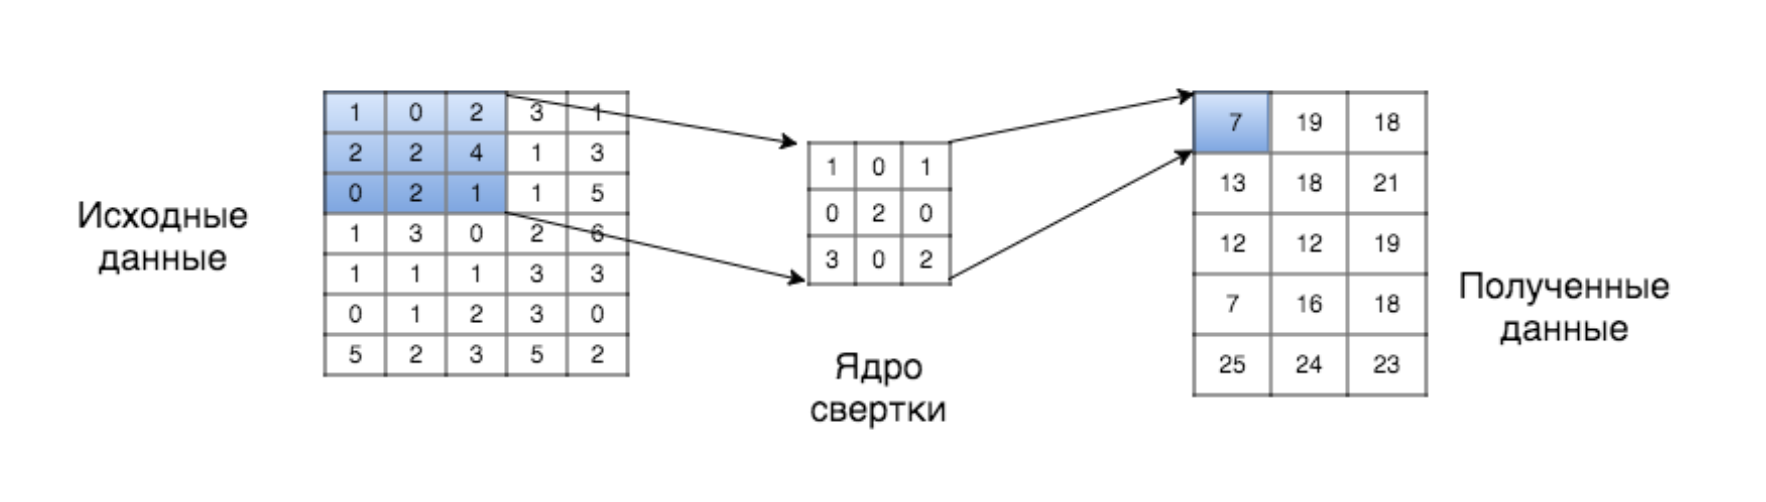
\includegraphics [width=\textwidth*2/3] {images/conv_layer.png}
    \caption{Сверточный слой}
    \label{fig:conv_layer}
\end{figure}

\subsubsection{Cубдискретизирующий слой} \label{pooling_rev}
Слои этого типа выполняют уменьшение размерности (обычно в несколько раз). Это можно делать разными способами, но зачастую используется метод выбора максимального элемента (max-pooling) — вся карта признаков разделяется на ячейки, из которых выбираются максимальные по значению.

На Рис. \ref{fig:pooling_layer} показан пример субдискретизирующего слоя с методом выбора максимального элемента.
\begin{figure}[h]
    \centering
    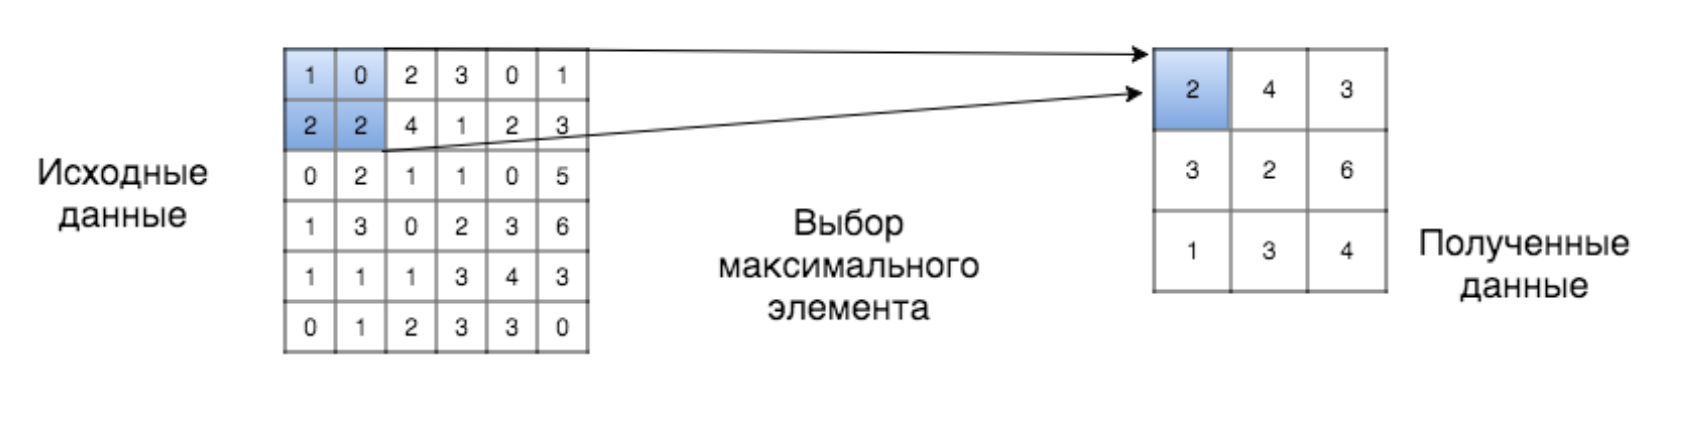
\includegraphics [width=\textwidth*2/3] {images/pooling_layer.png}
    \caption{Cубдискретизирующий слой}
    \label{fig:pooling_layer}
\end{figure}

\subsubsection{Dropout слой} \label{dropout_rev}
Dropout слой (dropout регуляризация)\cite{dropout} способ борьбы с переобучением в нейронных сетях, обучение которых обычно производят стохастическим градиентным спуском, случайно выбирая некоторые объекты из выборки. 

Dropout регуляризация заключается в изменении структуры сети: каждый нейрон выбрасывается с некоторой вероятностью $p$. По такой прореженной сети производится обучение, для оставшихся весов делается градиентный шаг, после чего все выброшенные нейроны возвращаются в нейросеть.

Таким образом, на каждом шаге стохастического градиента мы настраиваем одну из возможных $2N$ архитектур сети, где под архитектурой мы понимаем структуру связей между нейронами, а через $N$ обозначаем суммарное число нейронов. При тестировании нейросети нейроны уже не выбрасываются, но выход каждого нейрона умножается на $(1 - p)$ - благодаря этому на выходе нейрона мы будем получать математическое ожидание его ответа по всем $2N$ архитектурам. Таким образом, нейросеть, обученную с помощью dropout-регуляризации, можно рассматривать как результат усреднения $2N$ сетей.

\subsection{Реализации свёрточных нейронных сетей} \label{nn_archs_lit}
Теперь рассмотрим архитектуры нейронных сетей, которые будут использоваться далее в работе.

\subsubsection{ResNet} \label{resnet_rev}

В 2015 году ResNet произвела настоящую революцию глубины нейросетей. Она состояла из 152 слоёв и снизила процент ошибок до 3,57\%\cite{resnet} в соревновании классификации ImageNet.

Что происходит с нейросетью, при увеличении количества слоёв? Можно ли, взяв обычную архитектуру как AlexNet, просто складывать всё больше и больше слоёв друг на друга и достигать лучшей точности? 

Авторы ResNet в статье описали, что нельзя. Скорее всего, более глубокая нейросеть покажет даже худшие результаты как при обучении, так и при тестировании. И это будет не из-за переобучения, поскольку тогда тренировочная ошибка была бы низкой, см Рис \ref{fig:train_error_deep_net}.

\begin{figure} [h]
    \centering
    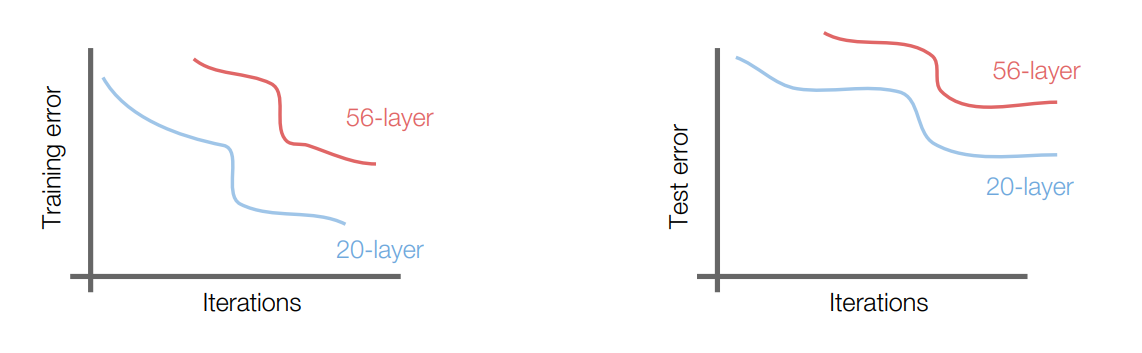
\includegraphics[width=\textwidth*2/3]{images/train_error_deep_net.png}
    \caption{Ошибка на обучающей и тестовой выборке у сети с 20 слоями и 56 слоями}
    \label{fig:train_error_deep_net}
\end{figure}

Создатели ResNet предположили, что узкое место глубоких нейронных сетей кроется в оптимизации — более глубокие модели гораздо хуже поддаются настройке. Тогда они решили не складывать слои друг на друга для изучения отображения нужной функции напрямую, а использовать остаточные блоки, которые пытаются «подогнать» это отображение. Так ResNet стала первой остаточной нейронной сетью\cite{resnet}. Говоря простыми словами, она «перепрыгивает» через некоторые слои. Они больше не содержат признаков и используются для нахождения остаточной функции $H(x) = F(x) + x$ вместо того, чтобы искать $H(x)$ напрямую.

\begin{figure}
    \centering
    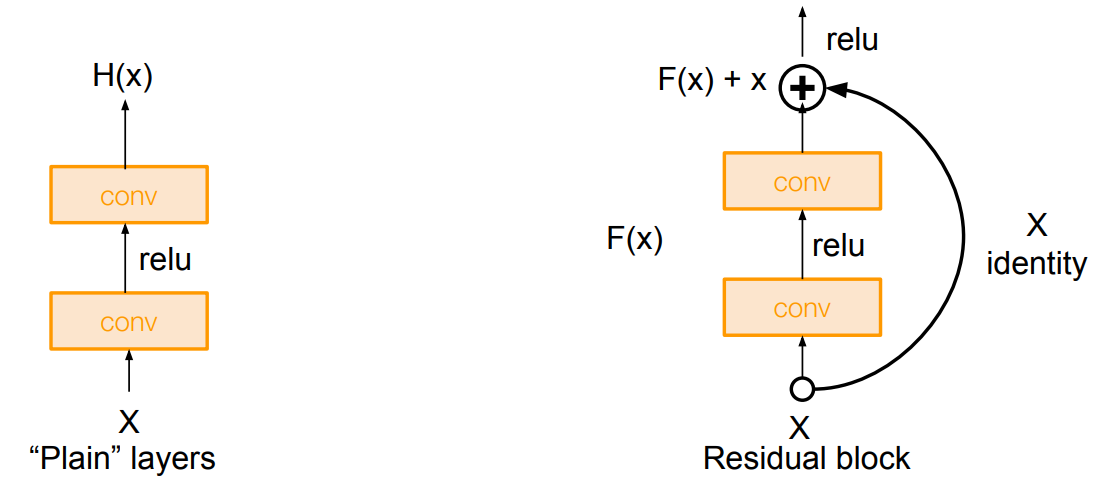
\includegraphics[width=\textwidth*2/3]{images/res_block.png}
    \caption{Обычный слой свёртки и остаточный блок у ResNet}
    \label{fig:my_label}
\end{figure}


Нейросеть состоит из большого стека одинаковых остаточных блоков, каждый из которых имеет два свёрточных слоя $3 \times 3$. Периодически число фильтров удваивается, а их размерность уменьшается с шагом 2 (2 в каждом измерении). В самом начале архитектуры присутствует дополнительный свёрточный слой. Также у ResNet нет полносвязных слоёв в конце — используется только один слой с выходными классами.

Параметры обучения нейронной сети:
\begin{itemize}
    \item После каждого свёрточного слоя используется пакетная нормализация.
    \item SGD + Momentum 0.9.
    \item Скорость обучения — 0.1, делится на 10 при затухании скорости изменения ошибки.
    \item Размер мини-пакета — 256.
    \item Затухание весов — 1e-5.
    \item Dropout не используется.
\end{itemize}

В результате экспериментов с ResNet выяснилось, что очень глубокие сети действительно можно обучить без ухудшения точности. Нейросеть достигла наименьшей ошибки в задачах классификации, которая превзошла даже человеческий результат.

\subsubsection{MobileNet} \label{mobilenet_rev}
В 2017 году Google создала целый класс эффективных моделей под названием MobileNets для мобильных и встраиваемых приложений технического зрения. Сети MobileNet основаны на легковесной архитектуре, использующей разделяемые по глубине свёртки для построения легких глубоких нейронных сетей. 

Нейронная сеть обладает двумя простыми глобальных гиперпараметрами, которые позволяют выбирать между скоростью вычислений и точностью. Эти гиперпараметры позволяют выбрать правильный размер модели для своего приложения, основываясь на ограничениях проблемы. 

Архитектура демонстрирует высокую производительность по сравнению с другими популярными моделями по классификации ImageNet. Спектр применения включает в себя обнаружение объектов, классификацию, распознавание лиц и крупномасштабную геолокализацию.\cite{mobilenet}

Основная особенность этой архитектуры заключается в наличии операторов сгруппированной свёртки. Она позволяет значительно сократить количество вычислений и параметров у модели \cite{xception}. Рассмотрим этот оператор свёртки более подробно.

Сгруппированная свертка - это вариант свертки, при котором каналы карты входных признаков сгруппированы, а свертка выполняется независимо для каждого сгруппированного канала. Её пример можно увидеть на рисунке \ref{fig:gconv}.

\begin{figure}[h]
    \centering
    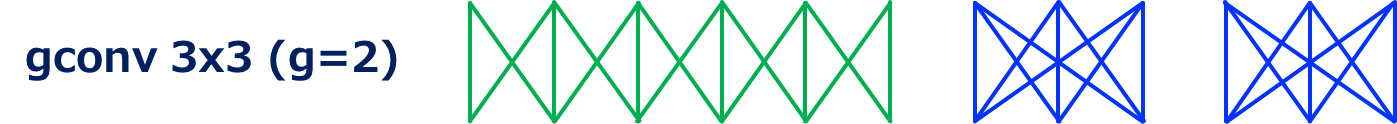
\includegraphics[width=\textwidth*2/3]{images/gconv.png}
    \caption{Сгруппированная свёртка на 5 слоях}
    \label{fig:gconv}
\end{figure}

По сравнению с обычной свёрткой, на рисунке \ref{fig:normal_conv}, можно увидеть что на группированной свёртке слои, разбиваются на две группы, и количество перемножений разительно падает.

\begin{figure}[h]
    \centering
    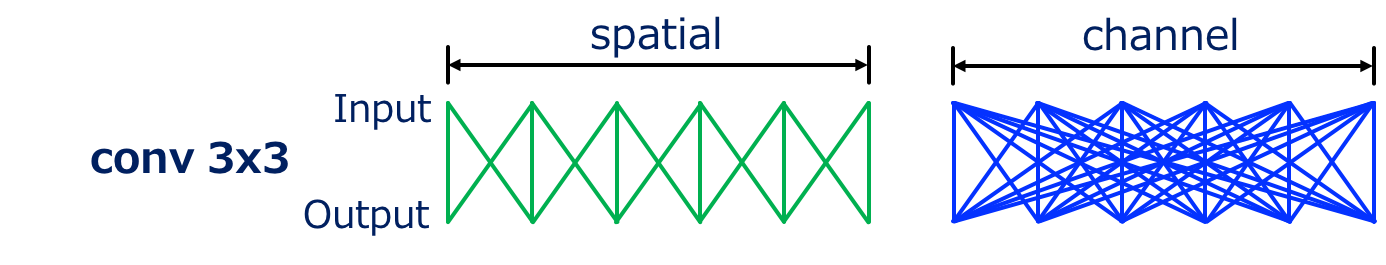
\includegraphics[width=\textwidth*2/3]{images/normal_conv.png}
    \caption{Обычная свёртка на 5 слоях}
    \label{fig:normal_conv}
\end{figure}

Количество вычислений при обычной свёртке:
\[
    Cost = HWNK^2M
\]

где
\begin{itemize}
    \item $Cost$ - Computational Cost или количество вычислений
    \item $H$ - высота изображения
    \item $W$ - высота изображения
    \item $N$ - количество каналов на входе
    \item $K$ - размер ядра свёртки. В квадрате, т.к. высота и ширина ядра обычно равны
    \item $M$ - количество каналов на выходе
\end{itemize}

При сгруппированной свёртке количество вычислений падает пропорционально количеству групп. 
\[
    Cost = \dfrac{HWNK^2M}{G}
\]

где $G$ - это количество групп свёртки.

Когда количество групп свёртки совпадает с количеством слоёв в исходном изображении, такую свёртку называют depthwise convolution или послойная свёртка. Рис \ref{fig:depthwise_conv}.

\begin{figure}[h]
    \centering
    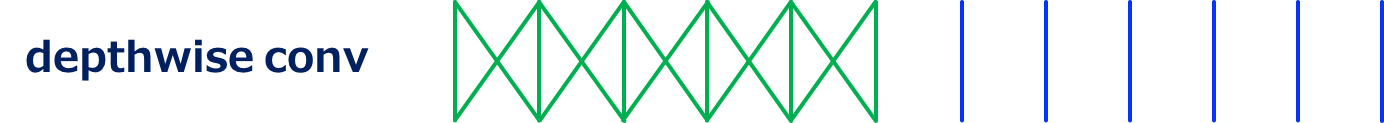
\includegraphics[width=\textwidth*2/3]{images/depthwise_conv.png}
    \caption{Послойная свёртка}
    \label{fig:depthwise_conv}
\end{figure}


\section{Существующие датасеты} \label{datasets}
Насколько известно автору, по состоянию на Май 2020 года в открытом доступе содержатся только следующие наборы данных с изображениями собак:
\begin{enumerate}
  \item ImageNet \cite{imagenet} - Считается крупнейшим датасетом по классификации всего. Насчитывает более 1 миллиона изображений и больше 1000 классов изображений для классификации, начиная от машин, заканчивая собаками. Часто используется для оценки производительности систем компьютерного зрения а также для предобучения нейронных сетей при недостаточных данных.
  \item Stanford Dog Dataset \cite{KhoslaYaoJayadevaprakashFeiFei_FGVC2011} - Подраздел ImageNet. В нём содержится 20000 изображений собак 120 различных пород. Разметка осуществлялась для дальнейшей классификации собак по породам. Разные породы имеют различное количество изображений.
  \item OpenImageDataset \cite{openimages} - ближайший аналог ImageNet по назначению и реализации, за тем лишь исключением что он создавался с уклоном в детекцию объектов, поэтому все изображения там чуть большего размера, и на каждом изображения может быть несколько объектов, в том числе, разного класса. К каждому объекту прилагается информация о его ограничивающей рамке.
  \item DogCentric Activity Dataset \cite{yumi2014first} - Датасет с видеозаписями различных занятий собаки от лица самой собаки. Целью является классификация активности. В видеозаписях видно только затылок и уши собаки.
  \item Jena Action Recognition Dataset \cite{jena} - Коллекция видеозаписей с дистанционно управляемым роботом-собакой SONY ERS-7 Aibo. Создавалась для оценивания систем распозанавания. В ней есть видеозаписи, координаты ограничивающих рамок робота на каждом кадре и данные для калибровки.
\end{enumerate}
Все эти датасеты достаточно хорошо размечены. Важно заметить что в изображения собак в ImageNet, Stanford Dog Dataset и OpenImageDataset пересекаются, так что суммарно по этим трём датасетам имеется всего 20000 изображений собак, столько же сколько и в Stanford Dog Dataset.

\section{Методы решения задачи} \label{methods}

В области определения позы животных проделано сильно меньше работы, чем в этой же области для людей. Причины очевидны:
\begin{itemize}
    \item Широкий потенциал применения
    \item Возможность использовать актёров
    \item Большое количество фотографий
\end{itemize}
\subsection{На людях} \label{subsect1_3_1}
Сейчас классификацию позы людей осуществляют с помощью так называемого Pose Estimation Tree. Целью зрения становится будто восстановить человеческий скелет по изображению. Для этого определяются важные подвижные узлы - joints. Обычно ими являются локти, колени и другие суставы. У человека всего порядка 200 таких узлов. При этом при решении большинства задач компьютерного зрения используется около 20.
\begin{figure}[ht] 
  \center
  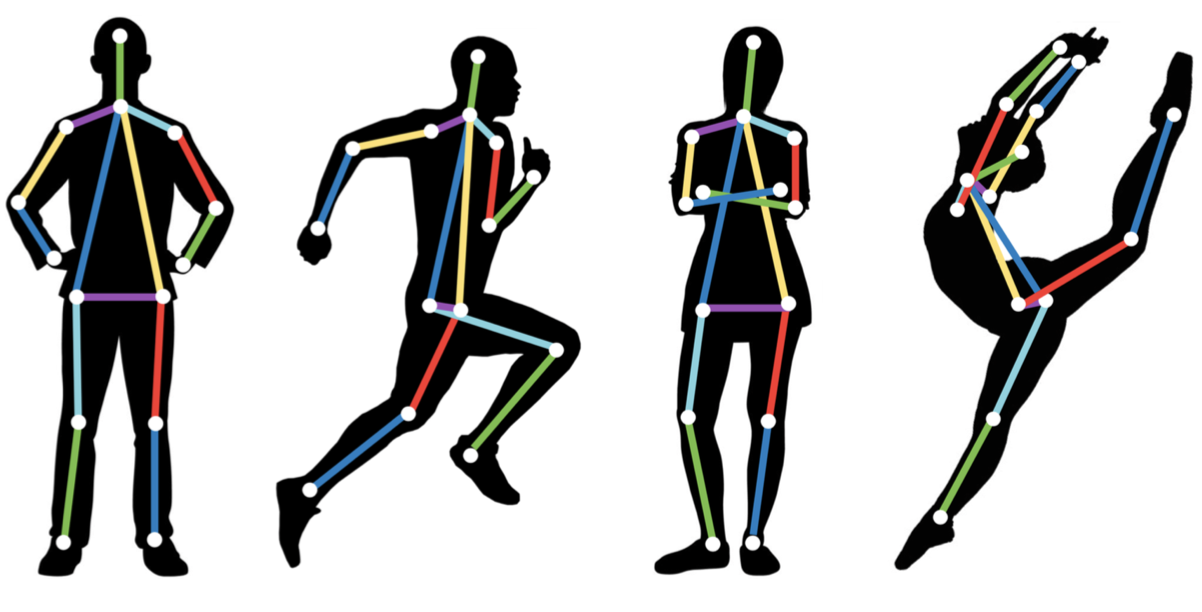
\includegraphics [width=\textwidth/2] {pose}
  \caption{Pose Estimation Tree} 
  \label{img:poseest}  
\end{figure}

Классические пакетные решения для такой задачи - Tensorflow Pose Kit и OpenPose. Всё что требуется для этих пакетов - набор размеченных данных для обучения. OpenPose может работать с множественными объектами и окклюзиями, но относительно медленный. Tensorflow Pose Kit создан с уклоном в перенос модели на портативные устройства.

В статье выпускников Стенфорда 2015 года советуется использовать классификацию деятельности строго отдельно от задачи получения дерева конечностей человека, а не одно на результатах другого.\cite{Bearman2015HumanPE} Основная причина в том, что дерево конечностей крайне нестабильно, его точность далека от идеальной и от окклюзий конечностей самим человеком практически нельзя избавиться. В подтверждение этому, на 20 классах активности, они добились точности в 80\% без использования pose estimation, что считается хорошо для такого большого количества классов.

\subsection{На животных} \label{subsect1_3_2}
В 2018 году вышла публикация \cite{deeplabcut}, в которой авторы предложили новаторский способ автоматически следить за указанными частями тела у животных. Алгоритму не требуется больших датасетов с данными, нужно всего около 200 кадров (от 8 секунд видео) чтобы предсказать остальной видеопоток. 
\begin{figure}[ht] 
  \center
  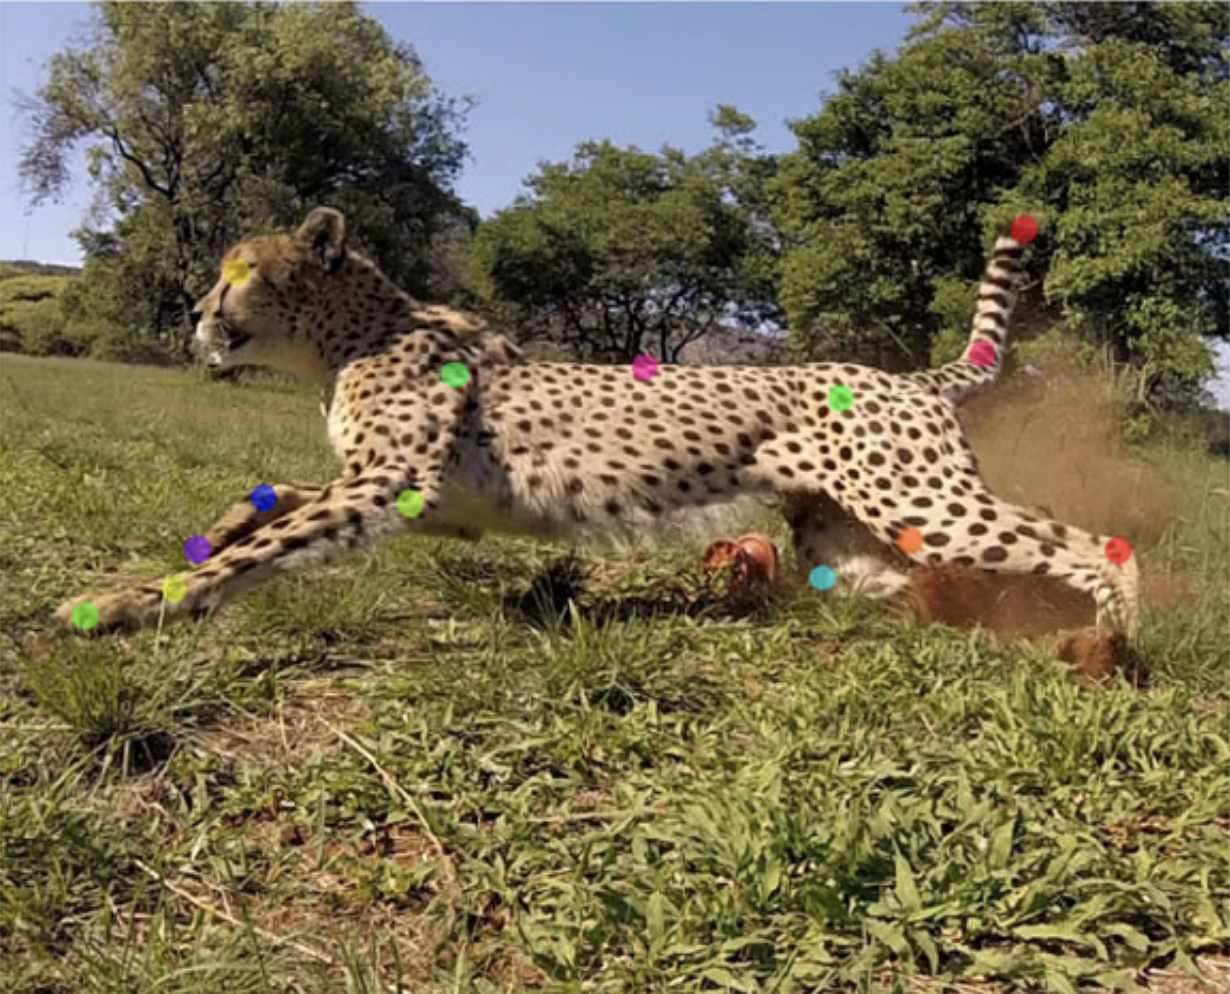
\includegraphics [width=\textwidth/2] {deeplabcut}
  \caption{Предсказанный кадр DeepLabCut} 
  \label{img:deeplabcut}  
\end{figure}
Ограничениями данного метода являются необходимость в разметке этих первых 200 кадров, на это уходит обычно около 20 минут, а также принципиальная возможность работать только с видеопотоком. 
В итоге это достаточно хороший метод для того чтобы разметить большие видеопотоки. Алгоритм обеспечивает достаточную точность и на длинных видеозаписях позволяет сильно сократить время на разметку данных для Pose Tree Estimation. Применение данного способа не ограничивается только на животных: любой видеопоток, на котором можно отслеживать объекты будет работать.


\section{Разметка данных} \label{labeling}
Обязательным процессом любой задачи связанной с машинным обучением является получение и разметка данных. Разметкой данных в зависимости от объёма можно заниматься как самостоятельно, так и с помощью наёмного труда. 

\subsection{Самостоятельная разметка данных} \label{subsect1_3_1}
Нет ничего страшного в том чтобы разметить несколько тысяч изображений. Практика показывает, что на самостоятельную разметку тысячи изображений при наличии необходимых инструментов уходит от 20 минут до часа.

К достоинствам самостоятельной разметки можно отнести:
\begin{itemize}
    \item Надёжность - возможность полностью контролировать результат
    \item Независимость - нет нужды полагаться на других людей или сервисы
    \item Дешевизна - не нужно никому платить
    \item Возможность ознакомится с набором данных
\end{itemize}
И действительно, ознакомившись с набором данных, можно увидеть его недостатки, или наоборот, особенности, которые могут помочь решить задачу.

Недостатки:
\begin{itemize}
    \item Разметка больших наборов данных изнуряет
    \item Это самый медленный способ получить данные
    \item Часто приходится создавать инструменты для разметки самостоятельно
\end{itemize}


\subsection{Разметка данных с помощью сторонних сервисов} \label{subsect1_4_2}
Когда самостоятельная разметка невозможна или занимает слишком много времени, можно воспользоваться специальными сервисами для разметки данных. Такими являются Яндекс.Толока и Amazon Mechanical Turk.

Достоинства:
\begin{itemize}
    \item Скорость - из-за большого количества пользователей на разметку даже больших датасетов редко уходит больше часа.
    \item Встроенные в сервисы инструменты для разметки
    \item Относительная дешевизна.
\end{itemize}
Недостатки:
\begin{itemize}
    \item Качество разметки крайне низкое
    \item Для сложных заданий требуется составлять обучение
    \item Требуется опыт в составлении заданий на платформе
    \item Невозможность разметки коммерчески секретных данных
\end{itemize}
Главным недостатком таких сервисов является то, что пользователи не знают ничего о задаче автора. Поэтому задания надо составлять максимально точно, и заставлять пользователей проходить обучение прежде чем решать задачу. Более того, часть пользователей могут вместо правильных ответов давать быстрые, и за этим тоже необходимо следить.

\subsection{Разметка данных с помощью наёмного штата} \label{subsect1_4_3}
Обычно, серьёзные команды на рынке машинного обучения для разметки данных используют собственные наёмные команды.

Достоинства:
\begin{itemize}
    \item Высокое качество разметки
    \item Возможность получать обратную связь
    \item Возможность лично и устно формулировать задания штату
    \item Возможность подписать соглашение о неразглашении
\end{itemize}
Недостатки:
\begin{itemize}
    \item Цена. Это самый дорогой способ
\end{itemize}
Часто такие команды нанимают под однотипные задачи. Например, если есть постоянный поток данных с камер автомобилей, такая команда может размечать данные специально для компании. В таком случае можно обеспечить постоянную нагрузку на штат, а сотрудники будут опытными в решении задачи.           % Глава 1
\chapter{Постановка задачи} \label{chapt2}

Почти все задачи машинного обучения содержат в себе три важные подзадачи:
\begin{enumerate}
    \item Сбор данных
    \item Обучение нейронной сети
    \item Решение инфраструктурных задач
\end{enumerate}

В данном проекте задача решалась итеративно, и цикл повторяется пока задача не будет считаться решённой. Причина этому - более экономная трата ресурсов и постоянная обратная связь. Если несколько циклов подряд задачу решить не получается - меняют вводные, либо меняют задачу. 

\section{Содержательная} \label{sect2_1}
\textbf{Дано: } 

Изображение или видеопоток, на котором гарантированно присутствует собака.

\textbf{Требуется: } 

Вернуть информацию о позиции собаки в данный на изображении среди следующих классов: [Стоит, сидит, лежит].

Требования к изображению и видеопотоку, которые идут на вход указанной системе. 

Собака в кадре должна быть:
\begin{itemize}
    \item Видна целиком
    \item Ничем не загорожена, даже частично
    \item На кадре находится одна
    \item Занимает более 50\% кадра по высоте или по ширине
    \item Хвост может быть загорожен телом 
    \item От собаки до края кадра есть ещё место, больше 1\% высоты и ширины кадра
 \end{itemize}
 
Камера относительно собаки:
\begin{itemize}
    \item Находится на расстоянии более 2м
    \item Смотрит на собаку на уровне глаз либо выше, но не сверху.
\end{itemize}

Для того чтобы гарантировать присутствие собаки в кадре и тот факт что она одна, будет использоваться другая, отдельная нейронная сеть. 


\section{Математическая} \label{sect2_2}
Данная задача сведена к задаче классификации изображений по N классам. Наличие собаки гарантируется на кадре. Чтобы классифицировать изображение, используется свёрточная нейронная сеть архитектуры ResNet-34 \cite{resnet}.

\begin{figure}[ht] 
  \center
  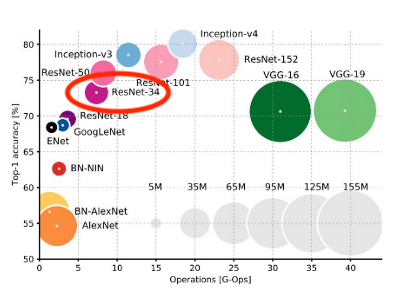
\includegraphics [scale=1] {resnet}
  \caption{Соотношение точности к сложности вычислений у ResNet-34 относительно других архитектур} 
  \label{img:resnet}  
\end{figure}

Для того чтобы гарантировать исполнение условий, указанных в содержательной постановке задачи, используется предобученная нейронная сеть по сегментации изображений MaskRCNN. Она получает на вход изображение и возвращает маску объектов, находящихся на ней. Нас интересуют собаки. Если масок несколько - значит, на кадре больше одной собаки. Если масок собак нет - значит на кадре собак нет. Эти две простые проверки сильно увеличивают качество нейронной сети. Помимо этих проверок, маска позволяет убрать ненужную часть кадра, уменьшая шанс того что нейронная сеть ошибётся.

Также в работе используется MobileNet v2\cite{mobilenet} при работе с маленькими датасетами. Изменения от оригинальной статьи только в так называемой «голове» классификации и размере входного изображения. Структура следующая:

\begin{figure}[ht] 
  \center
  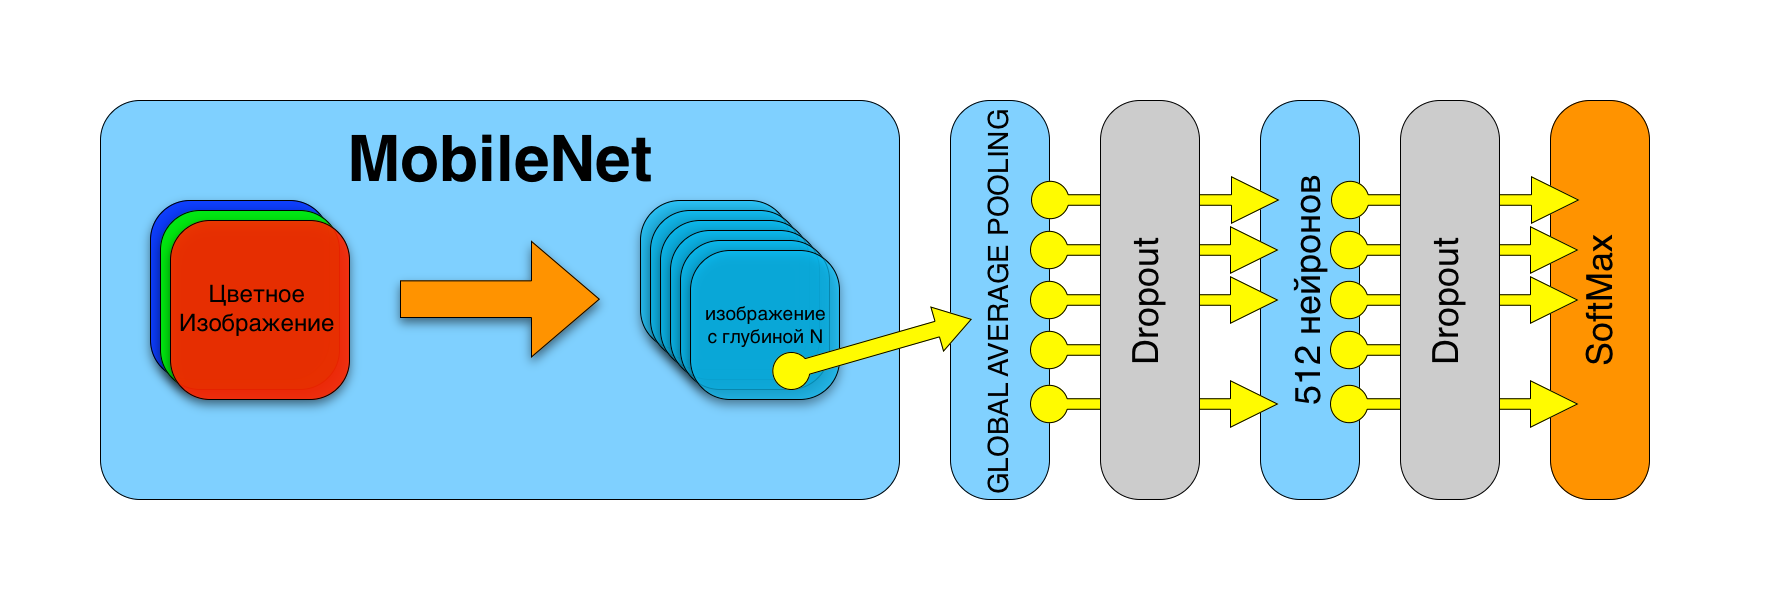
\includegraphics [width=\textwidth] {NN_arch}
  \caption{Архитектура используемой нейронной сети} 
  \label{img:NN_arch}  
\end{figure}

\begin{itemize}
    \item Входное изображение 96х96 пикселей с 3 каналами
    \item Основа MobileNet V2, без "головы"
    \item Global Average Pooling - последняя карта активации(3-мерный тензор) преобразуется в плоский вектор, каждый слой превращается в одно число - среднее по слою. Это позволяет нейронной сети быть инвариантной к размеру входного изображения
    \item Слой DropOut - обнуление 20\% разных значений предыдущего слоя
    \item Batch Norm - нормализация вектора относительно других изображений в мини-партии данных для обучения
    \item Полносвязный слой с 512 нейронами
    \item Функция активации, ReLU
    \item DropOut
    \item BatchNorm
    \item Выходной слой n нейронов, по количеству классов. Функция активации - softmax. 
\end{itemize}

Такая архитектура обусловлена борьбой с переобучением нейронной сети на маленьких объёмах данных. Размер входного изображения держался на минимальном уровне, обычно нейронные сети используют по 224 пикселя по длине и ширине, здесь же всего 96. Множественные DropOut и Batch Normalization тоже сильно мешают нейронной сети "зазубрить" датасет, так как они каждый раз немного изменяют выходы предыдущих слоёв.

Сама архитектура MobileNet тоже выбрана неслучайно. Она обладает крайне малым количеством обучаемых параметров, при этом выдаёт совершенно замечательные результаты классификации известных датасетов.\cite{mobilenet}

\begin{figure}[ht] 
  \center
  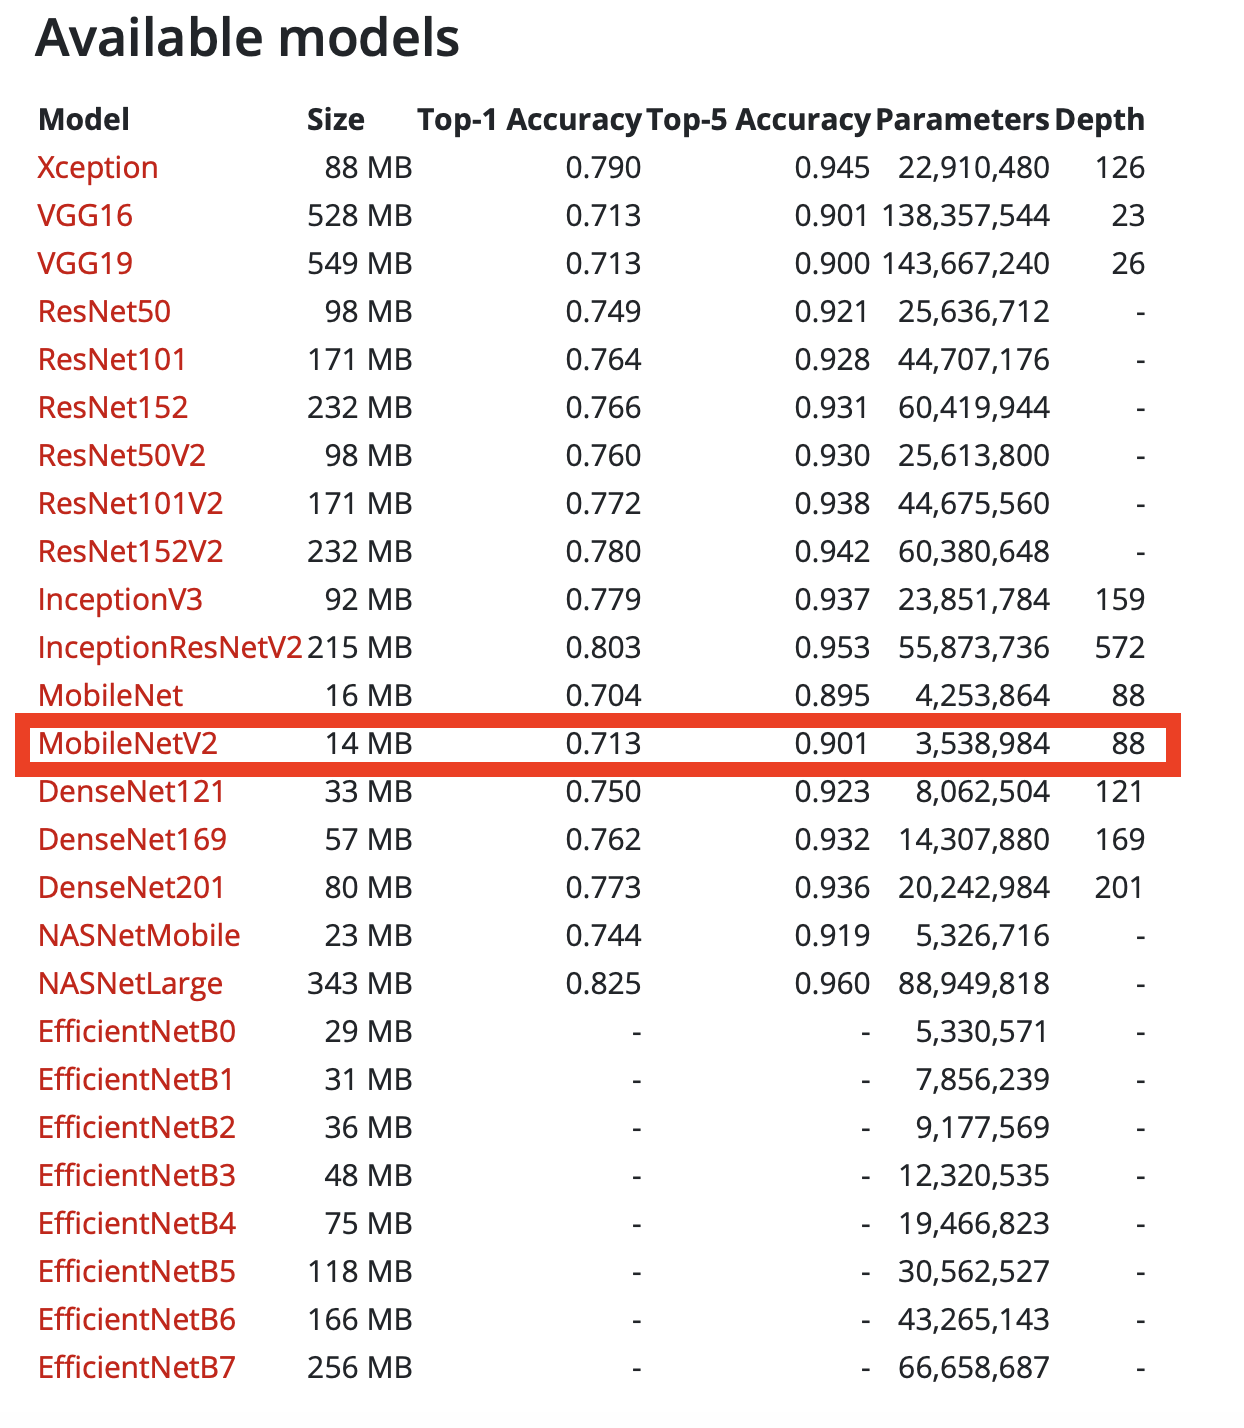
\includegraphics [width=\textwidth*2/3] {mobilenet_vs_rest}
  \caption{MobileNet обладает практически минимальным количеством обучаемых параметров, при этом не отстаёт по точности от других архитектур} 
  \label{img:resnet}  
\end{figure}

           % Глава 2
\chapter{Решение} \label{chapt3}

Данная задача сведена к задаче классификации изображений по N классам. Наличие собаки гарантируется на кадре. Чтобы классифицировать изображение, используется свёрточная нейронная сеть архитектуры ResNet-34 \cite{resnet}.

\begin{figure}[ht] 
  \center
  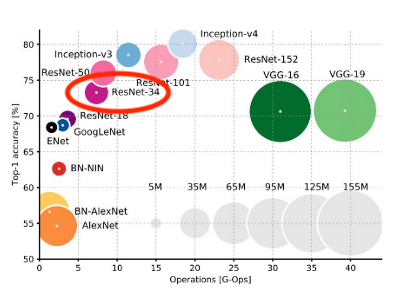
\includegraphics [scale=1] {resnet}
  \caption{Соотношение точности к сложности вычислений у ResNet-34 относительно других архитектур} 
  \label{img:resnet}  
\end{figure}

Для того, чтобы гарантировать исполнение условий, указанных в содержательной постановке задачи, используется предобученная нейронная сеть по сегментации изображений MaskRCNN. Она получает на вход изображение и возвращает маску объектов, находящихся на ней. 

Нас интересуют собаки. Если масок несколько, значит, на кадре больше одной собаки. Если масок собак нет, значит на кадре собак нет. Эти две простые проверки сильно увеличивают качество нейронной сети. 

Помимо этих проверок, маска позволяет убрать ненужную часть кадра, уменьшая шанс того, что нейронная сеть ошибётся.

Также в работе используется MobileNet v2\cite{mobilenet} при работе с маленькими датасетами. Изменения от оригинальной статьи только в так называемой «голове» классификации и размере входного изображения. Структура следующая:

\begin{figure}[ht] 
  \center
  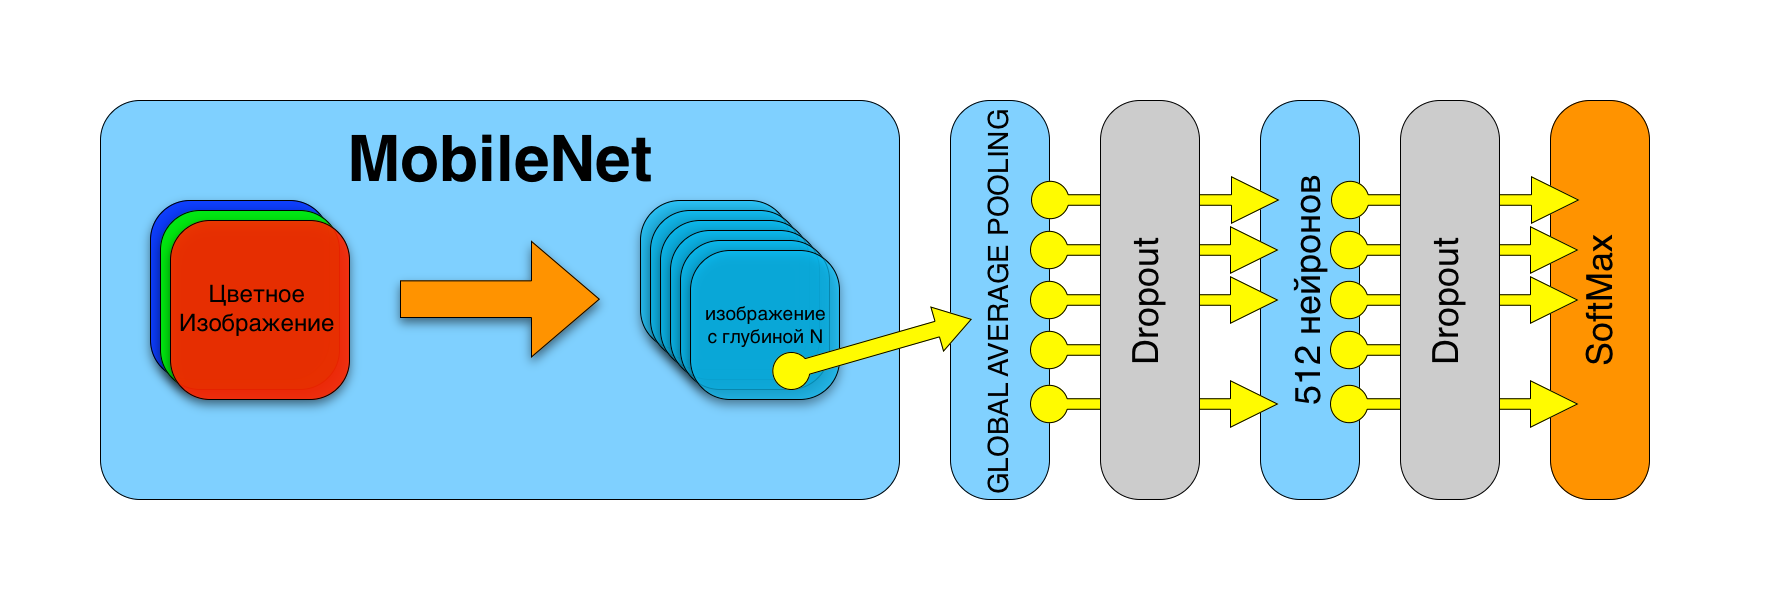
\includegraphics [width=\textwidth] {NN_arch}
  \caption{Архитектура используемой нейронной сети} 
  \label{img:NN_arch}  
\end{figure}

\begin{itemize}
    \item Входное изображение 96х96 пикселей с 3 каналами
    \item Основа MobileNet V2, без "головы"
    \item Global Average Pooling - последняя карта активации(3-мерный тензор) преобразуется в плоский вектор, каждый слой превращается в одно число - среднее по слою. Это позволяет нейронной сети быть инвариантной к размеру входного изображения
    \item Слой DropOut - обнуление 20\% разных значений предыдущего слоя
    \item Batch Norm - нормализация вектора относительно других изображений в мини-партии данных для обучения
    \item Полносвязный слой с 512 нейронами
    \item Функция активации, ReLU
    \item DropOut
    \item BatchNorm
    \item Выходной слой n нейронов, по количеству классов. Функция активации - softmax. 
\end{itemize}

Такая архитектура обусловлена борьбой с переобучением нейронной сети на маленьких объёмах данных. Размер входного изображения держался на минимальном уровне: в то время, как обычно нейронные сети используют по 224 пикселя по длине и 224 ширине, здесь же всего 96. 

Множественные DropOut и Batch Normalization тоже сильно мешают нейронной сети "зазубрить" датасет, так как они каждый раз немного изменяют выходы предыдущих слоёв. Сама архитектура MobileNet тоже выбрана не случайно. Она обладает крайне малым количеством обучаемых параметров, при этом выдаёт совершенно замечательные результаты классификации известных датасетов.\cite{mobilenet}

\begin{figure}[ht] 
  \center
  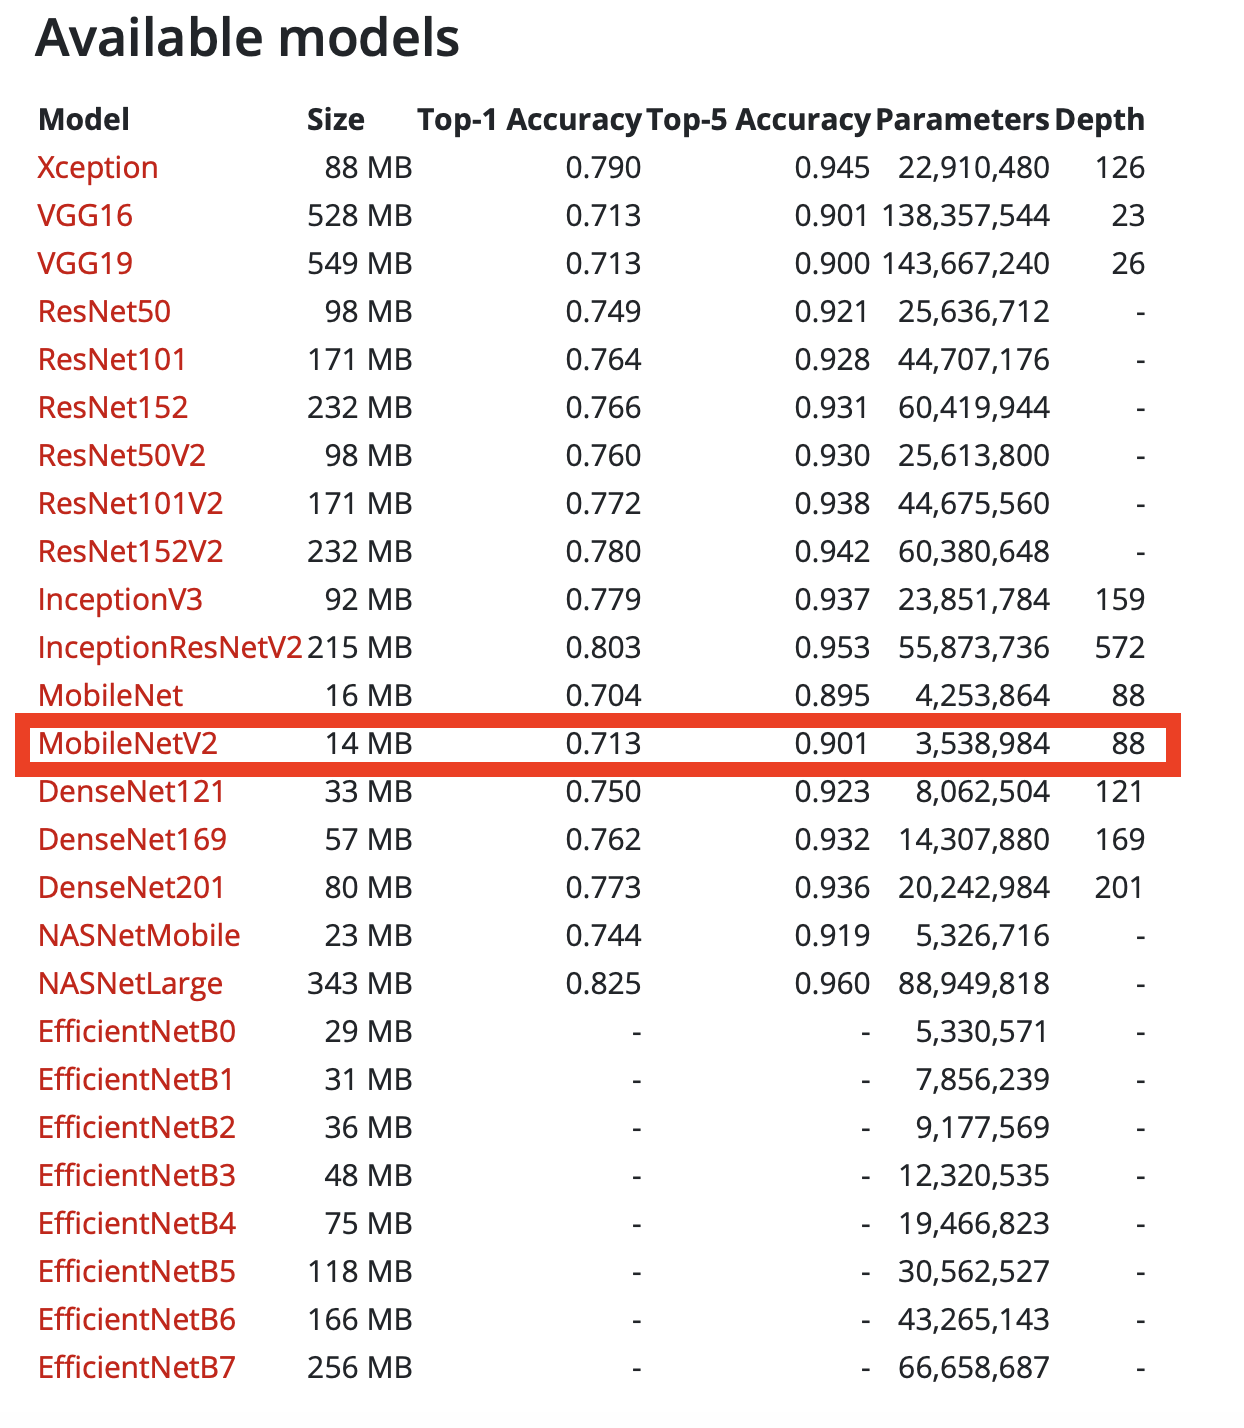
\includegraphics [width=\textwidth*2/3] {mobilenet_vs_rest}
  \caption{MobileNet обладает практически минимальным количеством обучаемых параметров, при этом не отстаёт по точности от других архитектур} 
  \label{img:resnet}  
\end{figure}

\section{Первая итерация} \label{sect3_1}

\subsection{Получение данных}
Для решения задачи классификации нейронной сетью требуется наличие данных для обучения. Датасетов с настоящей задачей в открытом доступе не нашлось, поэтому данные пришлось получать вручную.

\begin{figure}[ht] 
  \center
  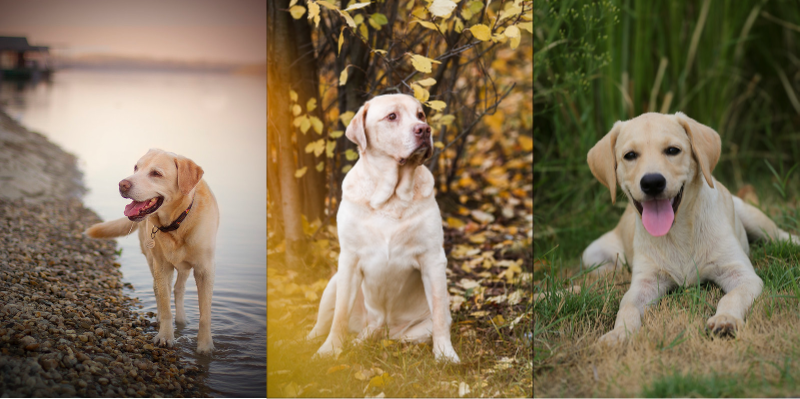
\includegraphics [width=\textwidth*2/3] {dogs-classes}
  \caption{Позы собаки, на которые классифицируются изображения: собака стоит, собака сидит и собака лежит} 
  \label{img:classes}  
\end{figure}

За основу был взят датасет OpenImageDataset\cite{openimages} - набор изображений на более чем тысячу разных классов. Из него был взят подкласс Dog, в котором было 20000 изображений собак. Далее эти данные были размечены на Яндекс.Толоке. 

Каждое изображение было показано пользователю Толоки с вопросом “В какой позиции собака находится на этом фото”. Фотографии были размечены с пятикратным перекрытием, т.е. каждое изображение размечалось пять раз разными людьми. На выходе получился скромного размера датасет, часть изображений в нём не подходили под постановку задач, но на выходе имелась информация о позе собаки, а также об ограничивающей рамке конечностей, с уклоном в будущее.

\subsection{Проверка задачи на решаемость}
Первой целью было поставлено научить нейронную сеть стабильно распознавать позу собаки.

Перед тем, как загружать данные в нейронную сеть, их было решено предобработать. Вместе с комплектом данных из OpenImageDataset шла таблица с информацией о следующем:
\begin{itemize}
    \item Координаты ограничивающей рамки объекта
    \item Список объектов в кадре
    \item Флаг того, что объект загорожен
    \item Флаг того, что объект обрезан
    \item Флаг того, что объект - рисунок объекта, а не фотография
    \item Флаг того, что объект является группой объектов
    \item Флаг того, что объект находится внутри другого объекта
\end{itemize}
В идеальном случае, все флаги должны быть равны нулю - то есть объект не загорожен, не обрезан и не рисунок. Но если применить все фильтры, окажется что из 20000 изображений осталось всего 5000. При этом оказалось так, что флагами может быть отсеяно много годных изображений, но при этом могут остаться и обрезанные и загороженные собаки. В общем, это совсем неконсистентный результат. А вот что действительно могло сильно помочь, так это ограничивающая рамка.

\begin{figure}[ht] 
  \center
  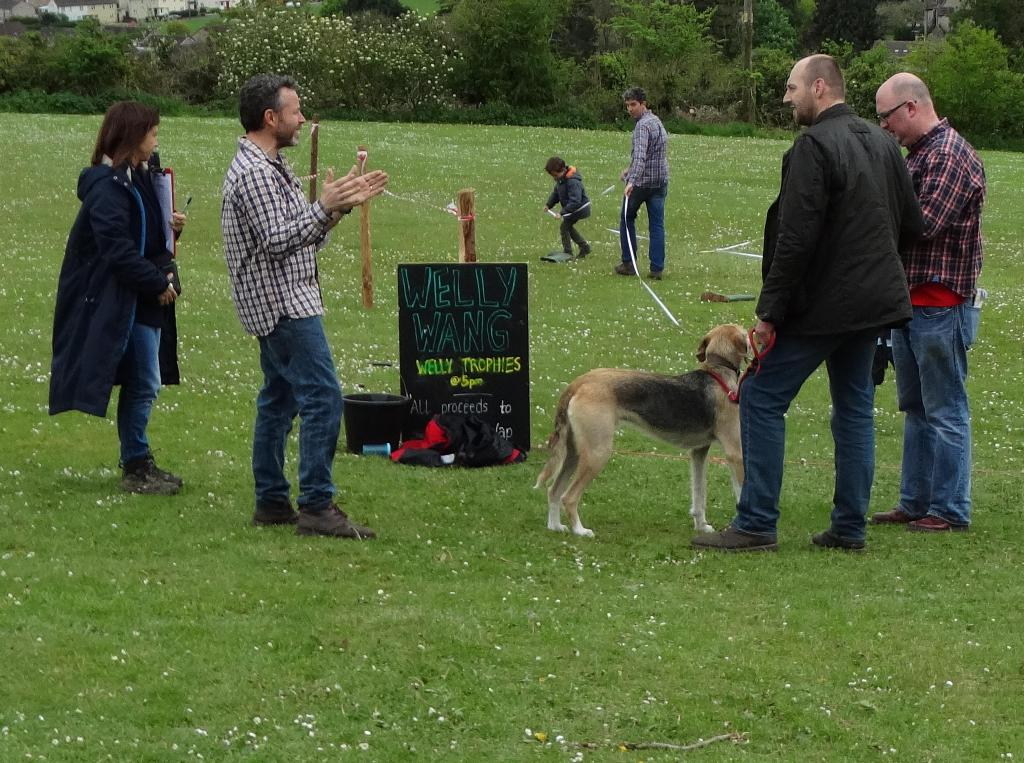
\includegraphics [width=\textwidth*2/3] {crop_helps}
  \caption{Изображение, которому сильно помогло бы обрезание по ограничивающей рамке собаки} 
  \label{img:crop_helps}  
\end{figure}

В теории, свёрточные нейронные сети инвариантны к расположению объектов в кадре, но вот к отвлекающим объектам они не инвариантны. Поэтому на практике обрезание по рамке собаки помогает значительно ускорить процесс обучения нейронной сети и сделать его более стабильным. К тому же, это избавляло бы от множественных собак в кадре.

В итоге были предприняты следующие меры для улучшения работы системы.
\begin{itemize}
    \item Все изображения были обрезаны по ограничивающей рамке собаки. И это дало сильный прирост в качестве классификации, 55\% -> 65\% на 5 классах
    \item Дополнительно были размечены и были удалены из выборки изображения, где собака видна плохо. Это сократило размер и без того маленькой выборки, не сильно улучшив данные, т.к. качество разметки на Толоке достаточно низкое.
    \item Добавлены аугментации обучающей выборки. Аугментации позволяют нейронной сети не запоминать обучающие данные точь-в-точь, что снижает её способность к переобучению.
    \item Проведена очистка изображений. Из обучающей выборки были исключены изображения с несколькими собаками и собаками, которых не видно целиком. Это дало самый ощутимый прирост, но обучающая выборка сократилась до недопустимо маленьких размеров. Добавлено около 3\% точности, 67\%->69\%
    \item Использование transfer learning (переносимость обучения) - все модели, которые использовались здесь, не обучались с нуля. Они обучались на нейронной сети, уже предобученной классифицировать 1000 классов ImageNet(другого открытого датасета с изображениями).
\end{itemize}

Но при всех стараниях, с каким бы фильтром не выбирались данные, как бы изображения не вырезались, какая бы глубина нейронной сети не выбиралась, точность нейронной сети никогда не превышала 67\%. Более того, из-за сильного дизбаланса классов, некоторые категории просто игнорировались классификатором в пользу более популярных. Для сравнения, в категории "собака лежит на спине" насчитывалось всего 400 изображений, против 4500 у категории стоящих собак. 

\subsection{Выводы на основе первой итерации}
Несмотря на трудности в сборе данных и низкое качество классификации нейронной сети, был проведён анализ ошибок и выявлены следующие:
\begin{itemize}
    \item Для разметки данных надо использовать постоянных сотрудников, которым надо уделить время на то, чтобы разобраться с задачей. Низкая цена обучения не компенсирует многократные перекрытия, в надежде найти статистическое среднее.
    \item Количество весов в нейронной сети и количество изображений в датасете должны быть линейно связаны. Хороший размер обучающей выборки для ResNet-34 (2.4 миллиона параметров) - строго от 100 тысяч изображений.
    \item Датасет надо балансировать по количеству изображений в каждом классе.
    \item В данных была огромная внутриклассовая разница между изображениями. У собак множество пород и размеров. Так как точность разметки не идеальна, нейронная сеть может запомнить, что собака сидит, когда она чёрная, например. 
\end{itemize}{}

\section{Вторая итерация}

\subsection{Создание эталонного датасета} \label{subsect3_1_2}
Учитывая прошлые ошибки, было принято решение собрать датасет заново, используя опыт, полученный при разметке первого.

Главные изменения заключаются в следующем:
\begin{enumerate}
    \item Датасет собирается итеративно по небольшим частям и выводы делаются сразу
    \item Размер каждого класса удерживается на одинаковом уровне
    \item Проводится учёт всех изображений, которые тяжело размечать
\end{enumerate}{}

В статье Amy Bearman и Cathering Dong \cite{Bearman2015HumanPE} указывается, что нейронным сетям тяжело распознать позу, при наличии окклюзий, поворотов и переворотов, сильных перспективных искажений, и множественных объектов. В новом датасете было уделено особое внимание трудноклассифицируемым изображениям, поэтому они всячески избегались.

\begin{figure}[ht] 
  \center
  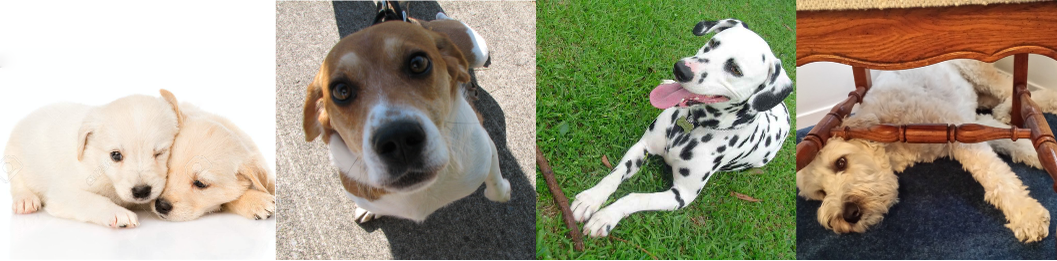
\includegraphics [width=\textwidth] {hazards_dogs}
  \caption{Позы, которые трудно определить: множественные объекты, перспективные искажения, повороты и окклюзии} 
  \label{img:hazards_dogs}  
\end{figure}

На этот раз источником изображений был Flickr. В нём содержится множество фотографий, которые можно было фильтровать
\begin{itemize}
    \item по ориентации - только вертикальные, например.
    \item по породе - можно явно указать, что мы ищем Лабрадора Ретривера
    \item только снятные на телефон
\end{itemize}
В общем, задавать гораздо больше контроля при выборе фотографий.

Собирать фотографии заново было достаточно хорошим упражнением, но главной проблемой были огромные временные затраты на создание датасета даже с 300 фотографиями. Более того, из 80000 фотографий по тегу Лабрадор Ретривер, автором и его ассистентом было просмотрено 70000 из них. И уже из них были собраны 300 фотографий, по 100 изображений на целевой класс. 

\subsection{Попытка решить задачу на мини-наборе данных}
Количество данных накладывает сильные ограничения на выбор архитектуры нейронной сети. Разумеется, с 300 изображениями никаких популярных нынче архитектур не обучить. Но есть одна архитектура, которая смогла справиться с этой задачей. Это ShallowNet - нейронная сеть с одним свёрточным слоем.

\begin{figure}[ht] 
  \center
  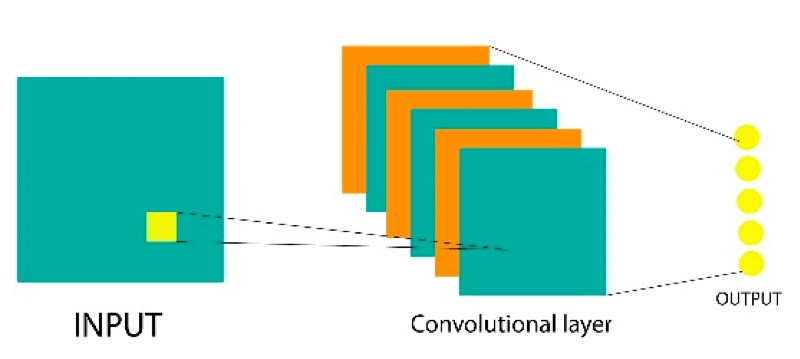
\includegraphics [width=\textwidth*2/3] {ShallowNet-architecture}
  \caption{ShallowNet - Минимально возможная архитектура свёрточной нейронной сети} 
  \label{img:shallownet}  
\end{figure}

Эта архитектура может показаться слишком простой, ведь есть и LeNet, в которой два свёрточных слоя. Но даже назначительное увеличение числа параметров сильно сказывается на переобучении. Все они бесконечно переобучаются, а валидационная точность выходит на плато в районе 50-60\%. Вот, для сравнения, то, с чем приходится иметь дело даже на такой простой архитектуре как LeNet:

\begin{figure}[ht] 
  \center
  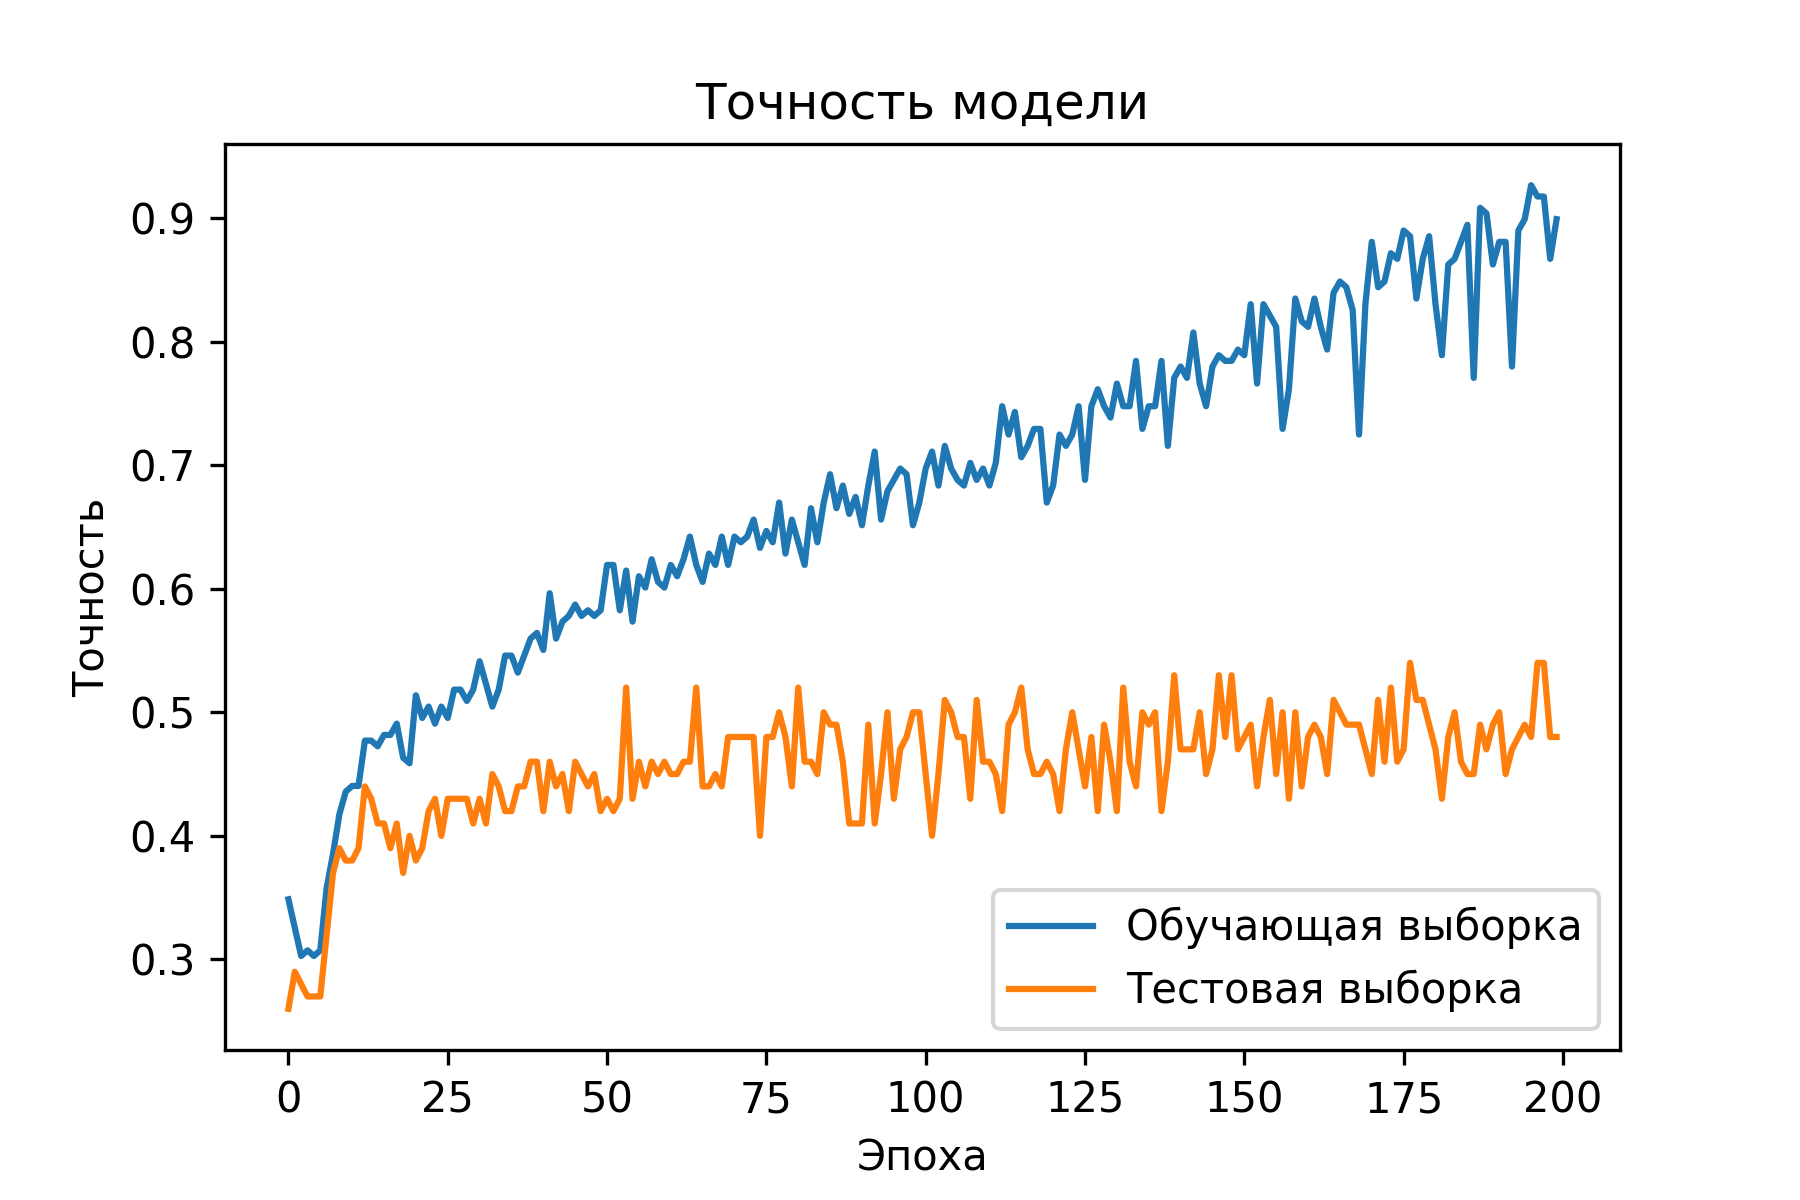
\includegraphics [width=\textwidth*2/3] {accuracy_over_epochs_lenet}
  \caption{Точность нейронной сети на обучающей выборке и на данных, которые нейронная сеть "не видит" при обучении. Можно заметить, тестовая точность выходит на плато ещё на 55 эпохе. Дальше идёт переобучение.} 
  \label{img:shallownet}  
\end{figure}

Таким образом, ShallowNet - это единственная архитектура, на которой валидационная точность, т.е. точность на данных, которые не показывали нейронной сети при обучении, совпадала с теми же при обучении.

Результаты следующие:
\begin{itemize}
    \item При классификации «в лоб» достигается точность в 60\%
    \item При обрезании изображений по ограничительной рамке собаки, точность увеличивается до 68\%
    \item При использовании черно-белых изображений точность также возрастает до 68\%
\end{itemize}

Самым главным выводом создания этого датасета является то, что даже такая маленькая сеть, как ShallowNet научилась распознавать данные с той же точностью, что и большая сеть. Большая сеть не заучивает никаких дополнительных знаний о позе собаки, кроме её геометрической фигуры. 

А стало быть, изображения должны быть хорошо различимы именно как геометрические фигуры. Кроме того, 68\% точности на такой элементарной архитектуре с таким сложным датасетом, это успех. 68\% на трёх классах - это гораздо выше случайного выбора. Случайный выбор дал бы 33\% точность.

\section{Обучение с частичным привлечением учителя} \label{sect3_3}
На основе результатов работы с маленьким, эталонным датасетом, автор попытался повторить успех на более крупном наборе данных с другой архитектурой. В итоге было принято решение просмотреть исходный датасет и повысить точность самих данных. Это достаточно просто, ведь в датасете, к этому моменту уже оставалось всего 5 тысяч фотографий. И, исходя из качества в 70\%, присутствует около 15\% проблемных фотографий, которые достаточно удалить из коллекции, чтобы повысить качество.

После недолгого просмотра фотографий было очевидно, что эти фотографии слишком сильно отличаются от тех, что находятся в эталонном датасете. То есть, человек мог без проблем понять, в какой позе животное изображено.

А вот как геометрические фигуры, собаки не выстраивались в одну картину. И, разумеется, тем самым появляется возможность рационализировать то, что нейронная сеть хорошо распознает. А что - нет, проще спросить у неё самой.

\subsection{Разметка данных нейронной сетью}
Нейронная сеть может сильно помогать в разметке данных. Порой, даже экономя время разметчиков в несколько раз. Главная идея здесь в том, что искать ошибки классификации нейронной сети намного проще, чем размечать данные самому. 
В наличии имелись следующие данные:
\begin{itemize}
    \item датасет с собаками одной породы по 100 изображений на класс
    \item повторно размеченные, "наиболее удачные"
    \footnote{Фотографии, на которых собака одна, и её ничто не загораживает} 
    5000 фотографий из 20000 доступных в OpenImageDataset.
    \item все изображения с классом Dog в OpenImageDataset (их 20000, они не размечены)
\end{itemize}


Также была нейронная сеть, которая с 76\% точностью определяла, сидят собаки, лежат или стоят. Такая точность никуда не годится, если не брать во внимание одну целль. Этого достаточно чтобы узнать у самой нейронной сети какие фотографии ей легко различать, а какие нет.

Проклассифицировав весь датасет, были выбраны только изображения, в которых нейронная сеть не ошиблась, и уверенность была выше 99\%. Таких изображений из 5000 оказалось всего 400, причём 250 из них были те, где собака стоит. И всего 40, где собака сидит. 

Это очень сильный дисбаланс. Но зато все картинки, которые попали в этот крошечный датасет были идеальными. Собралась эталонная поза собак каждой позы.

% и здесь три подборки этих изображений по 20 штук на класс.

\begin{figure}[ht] 
  \center
  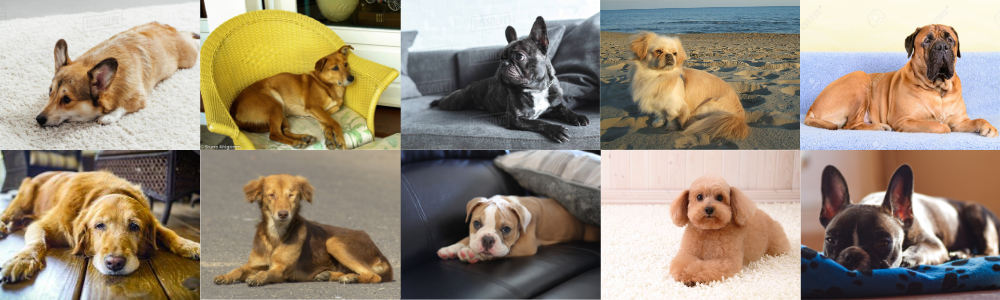
\includegraphics [width=\textwidth] {laying_perfect_dogs}
  \caption{Идеально лежащие собаки} 
  \label{img:laying_perfect_dogs}  
\end{figure}

\begin{figure}[ht] 
  \center
  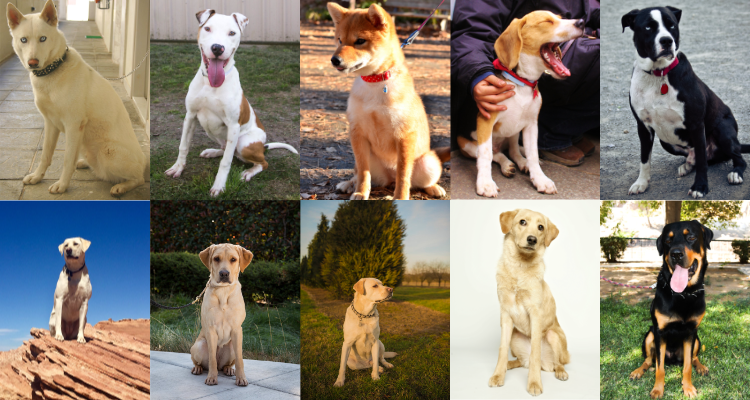
\includegraphics [width=\textwidth] {perfectly_sitting}
  \caption{Идеально сидящие собаки} 
  \label{img:perfectly_sitting}  
\end{figure}

\begin{figure}[ht] 
  \center
  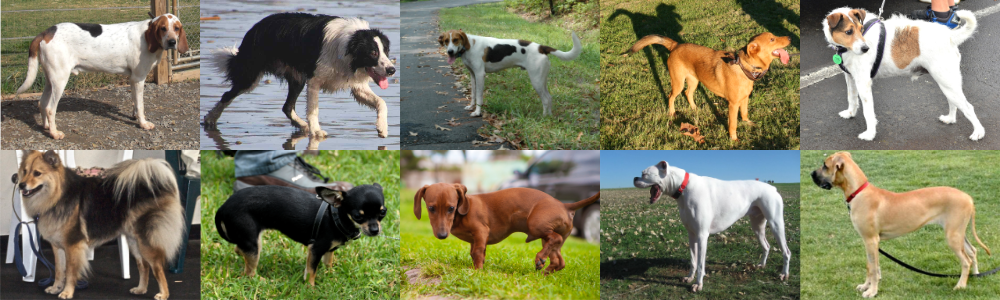
\includegraphics [width=\textwidth] {perfect_standing}
  \caption{Идеально стоящие собаки} 
  \label{img:perfect_standing}  
\end{figure}

Это как раз то, что было нужно. Все собаки были на достаточном отдалении от камеры и все их конечности были хорошо видны, т.е. не загораживали друг друга.

\subsection{Получение датасета}\label{sect3_3_1}

На основе увиденного, было принято решение собрать по этим эталонам больше собак, хотя бы по 500 на класс. В дальнейшем оказалось, что уверенность нейронной сети - относительный параметр. Классы, которые нейронная сеть легко классифицирует, обладают достаточной дисперсией вокруг 100\% вероятности. На практике это означало, что для хорошо подготовленного класса сидячих собак, можно было опустить уверенность сети до 93\%, чтобы иметь схожую вероятность получить эталонные кадры.

Собственно, каждый класс датасета был дополнен лучшими его представителями до одинакового количества изображений на класс. После этого изображения прошли дополнительную чистку на наличие спорных изображений. Это позволило поднять количество изображений до, примерно, 300 на класс.

% спорное изображение, не понятно собака стоит или сидит.
\begin{figure}[ht] 
  \center
  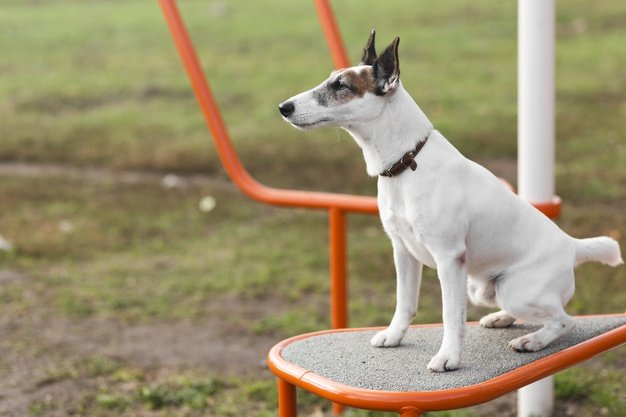
\includegraphics [width=\textwidth*2/3] {sit_or_stand}
  \caption{Спорное изображение, не понятно собака стоит или сидит.} 
  \label{img:laying_perfect_dogs}  
\end{figure}

Окончательно поставить точку в количестве данных позволил всё тот же, плохо размеченный OpenImageDataset. В нём все 20000 изображений были отклассифицированы, и лучшие его представители тоже были отобраны, а затем вручную проверены. В итоге это позволило добавить ещё по 200 изображений на класс до общих 500. 

Получается, выход достаточно небольшой: из 20000 изображений, частью нового датасета стали всего лишь 1500. (Напомним, что предыдущие изображения были тоже взяты из этого датасета).
Недостающие изображения сидячих собак были дополнены 100 фотографиями сидячих лабрадоров из flickr. 

Маленький сет практически идеален, поэтому его можно брать без дополнительной проверки.

\subsection{Результаты на новых данных}\label{sect3_3_2}

Наконец, многообещающий новый датасет можно проверить на практике. Даже когда он ещё не до конца был собран, было ясно что его достаточно просто будет классифицировать.

Для классификации была взята модель MobileNet\cite{mobilenet} с изменённой «головой» классификации. В полносвязные слои быд добавлен DropOut\cite{dropout} с вероятностью 20\% и BatchNorm \cite{batchnorm} - нормализация в пределах текущего фрагмента данных для обучения, с целью не допустить переобучения на столь маленьком наборе данных.

В результате, получилась модель, которая с 96\% валидационной точностью классифицировала этот датасет. Благодаря мерам по регуляризации, точность на отдельной выборке данных была схожа с точностью на обучающих данных.

\begin{figure}[ht] 
  \center
  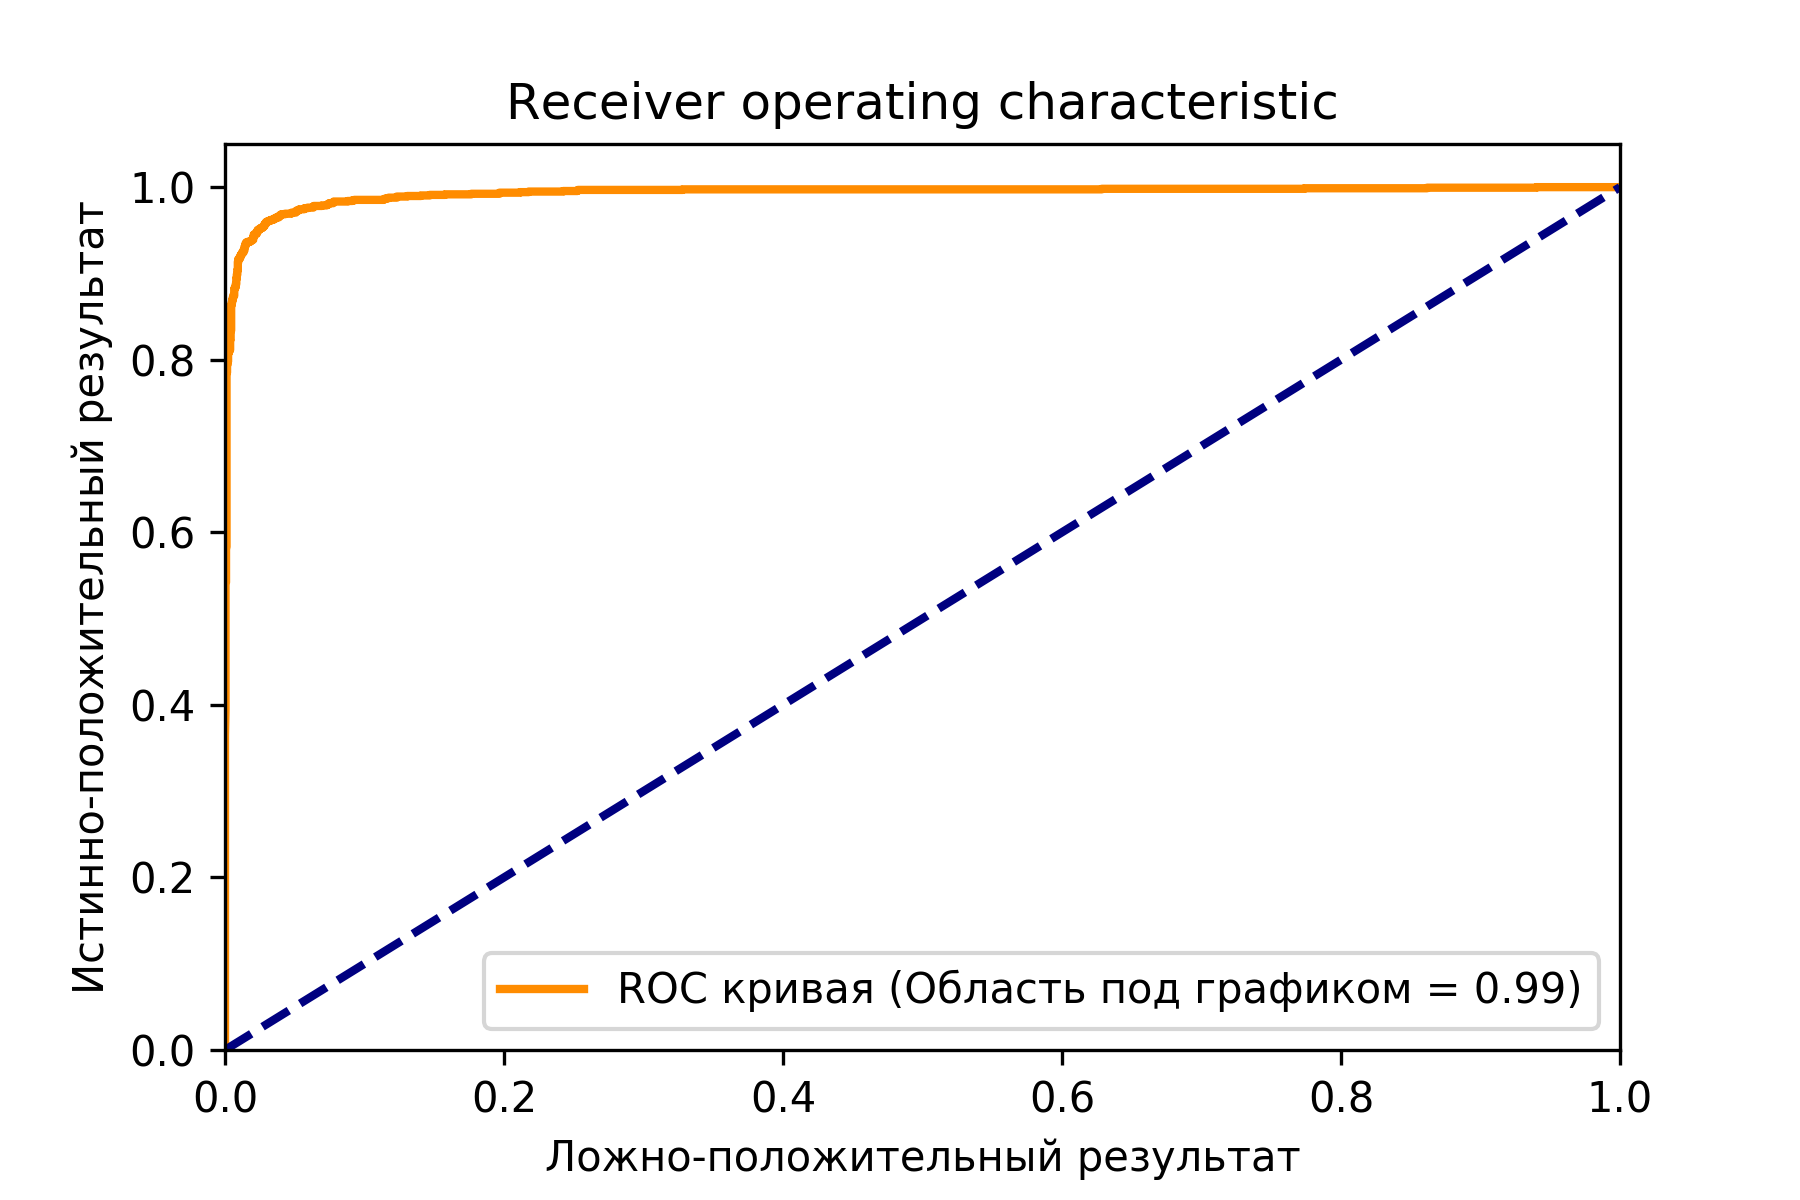
\includegraphics [width=\textwidth*2/3] {ROC_curve}
  \caption{Характеристическая кривая нового классификатора. Чем дальше рыжая кривая лежит от пунктирной линии, тем лучше.} 
  \label{img:ROC_curve}  
\end{figure}

Достоинства:
\begin{itemize}
    \item есть датасет, на котором принципиально возможно обучить нейронную сеть
    \item еочность классификации достаточна для поставленной задачи
    \item создан способ, позволяющий получить датасет любого размера. Требуется только однократная валидация человеком
\end{itemize}


Недостатки:
\begin{itemize}
    \item нейронная сеть в состоянии работать только при удовлетворении множества условий, о которых будет рассказано далее
    \item датасет не предусматривает наличие пограничных случаев, например, когда собака сидит, но не совсем обычным образом - не все позы собаки можно поделить на "сидит", "стоит" и "лежит".
\end{itemize}

Собаки часто лежат на спине, на боку, лежат с поднятой головой ит.д. Собаки ещё бегут, прыгают и кружатся. Все эти случаи не попадают под нашу классификацию.


Итог. Даже при наличии всех недостатков, лучше иметь систему, которая хорошо работает при известных случаях, чем ту, которая совершенно не работает при каждом случае. \cite{karpathy}


\subsection{Расширение датасета}\label{sect3_3_2}
Работать с маленькими датасетами на больших нейронных сетях крайне тяжело. Конечно, предобучение нейронных сетей на крупных наборах данных, таких как ImageNet, сильно помогает обучить глубокие слои и улучшает стабильность обучения, но 1500 изображений, порой, может не хватить даже для обучения «головы» нейронной сети.

Поэтому датасет постепенно расширялся в объёме по схожему принципу, указанному в предыдущей главе. На этот раз источником изображений стала группа «Shiba Inu Photography» в Facebook. В главном альбоме группы содержится 120 тысяч изображений, загруженных владельцами собак породы Шиба Ину.

Из загруженных 20000 изображений, в датасет попало 2205 изображений. То есть, как и изначально, всего 1 изображение из 10 оригинальных попадает в конечный датасет.

Итоговое количество изображений стало уже по 1500 изображений на класс, то есть 4500 изображений. Это уже сравнимо с часто используемыми датасетами как Animal Image Dataset(DOG, CAT and PANDA), в котором содержится по 1000 изображений собак, котов и панд. 


%Второй не такой красивый, но без ограничений (см.~листинг~\ref{list:hwplain}).
%\begin{ListingEnv}[H]
%    \begin{Verb}
%        
%        #include <iostream>
%        using namespace std;
%        
%       int main() //кириллица в комментариях
%        {
%            cout << "Привет, мир" << endl;
%        }
%    \end{Verb}
%    \caption{Программа “Hello, world” без подсветки}
%    \label{list:hwplain}
%\end{ListingEnv}           % Глава 3
\chapter*{Заключение}						% Заголовок
\addcontentsline{toc}{chapter}{Заключение}	% Добавляем его в оглавление

%% Согласно ГОСТ Р 7.0.11-2011:
%% 5.3.3 В заключении диссертации излагают итоги выполненного исследования, рекомендации, перспективы дальнейшей разработки темы.
%% 9.2.3 В заключении автореферата диссертации излагают итоги данного исследования, рекомендации и перспективы дальнейшей разработки темы.
%% Поэтому имеет смысл сделать эту часть общей и загрузить из одного файла в автореферат и в диссертацию:

В результате данной работы была создана система распознавания позы собаки по видеопотоку. Реализацией которого стало мобильное приложение на iOS, которое распознаёт позу собаки по видеопотоку с камеры телефона.

Среди количественных результатов следует отметить что поза собаки, при соблюдении всех условий, классифицируется с точностью 94\%. Скорость работы всей системы на телефоне iPhone 11 составляет 24 кадра в секунду.

Помимо этого, был собран датасет, содержащий 4200 изображений, а также надёжный и быстрый способ расширения этого датасета.

Его можно использовать для распознавания позы собаки, а также, его можно дополнять изображениями других поз и попытаться распознать некоторые сигналы домашних животных.

Что касается распознавания более тяжёлых поз - с этими проблемами возможно бороться. Например, в OpenPose\cite{openpose} успешно борются с окклюзиями конечностей людей и множественными объектами, а значит, при определённой упорности, получится перенести эти технологии в распознавание поз собак.      % Заключение
%\chapter*{Список сокращений и условных обозначений}             % Заголовок
\addcontentsline{toc}{chapter}{Список сокращений и условных обозначений}  % Добавляем его в оглавление

\textbf{КЭН} - Кандидат экономических наук

\textbf{РАН} - Российская академия наук

\textbf{РИТЭГ} - Радиоизотопный термоэлектрический генератор

\textbf{PDF} - Portable Document Format
        % Список сокращений и условных обозначений
%\chapter*{Словарь терминов}             % Заголовок
\addcontentsline{toc}{chapter}{Словарь терминов}  % Добавляем его в оглавление

\textbf{TeX} - Cистема компьютерной вёрстки, разработанная американским профессором информатики Дональдом Кнутом

\textbf{Окклюзия} - когда один объект загораживается другим

\textbf{Машинное обучение} - Семейство компьютерных алгоритмов, которые предполагают вместо прямого решения задачи, обучение на основе известных исходов.


\textbf{Нейронная сеть} - Сложная модель машинного обучения

\textbf{Pose Estimation} - Определение координат тела

\textbf{Датасет} - Набор данных

\textbf{Transfer learning} - Использование обученной нейронной сети для обучения       % Словарь терминов
\clearpage                                  % В том числе гарантирует, что список литературы в оглавлении будет с правильным номером страницы
\phantomsection
\addcontentsline{toc}{chapter}{\bibname}	% Добавляем список литературы в оглавление
%\hypersetup{ urlcolor=black }               % Ссылки делаем чёрными
%\providecommand*{\BibDash}{}                % В стилях ugost2008 отключаем использование тире как разделителя 
\urlstyle{rm}                               % ссылки URL обычным шрифтом
\insertbibliofull                          % Подключаем Bib-базы
\urlstyle{tt}                               % возвращаем установки шрифта ссылок URL
%\hypersetup{ urlcolor={urlcolor} }          % Восстанавливаем цвет ссылок      % Список литературы
%\clearpage
\phantomsection
\addcontentsline{toc}{chapter}{\listfigurename}
\listoffigures									% Список изображений


%%% Список таблиц %%%
% (ГОСТ Р 7.0.11-2011, 5.3.10)
\clearpage
\phantomsection
\addcontentsline{toc}{chapter}{\listtablename}
\listoftables									% Список таблиц
\newpage           % Списки таблиц и изображений (иллюстративный материал)
%\chapter*{Листинг кода обучения нейронной сети} \label{AppendixA}

\begin{python}
import os
import argparse
import numpy as np
import os
import cv2
import matplotlib.pyplot as plt
from sklearn.preprocessing import LabelBinarizer
from sklearn.model_selection import train_test_split
from sklearn.metrics import classification_report, confusion_matrix
from imutils import paths
from skimage.color import rgb2gray
from skimage import exposure
from keras import backend as K
from keras.models import Sequential, Model
from keras.layers.convolutional import Conv2D
from keras.layers.core import Activation, Flatten, Dense
from keras.layers import GlobalAveragePooling2D, Dropout, BatchNormalization
from keras.initializers import glorot_uniform
from keras.optimizers import SGD, Adam
from keras.applications.mobilenet_v2 import MobileNetV2, preprocess_input, decode_predictions
from keras.applications.densenet import DenseNet121
from keras.preprocessing.image import img_to_array
from keras.callbacks import EarlyStopping, ModelCheckpoint

seed = 42

class ImageToArrayPreprocessor:
    def __init__(self, dataFormat=None):
        # store the image data format
        self.dataFormat = dataFormat
        
    def preprocess(self, image):
        # apply the Keras utility function that correctly rearranges # the dimensions of the image
        return img_to_array(image, data_format=self.dataFormat)


class BWPreprocessor:
    def preprocess(self, image):
        return np.expand_dims(rgb2gray(image), 2)


class SimplePreprocessor:
    def __init__(self, width, height, inter=cv2.INTER_AREA):
        # store the target image width, height, and interpolation # method used when resizing
        self.width = width
        self.height = height
        self.inter = inter
        
    def preprocess(self, image):
        # resize the image to a fixed size, ignoring the aspect # ratio
        return cv2.resize(image, (self.width, self.height),
                                interpolation=self.inter)


class PictureControlProcessor:
    def preprocess(self, image):
        image = image.astype("float") / 255.0
        img_adapteq = exposure.equalize_hist(image)
        return img_adapteq


class SimpleDatasetLoader:
    
    def __init__(self, preprocessors=None):
        # store the image preprocessor
        self.preprocessors = preprocessors

        # if the preprocessors are None, initialize them as an
        # empty list
        if self.preprocessors is None:
            self.preprocessors = []
            
    def load(self, imagePaths, verbose=-1):
        # initialize the list of features and labels
        data = []
        labels = []

        # loop over the input images
        for (i, imagePath) in enumerate(imagePaths):
            # load the image and extract the class label assuming
            # that our path has the following format:
            # /path/to/dataset/{class}/{image}.jpg
            image = cv2.imread(imagePath)
            label = imagePath.split(os.path.sep)[-2]
            if self.preprocessors is not None:
                for p in self.preprocessors:
                    image = p.preprocess(image)
            
            # treat our processed image as a "feature vector" # by updating the data list followed by the labels 
            data.append(image)
            labels.append(label)
            # show an update every ‘verbose‘ images
            if verbose > 0 and i > 0 and (i + 1) % verbose == 0: 
                print("[INFO] processed {}/{}".format(i + 1, len(imagePaths)))
            # return a tuple of the data and labels
        return (np.array(data), np.array(labels))


class ShallowNet:
    @staticmethod
    def build(width, height, depth, classes):
        # initialize the model along with the input shape to be
        # "channels last"
        model = Sequential()
        inputShape = (height, width, depth)
        # if we are using "channels first", update the input shape
        if K.image_data_format() == "channels_first":
            inputShape = (depth, height, width)
        
        # define the first (and only) CONV => RELU layer
        model.add(Conv2D(32, (3, 3), padding="same", input_shape=inputShape))
        model.add(Activation("relu"))
        # softmax classifier
        model.add(Flatten())
        model.add(Dense(classes))
        model.add(Activation("softmax"))

        # return the constructed network architecture
        return model

class MyMobileNet:
    @staticmethod
    def build(width, height, depth, classes, trainable_conv=False):
        base_model = MobileNetV2(include_top=False, input_shape=(width, height, 3))
        for layer in base_model.layers:
            layer.trainable=trainable_conv
        x = base_model.output
        x = GlobalAveragePooling2D()(x)
        x = Dropout(rate = .2)(x)
        x = BatchNormalization()(x)
        x = Dense(512, activation='relu')(x)
        x = Dropout(rate = .2)(x)
        x = BatchNormalization()(x)
        predictions = Dense(classes, activation='softmax')(x)
        model = Model(inputs=base_model.input, outputs=predictions)
        return model

def balance_classes(data, labels):
    class_names, counts = np.unique(labels, return_counts=True)
    amount = counts.min()
    new_data = []
    new_labels = []
    for c in class_names:
        new_data.append(data[labels == c][:amount])
        new_labels.append(labels[labels == c][:amount])
    new_labels = np.array(new_labels).reshape(-1)
    new_data = np.vstack(np.array(new_data))
    return new_data, new_labels

def step_decay(epoch):
    initial_lrate = 0.1
    drop = 0.5
    epochs_drop = 10.0
    lrate = initial_lrate * math.pow(drop, math.floor((1+epoch)/epochs_drop))
    return lrate

#PARAMETERS
args = {'dataset':'data/best_combined'}
imagePaths = list(paths.list_images(args["dataset"]))
model_class = 'MobileNet'
imsize = 96


sp = SimplePreprocessor(imsize, imsize)
iap = ImageToArrayPreprocessor()
bw = BWPreprocessor()
pc = PictureControlProcessor()

preprocessors = [sp, iap]
sdl = SimpleDatasetLoader(preprocessors=preprocessors)
(data, labels) = sdl.load(imagePaths, verbose=500)
data = data.astype("float") / 255.0

data, labels = balance_classes(data, labels)

(trainX, testX, trainY, testY) = train_test_split(data, labels, test_size=200, random_state=seed)

lb = LabelBinarizer().fit(labels)
trainY = lb.transform(trainY)
testY = lb.transform(testY)
class_names = np.unique(labels)

lrate = LearningRateScheduler(step_decay)
chkpt = ModelCheckpoint(filepath='best_model.h5', monitor='val_loss', save_best_only=True)
early_stop = EarlyStopping(monitor='val_loss', patience=20)
callbacks = [lrate,
            chkpt,
            early_stop]
            
print("[INFO] compiling model...", end='\r')
if model_class == "ShallowNet":
    epochs = 200
    opt = Adam(lr=0.03, decay=1e-3/epochs)
    model = ShallowNet.build(width=imsize, height=imsize, depth=trainX[0].shape[2], classes=3)
elif model_class == "LeNet":
    epochs = 200
    opt = Adam(lr=0.03, decay=1e-3/epochs)
    model = LeNet.build(width=imsize, height=imsize, depth=trainX[0].shape[2], classes=3)
elif model_class == "MobileNet":
    epochs = 100
    opt = Adam(lr=0.03)
    model = MyMobileNet.build(width=imsize, height=imsize, depth=trainX[0].shape[2], classes=trainY[0].shape[0])

print("[INFO] compiling model... Done")

print("[INFO] training network...")
np.random.seed(seed)
H = model.fit(trainX, trainY, 
              validation_data=(testX, testY), 
              batch_size=32, 
              epochs=50, 
              verbose=1,
              callbacks=callbacks
             )
print("[INFO] model finished training")

history = H
print(history.history.keys())
# summarize history for accuracy
plt.plot(history.history['acc'])
plt.plot(history.history['val_acc'])
plt.title('model accuracy')
plt.ylabel('accuracy')
plt.xlabel('epoch')
plt.legend(['train', 'test'], loc='upper left')
plt.show()
# summarize history for loss
plt.plot(history.history['loss'])
plt.plot(history.history['val_loss'])
plt.title('model loss')
plt.ylabel('loss')
plt.xlabel('epoch')
plt.legend(['train', 'test'], loc='upper left')
plt.show()

model.load_weights('best_model.h5')

predictions = model.predict(testX, batch_size=32) 
print(classification_report(testY.argmax(axis=1),
    predictions.argmax(axis=1), target_names=class_names))


print(confusion_matrix(testY.argmax(axis=1),
    predictions.argmax(axis=1), normalize='true'))

print("[INFO] Complete! Weights are located in file best_model.h5")

\end{python}
%\lstinputlisting[language={Python},caption={Исходный код модуля для обучения нейронной сети},label={list:external1}]{listings/train.py}
        % Приложения

\end{document}
